% !TeX root = ../analysisnote.tex

\section{Appendix}

\section{PID cuts and acceptance plots}

\begin{table}
    \centering
    \begin{tabular}{|c|c|c|c|c|c|} \hline 
         &  $\pi^+$&  $\pi^-$&  $K^+$&  $K^-$& p\\ \hline 
         3.0 GeV&  \makecell{$|n\sigma_{\pi}|<3$,\\$-0.1<m^2<0.15$} &  \makecell{$|n\sigma_{\pi}|<3$,\\$-0.1<m^2<0.15$} & \makecell{$|n\sigma_{K}|<3$,\\ $0.16<m^2<0.36$} &  \makecell{$|n\sigma_{K}|<3$,\\ $0.16<m^2<0.36$} & \makecell{$p<2GeV/c$,\\$|n\sigma_p-shift|<2$; \\$p>2GeV/c$,\\$|n\sigma_p-shift| < 2$, \\$0.6<m^2<1.2$}\\ \hline 
         3.2 GeV&  \makecell{$0.2<p<0.7GeV/c$,\\$|n\sigma_\pi-shift|<3$; \\$0.7<p<3.0GeV/c$,\\$|n\sigma_\pi-shift| < 3$, \\$-0.1<m^2<0.15$}&  \makecell{$0.2<p<3.7GeV/c$,\\$|n\sigma_\pi-shift|<3$}&  \makecell{$0.2<p<2.1GeV/c$,\\$|n\sigma_K-shift|<3$, \\$0.16<m^2<0.36$; \\$2.1<p<2.6GeV/c$,\\$|n\sigma_K-shift| < 3$, \\$0.2<m^2<0.33$}&  \makecell{$0.2<p<1.3GeV/c$,\\$|n\sigma_K-shift|<3$, \\$0.16<m^2<0.36$; \\$1.3<p<2.1GeV/c$,\\$|n\sigma_K-shift| < 3$, \\$0.19<m^2<0.36$}& \makecell{$0.2<p<1.3GeV/c$,\\$|n\sigma_p-shift|<3$; \\$1.3<p<4.5GeV/c$,\\$|n\sigma_p-shift| < 3$, \\$0.6<m^2<1.2$}\\ \hline 
         3.5 GeV&  \makecell{$0.2<p<0.7GeV/c$,\\$|n\sigma_\pi-shift|<3$; \\$0.7<p<3.0GeV/c$,\\$|n\sigma_\pi-shift| < 3$, \\$-0.1<m^2<0.15$}&  \makecell{$0.2<p<3.7GeV/c$,\\$|n\sigma_\pi-shift|<3$}&  \makecell{$0.2<p<2.3GeV/c$,\\$|n\sigma_K-shift|<3$, \\$0.16<m^2<0.36$; \\$2.3<p<2.7GeV/c$,\\$|n\sigma_K-shift| < 3$, \\$0.2<m^2<0.33$}&  \makecell{$0.2<p<1.6GeV/c$,\\$|n\sigma_K-shift|<3$, \\$0.16<m^2<0.36$; \\$1.6<p<2.4GeV/c$,\\$|n\sigma_K-shift| < 3$, \\$0.19<m^2<0.36$}& \makecell{$0.2<p<1.2GeV/c$,\\$|n\sigma_p-shift|<3$; \\$1.2<p<4.5GeV/c$,\\$|n\sigma_p-shift| < 3$, \\$0.6<m^2<1.2$}\\ \hline 
         3.9 GeV&  \makecell{$0.2<p<0.7GeV/c$,\\$|n\sigma_\pi-shift|<3$; \\$0.7<p<3.0GeV/c$,\\$|n\sigma_\pi-shift| < 3$, \\$-0.1<m^2<0.15$}&  \makecell{$0.2<p<3.7GeV/c$,\\$|n\sigma_\pi-shift|<3$}&  \makecell{$0.2<p<2.1GeV/c$,\\$|n\sigma_K-shift|<3$, \\$0.16<m^2<0.36$; \\$2.1<p<2.6GeV/c$,\\$|n\sigma_K-shift| < 3$, \\$0.2<m^2<0.33$}&  \makecell{$0.2<p<1.3GeV/c$,\\$|n\sigma_K-shift|<3$, \\$0.16<m^2<0.36$; \\$1.3<p<2.1GeV/c$,\\$|n\sigma_K-shift| < 3$, \\$0.19<m^2<0.36$}& \makecell{$0.2<p<1.2GeV/c$,\\$|n\sigma_p-shift|<3$; \\$1.2<p<4.5GeV/c$,\\$|n\sigma_p-shift| < 3$, \\$0.6<m^2<1.2$}\\ \hline
    \end{tabular}
    \caption{PID cut for $\pi, K, p$ at 3.0, 3.2, 3.5, 3.9 GeV}
    \label{tab:pid_piKp}
\end{table}


\begin{figure}[hbt!]
\centering
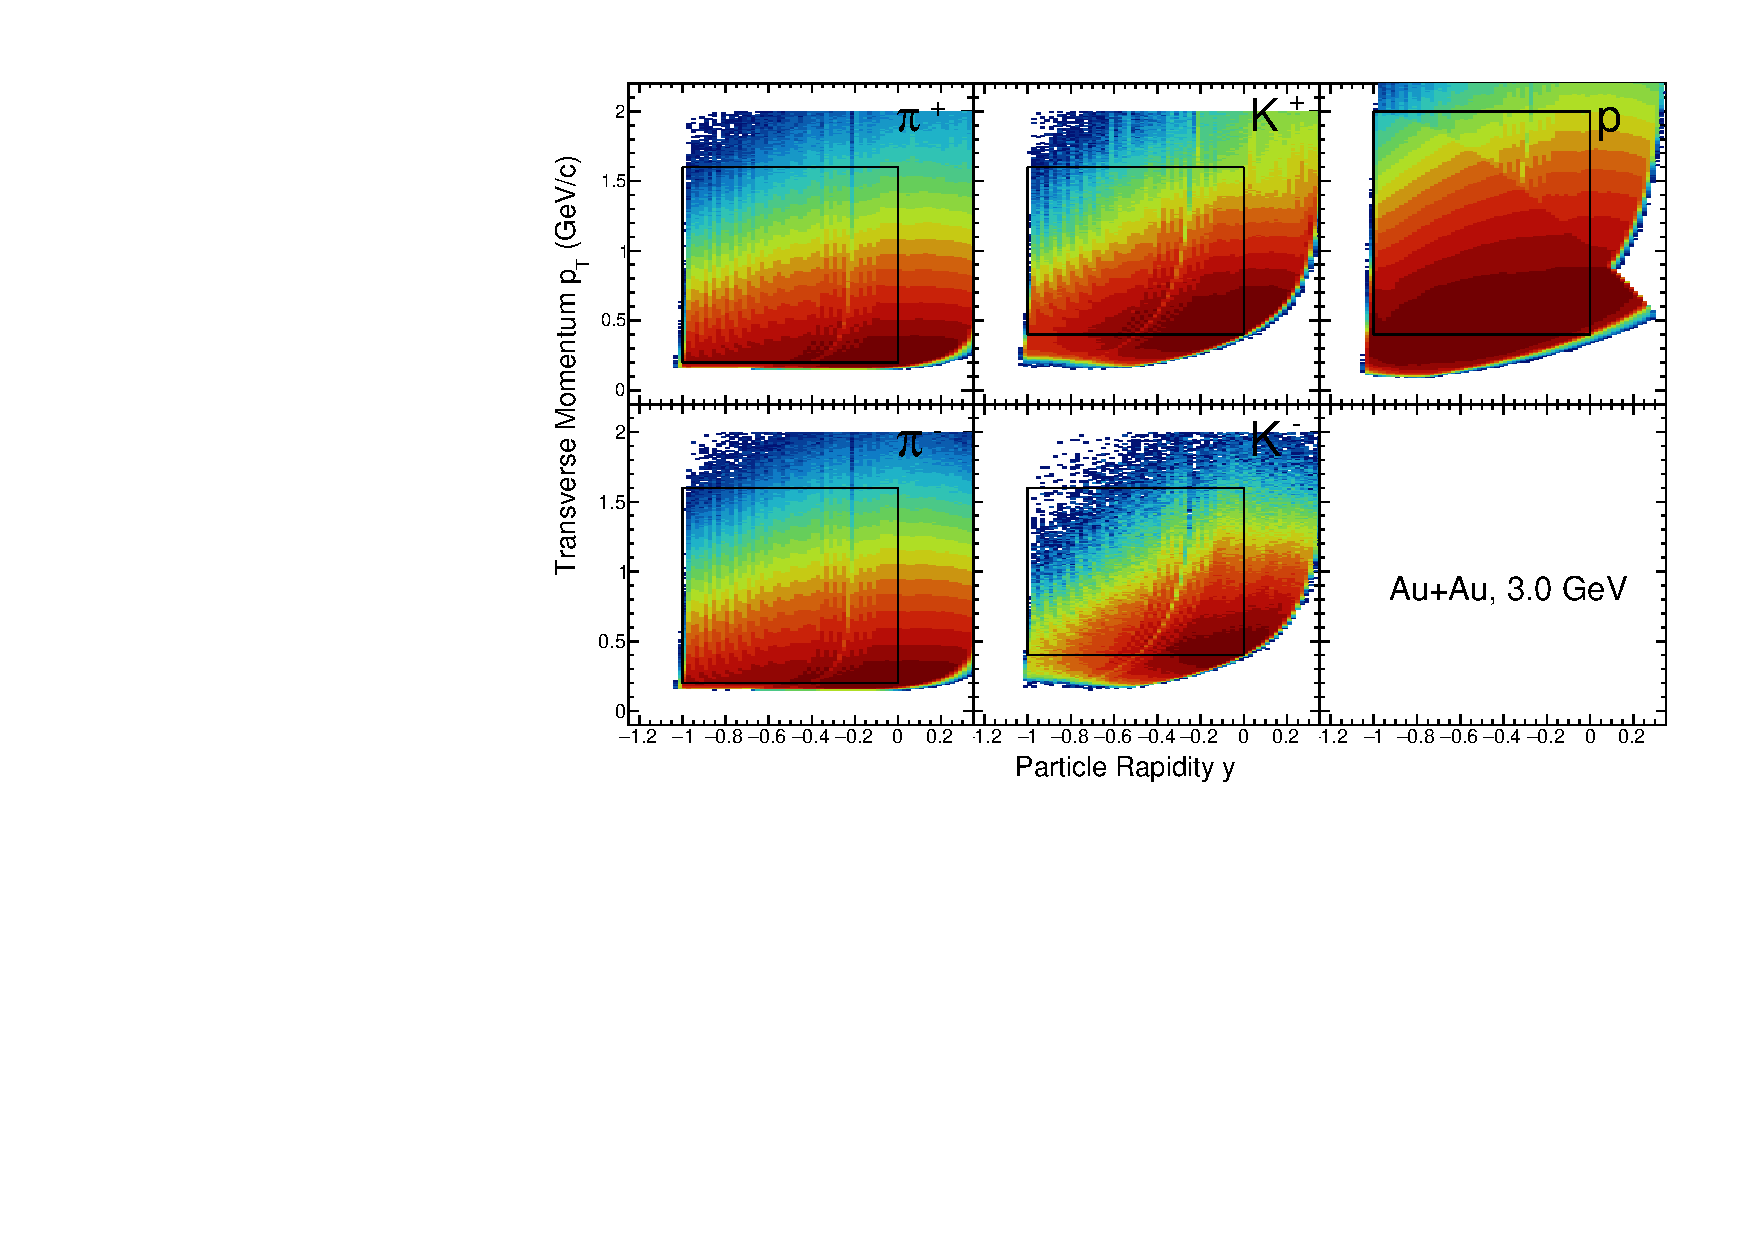
\includegraphics[width=0.55\linewidth]{figures/chapter02/3gev_piKp_acceptance.pdf}
\caption{$\pi, K, p$ density distribution as function of rapidity and transverse momentum at $\sqrt{s_{NN}}$ = 3.0 GeV.}
\label{fig:3gev_piKp_acceptance}
\end{figure}


\begin{figure}[hbt!]
\centering
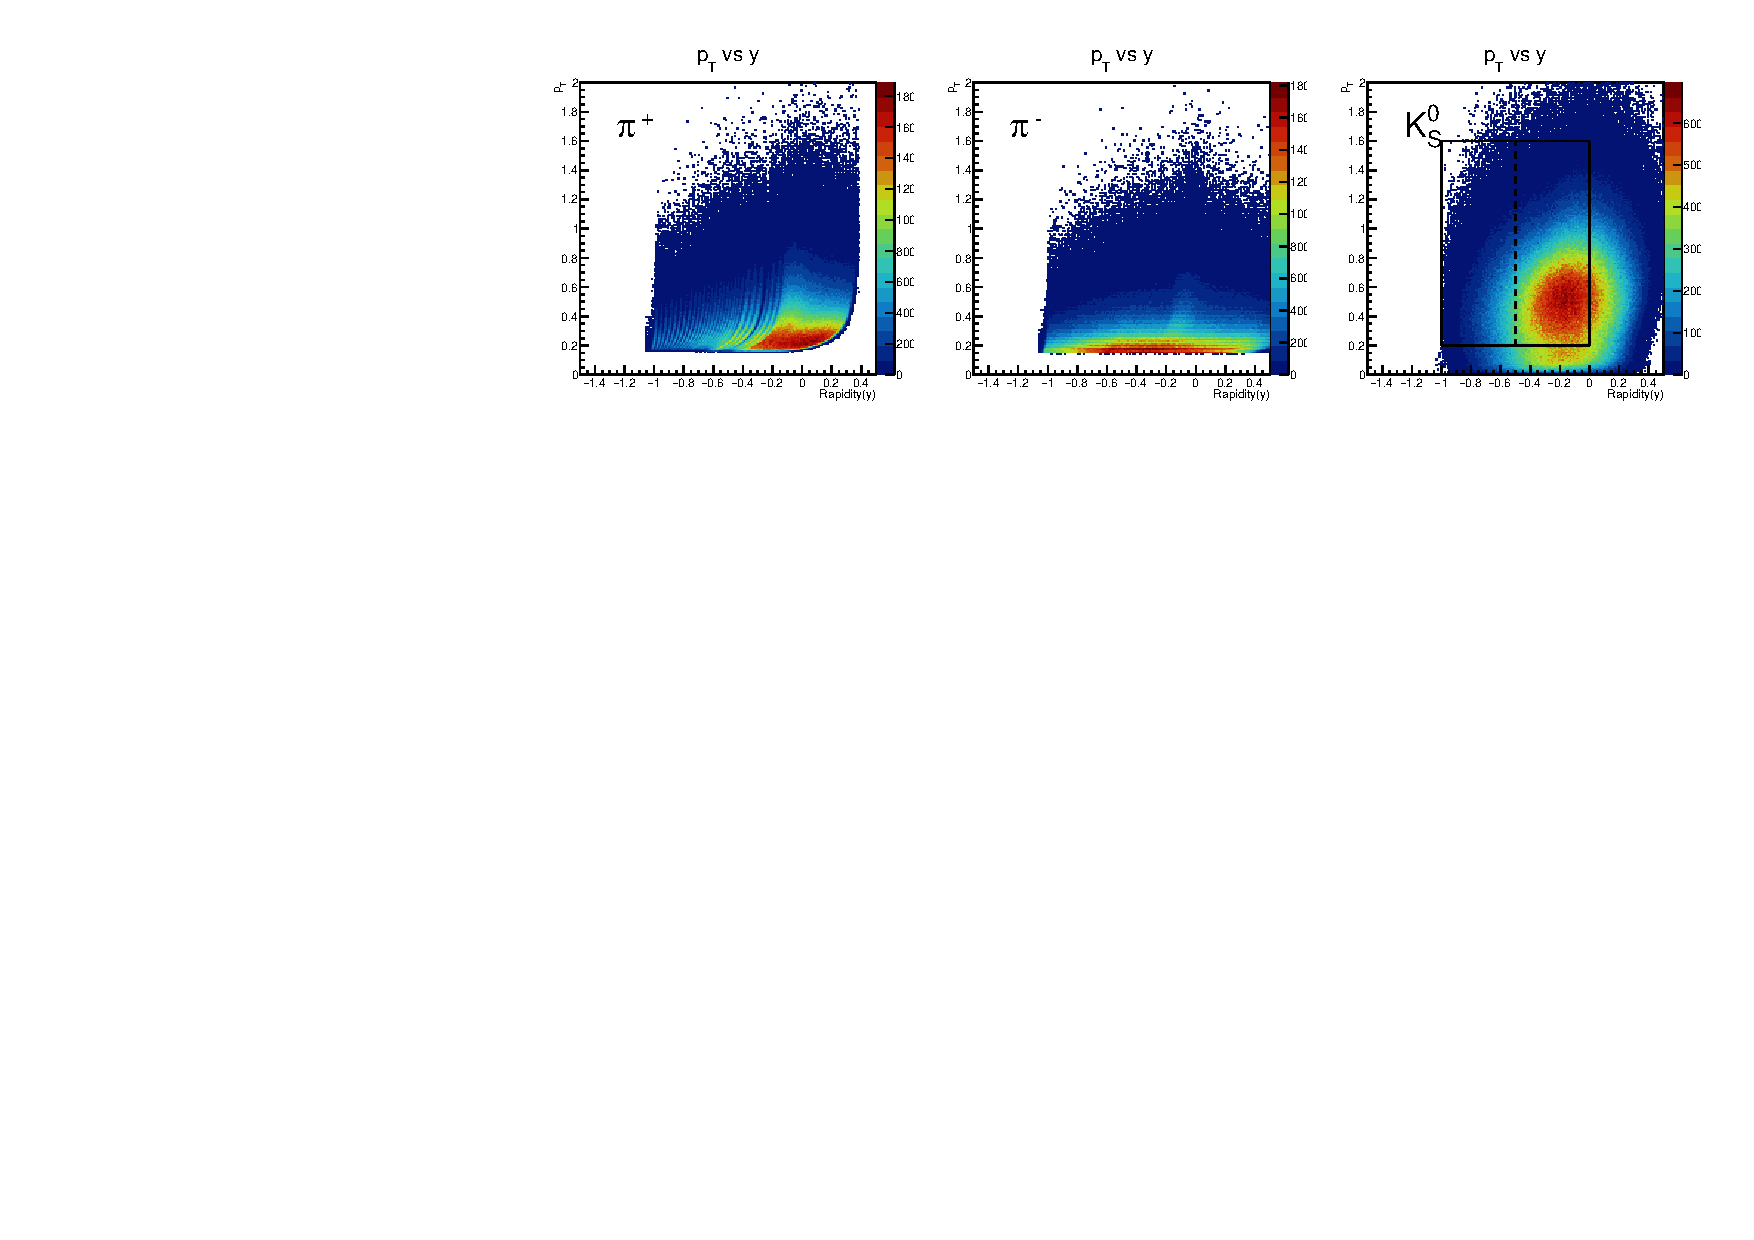
\includegraphics[width=0.55\linewidth]{figures/chapter02/3gev_K0s_acceptance.pdf}
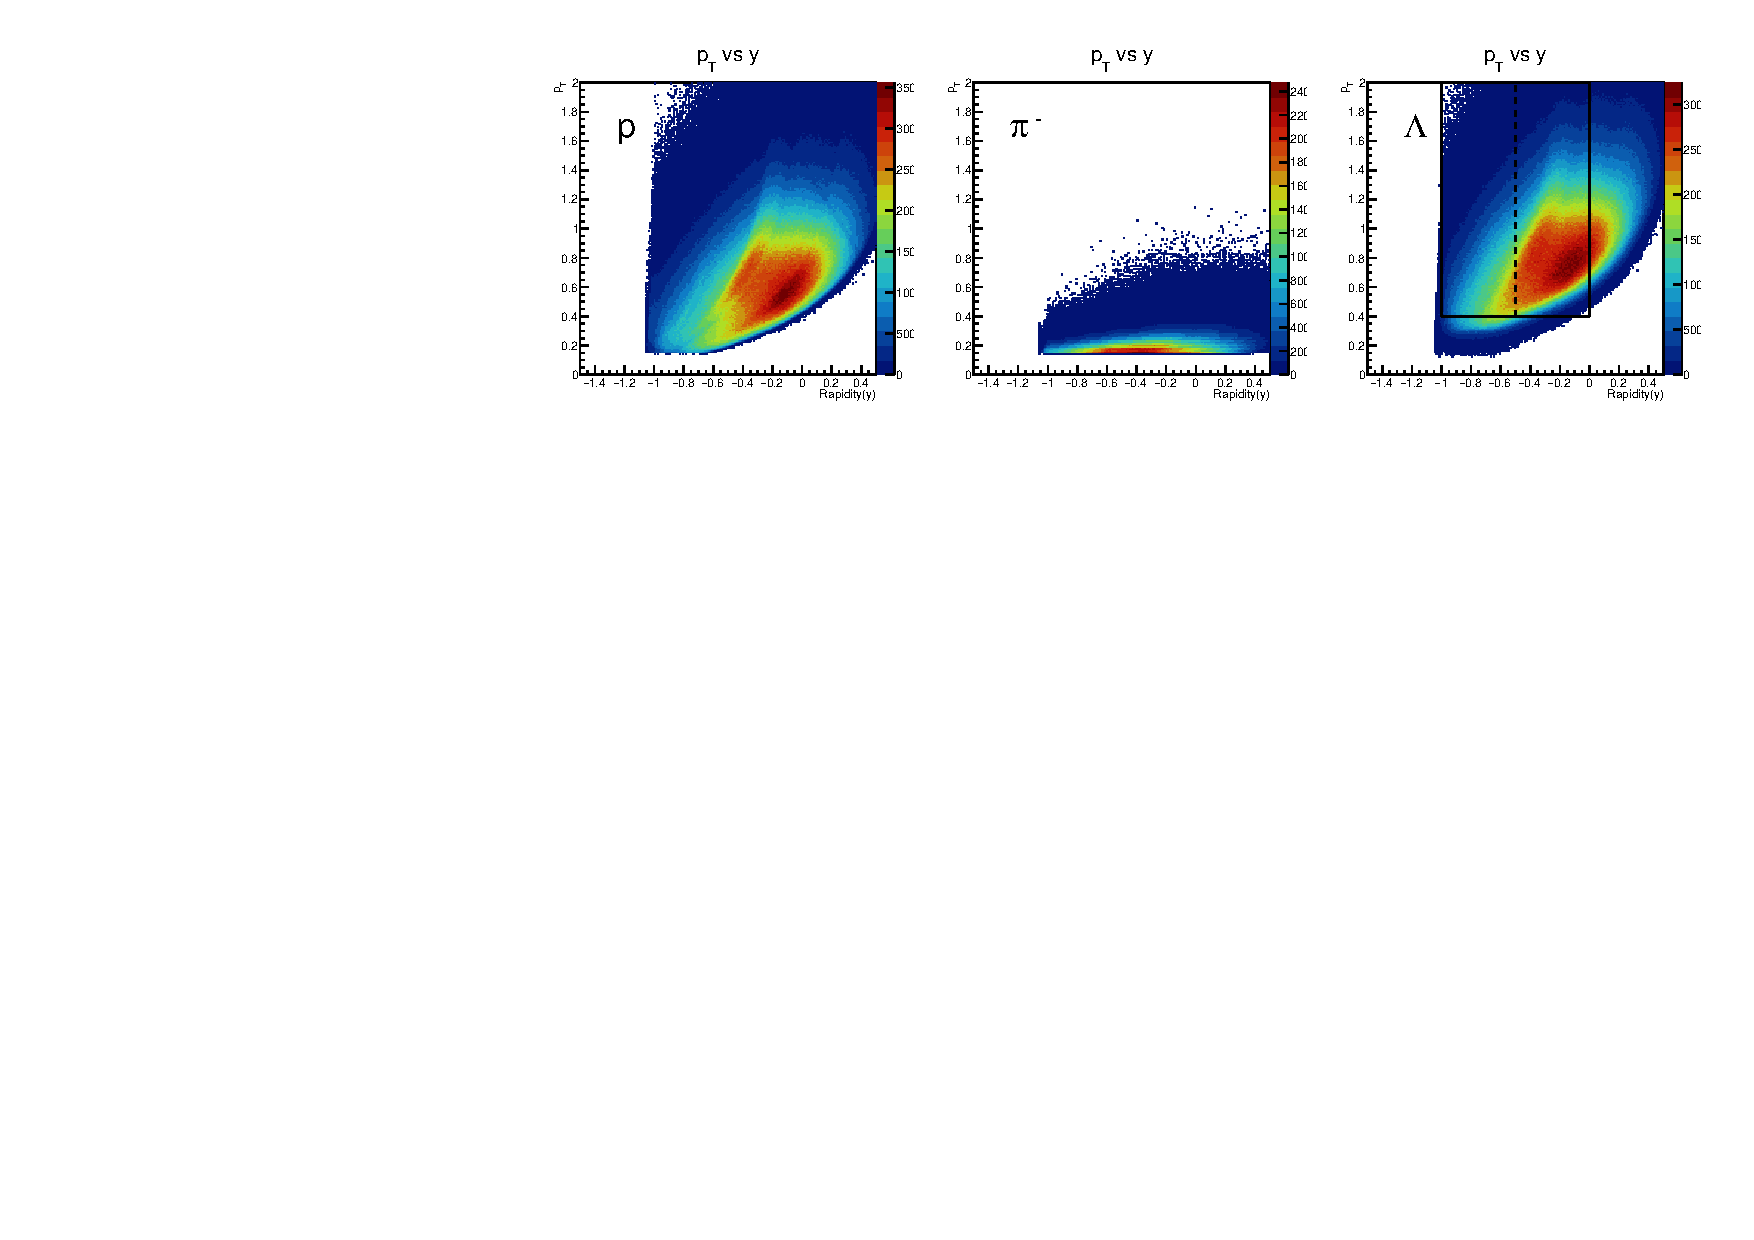
\includegraphics[width=0.55\linewidth]{figures/chapter02/3gev_lambda_acceptance.pdf}
\caption{$K^{0}_{S}~and~\Lambda$(and their daughters) density distribution as function of rapidity and transverse momentum at $\sqrt{s_{NN}}$ = 3.0 GeV.}
\label{fig:3gev_K0s_lambda_acceptance}
\end{figure}


\begin{figure}[hbt!]
\centering
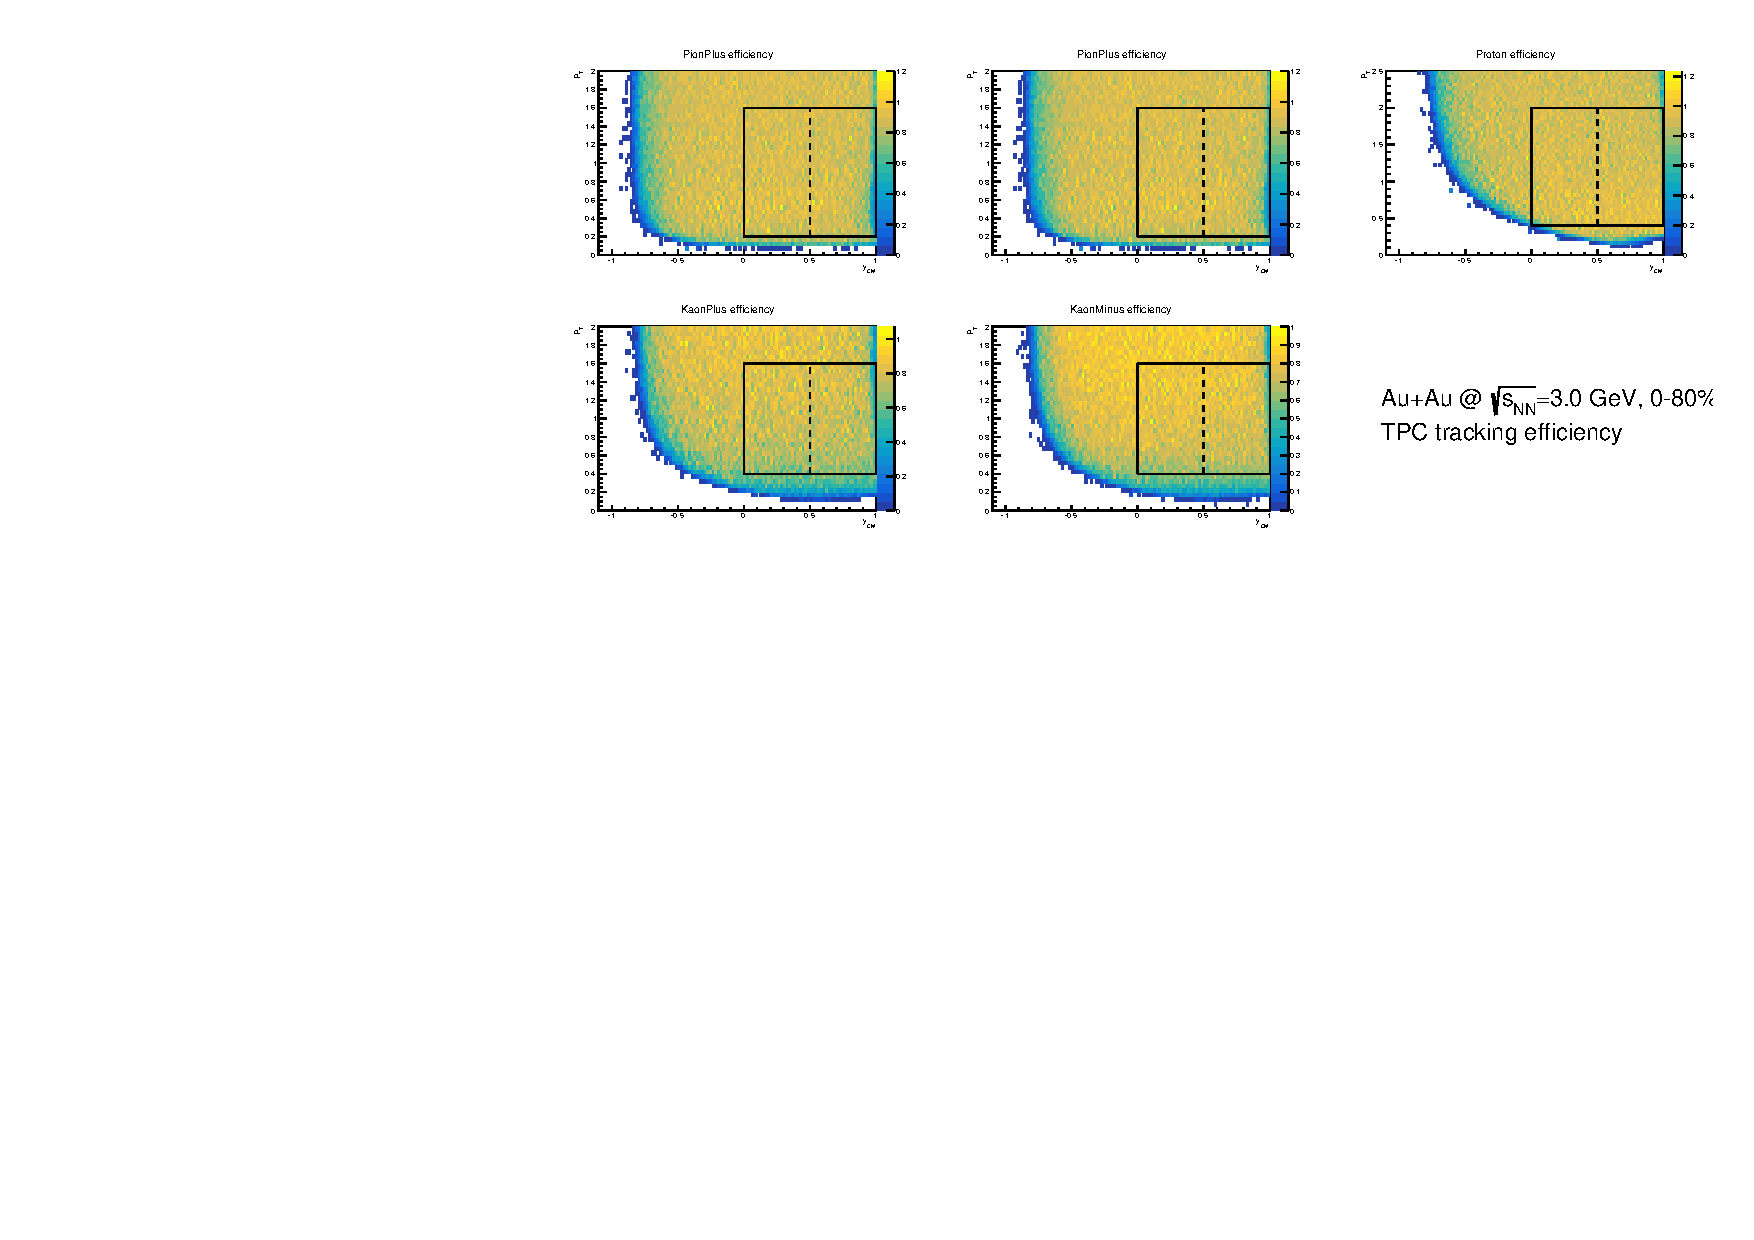
\includegraphics[width=0.65\linewidth]{figures/chapter02/3gev_TPC_eff.pdf}
\caption{TPC tracking efficiency of $\pi, K, p$ as function of rapidity y and transverse momentum $p_T$ at $\sqrt{s_{NN}}$ = 3.0 GeV.}
\label{fig:3gev_piKp_TPCeff}
\end{figure}

\begin{figure}[hbt!]
\centering
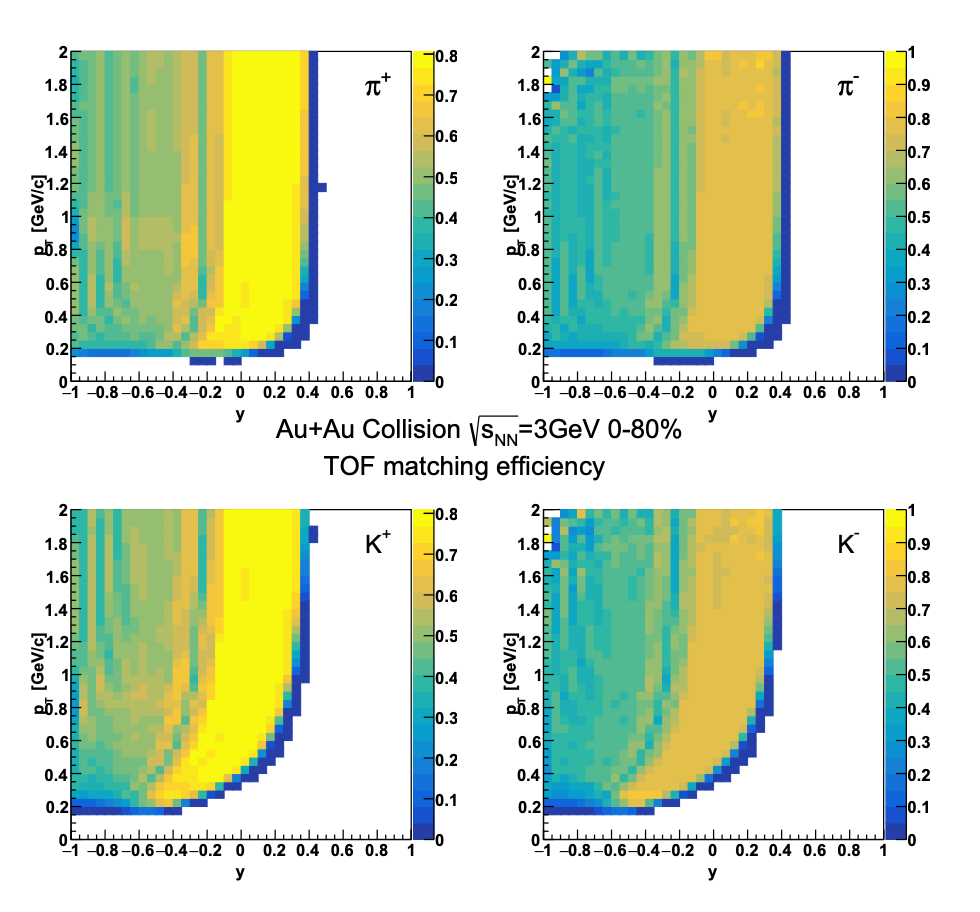
\includegraphics[width=0.55\linewidth]{figures/chapter02/3gev_TOF_eff.png}
\caption{TOF matching efficiency of $\pi, K$ as function of rapidity y and transverse momentum $p_T$ at $\sqrt{s_{NN}}$ = 3.0 GeV.}
\label{fig:3gev_piKp_TOFeff}
\end{figure}

\begin{figure}[hbt!]
\centering
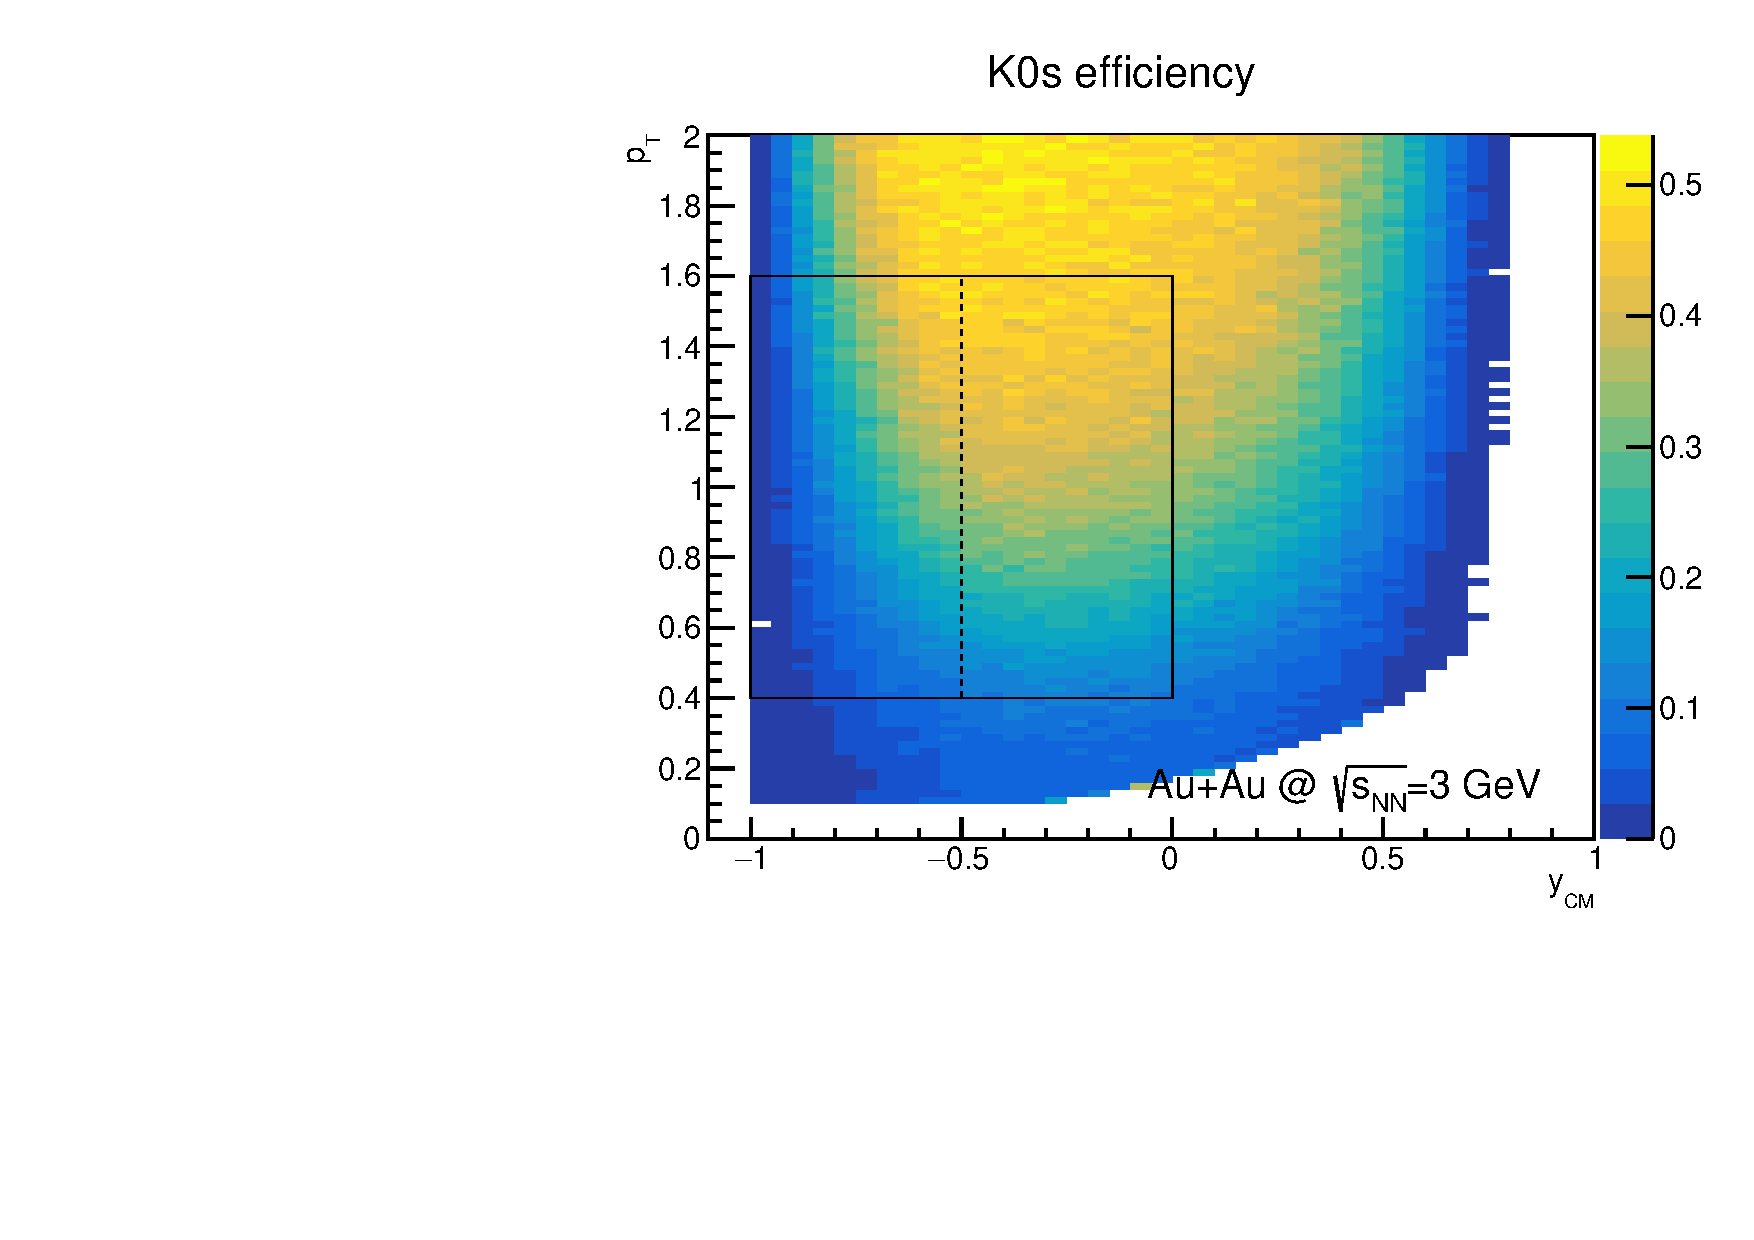
\includegraphics[width=0.45\linewidth]{figures/chapter02/3gev_K0s_eff.pdf}
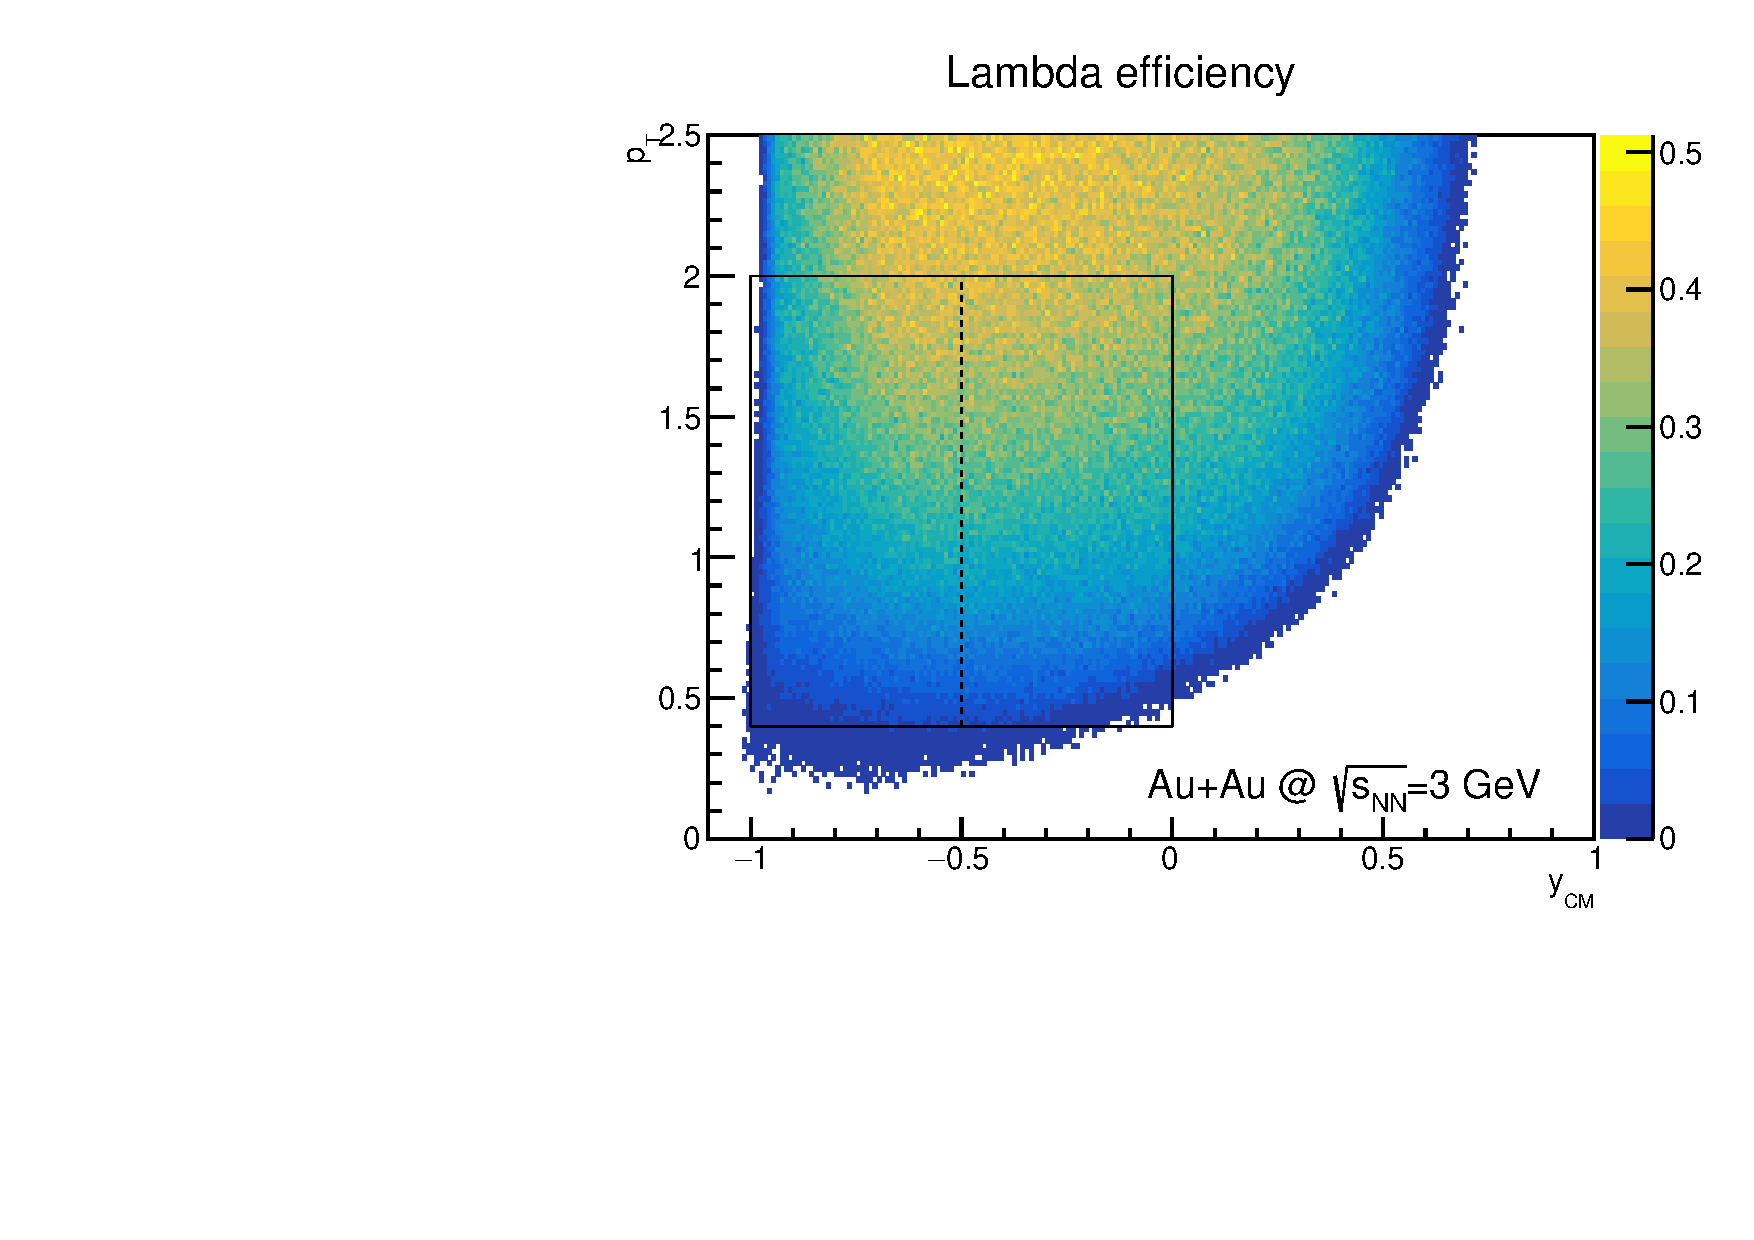
\includegraphics[width=0.45\linewidth]{figures/chapter02/3gev_lambda_eff.pdf}
\caption{Reconstruction efficiency of $K^{0}_{S}(Left), \Lambda(Right)$ as function of rapidity y and transverse momentum $p_T$ at $\sqrt{s_{NN}}$ = 3.0 GeV.}
\label{fig:3gev_K0sLam_eff}
\end{figure}

% Chapter 03
\section{$v_1$ plots for other energies}

\begin{figure}[hbt!]
\centering
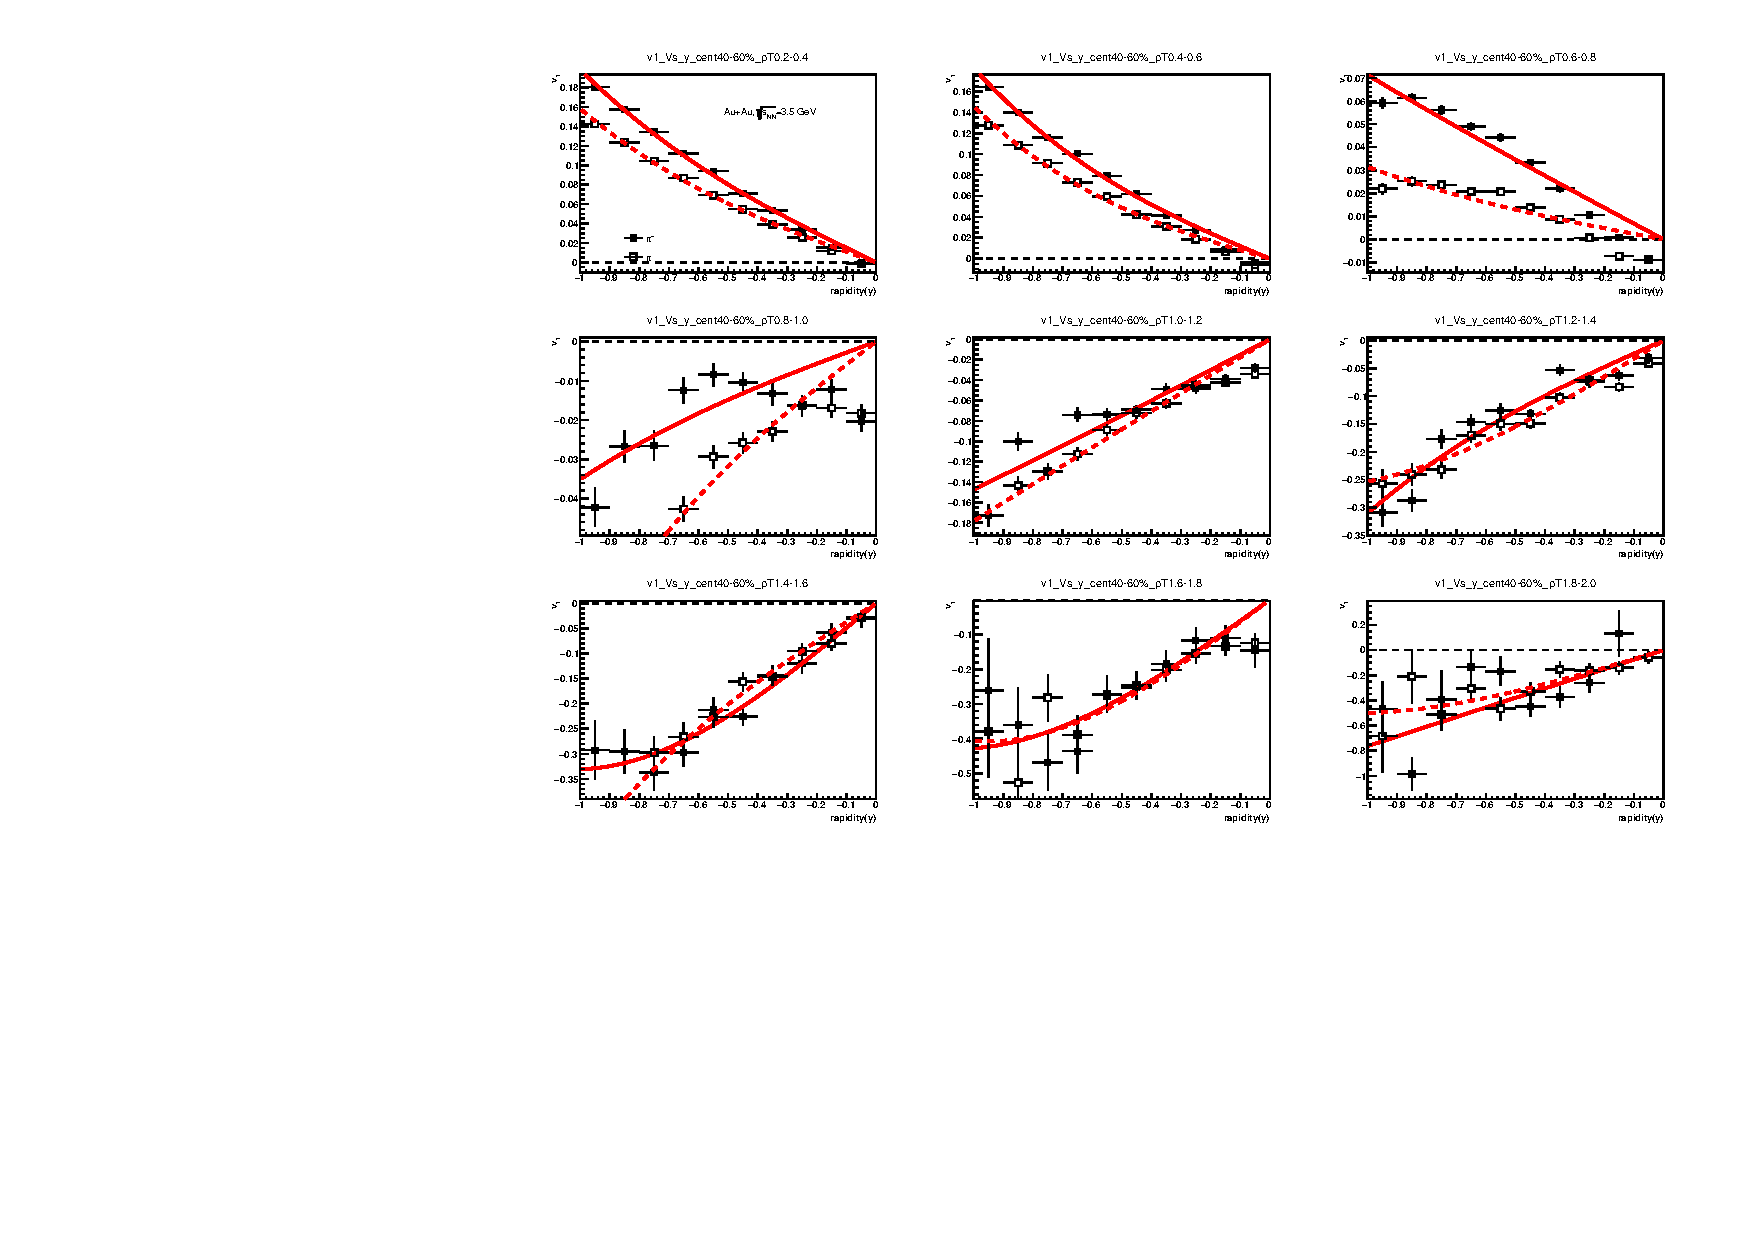
\includegraphics[width=0.85\linewidth]{figures/chapter03/3p5gev_pionp_v1VSy_9pT_cent0.pdf}
\caption{$v_1$ of pions as function of rapidity within $p_T$ windows in 40-60\% centrality at $\sqrt{s_{NN}}$ = 3.5 GeV.}
\label{fig:3p5gev_pion_v1y_pt_cent0}
\end{figure}

\begin{figure}[hbt!]
\centering
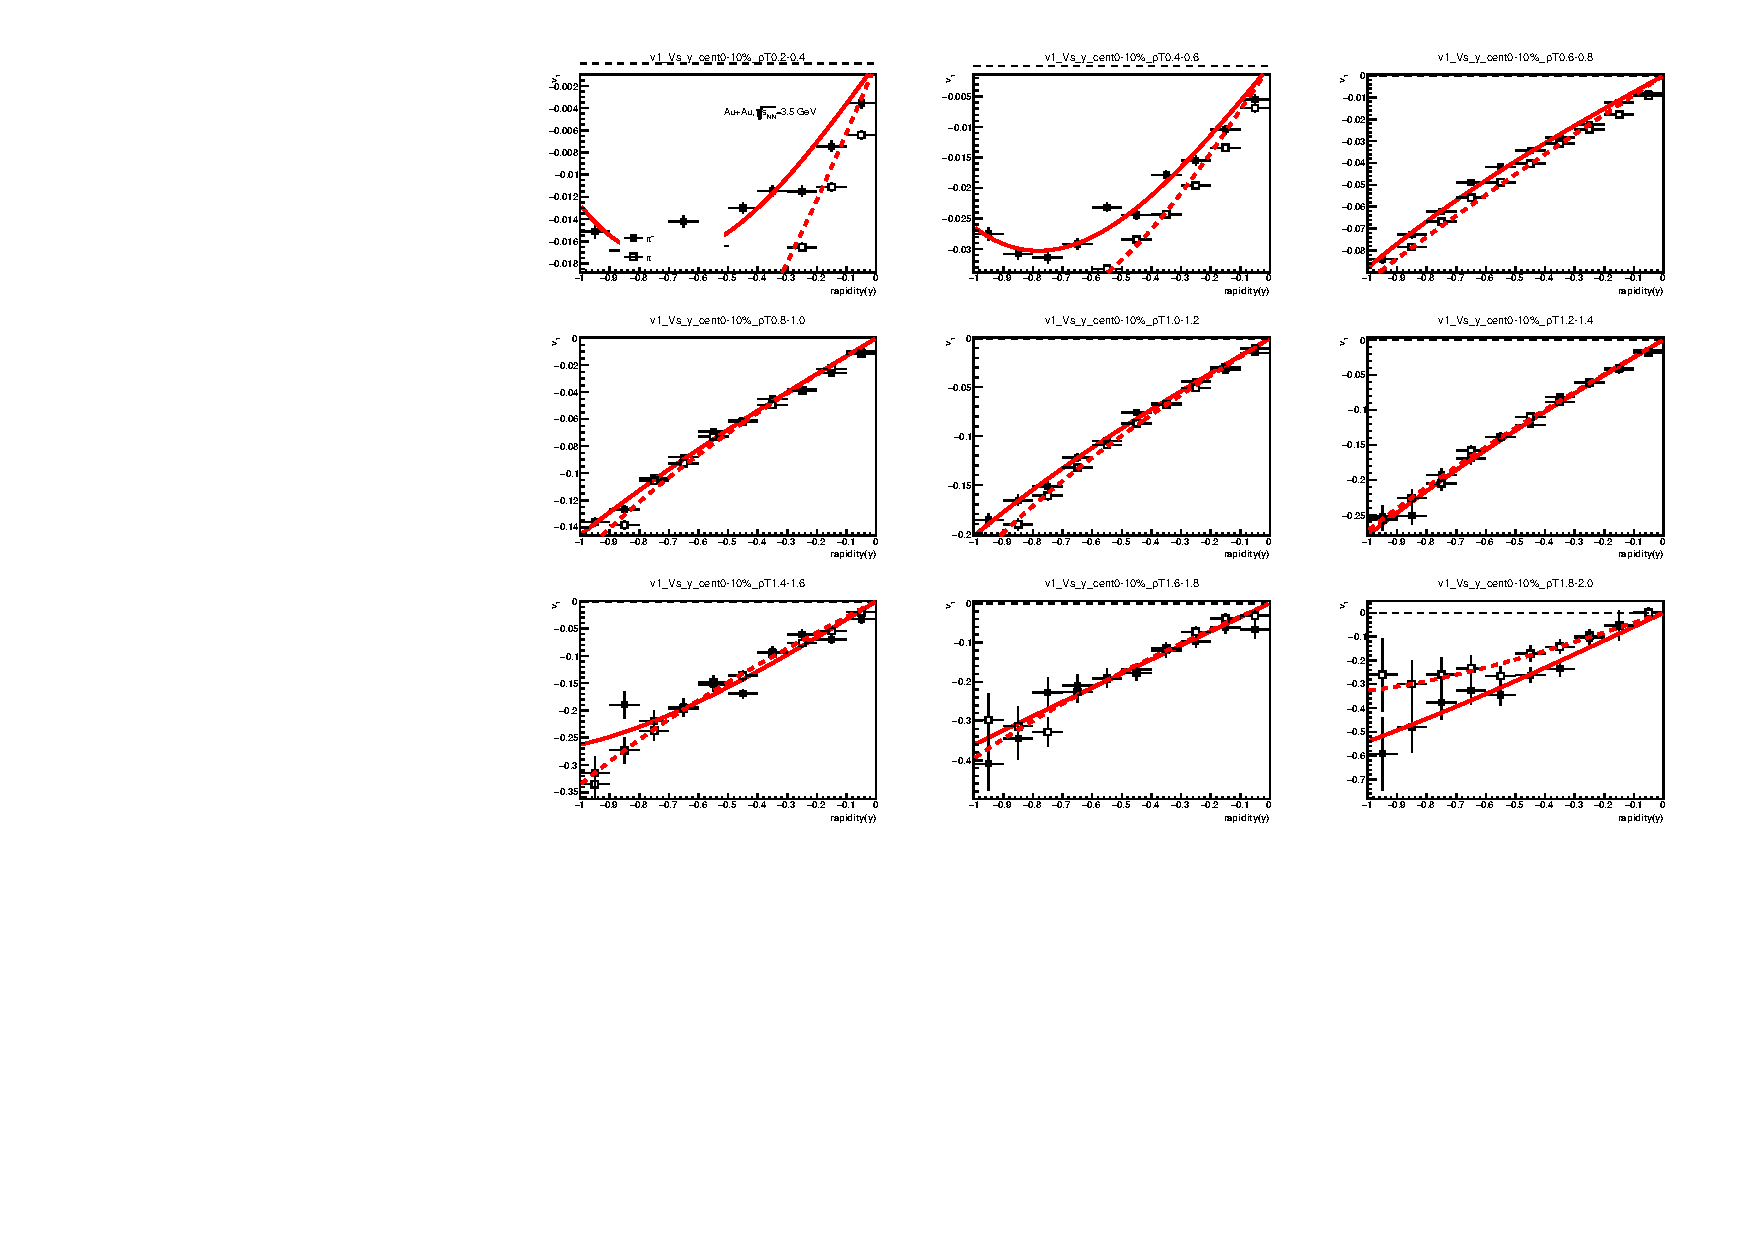
\includegraphics[width=0.85\linewidth]{figures/chapter03/3p5gev_pionp_v1VSy_9pT_cent2.pdf}
\caption{$v_1$ of pions as function of rapidity within $p_T$ windows in 0-10\% centrality at $\sqrt{s_{NN}}$ = 3.5 GeV.}
\label{fig:3p5gev_pion_v1y_pt_cent2}
\end{figure}


\begin{figure}[hbt!]
\centering
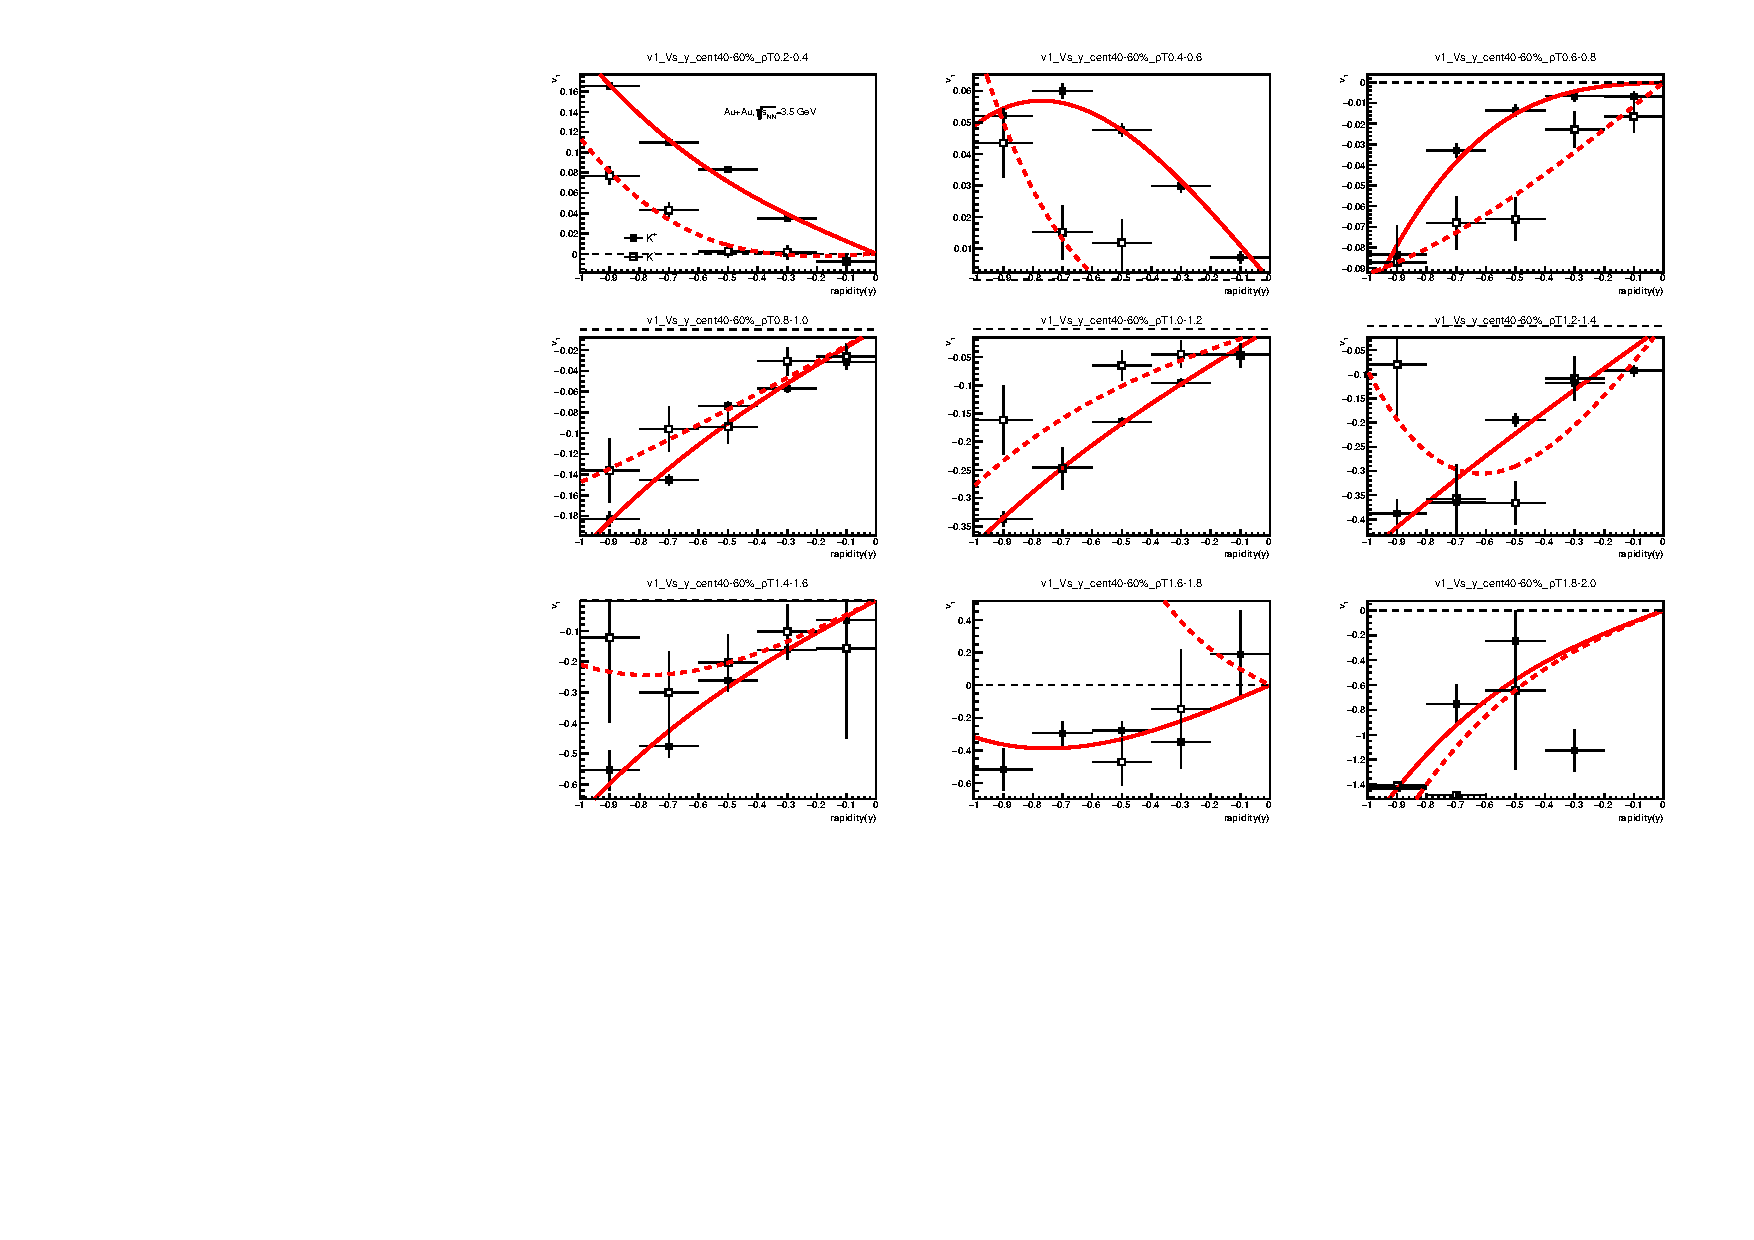
\includegraphics[width=0.85\linewidth]{figures/chapter03/3p5gev_kaonp_v1VSy_9pT_cent0.pdf}
\caption{$v_1$ of kaons as function of rapidity within $p_T$ windows in 40-60\% centrality at $\sqrt{s_{NN}}$ = 3.5 GeV.}
\label{fig:3p5gev_kaon_v1y_pt_cent0}
\end{figure}

\begin{figure}[hbt!]
\centering
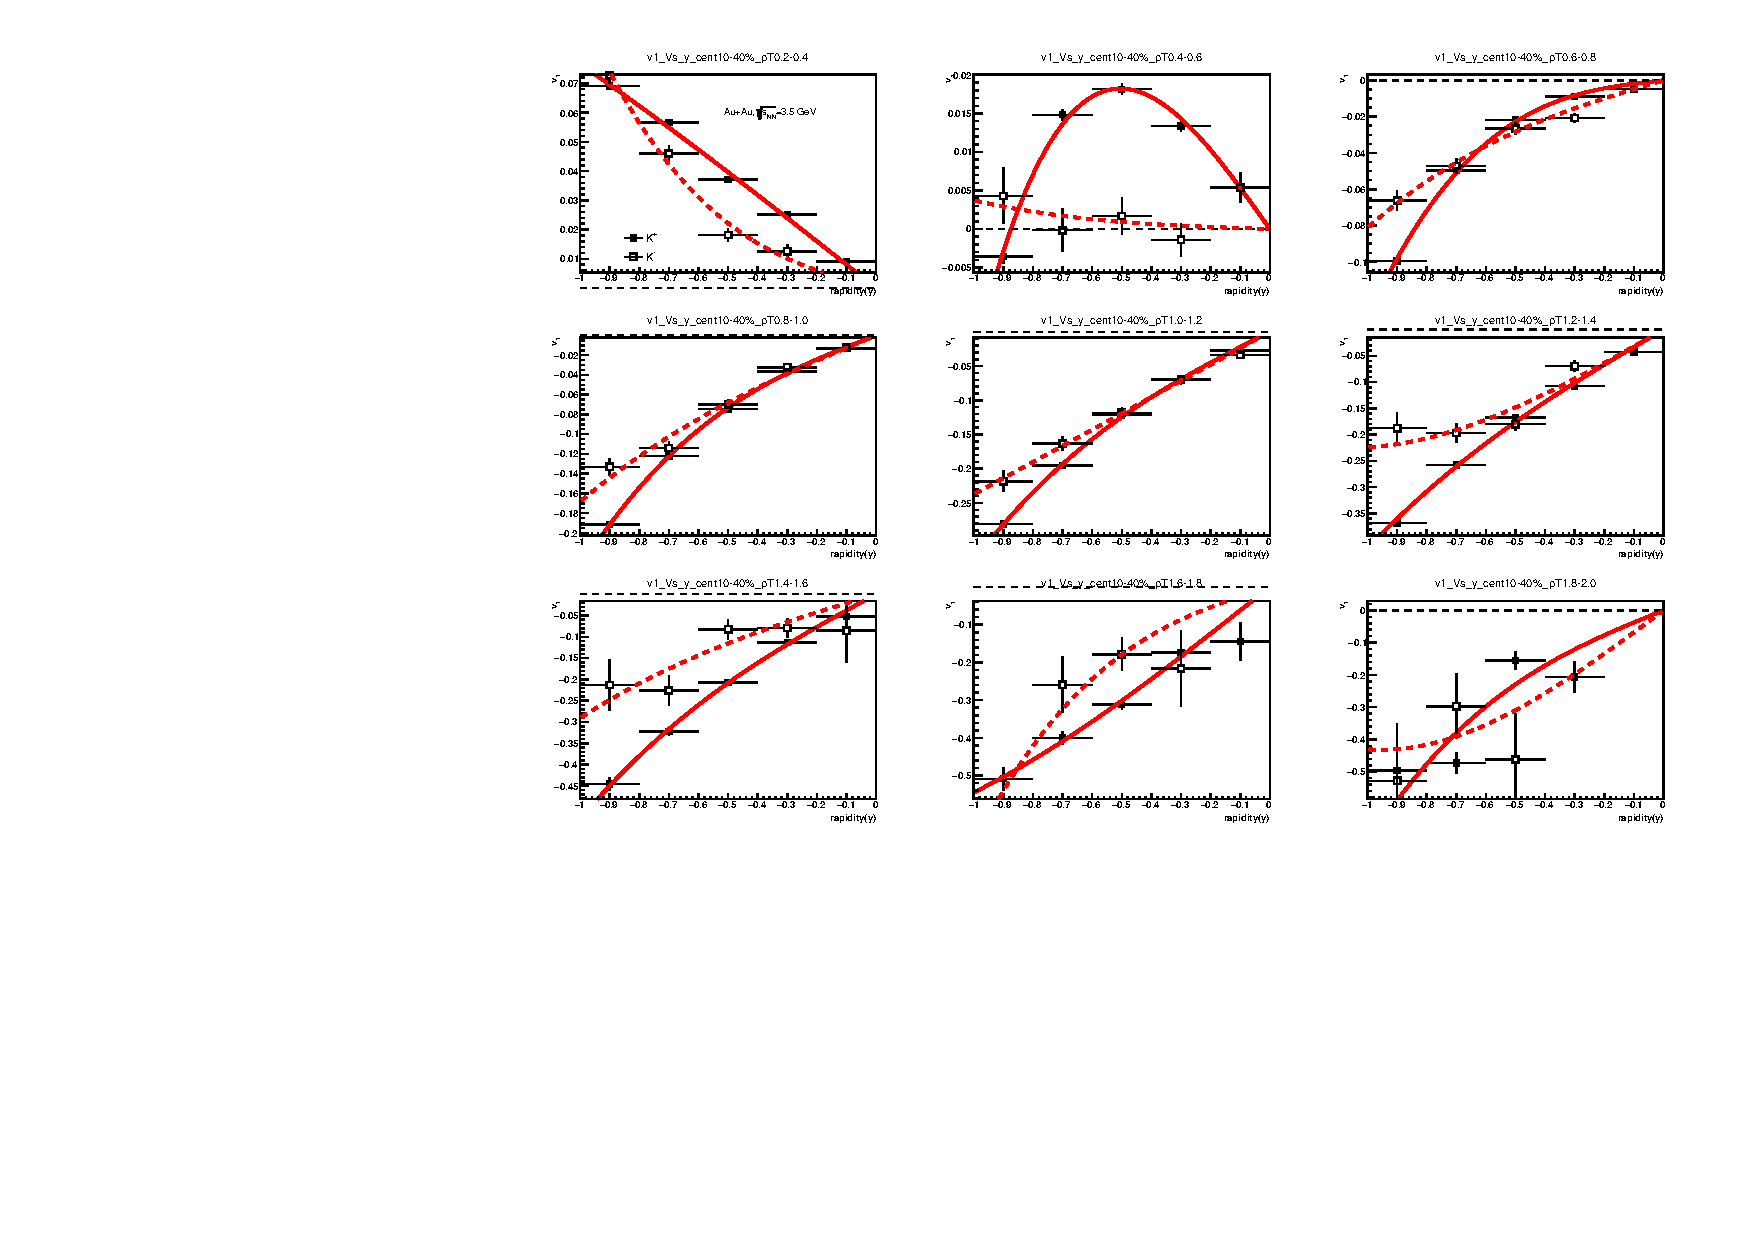
\includegraphics[width=0.85\linewidth]{figures/chapter03/3p5gev_kaonp_v1VSy_9pT_cent1.pdf}
\caption{$v_1$ of kaons as function of rapidity within $p_T$ windows in 10-40\% centrality at $\sqrt{s_{NN}}$ = 3.5 GeV.}
\label{fig:3p5gev_kaon_v1y_pt_cent1}
\end{figure}
    
\begin{figure}[hbt!]
\centering
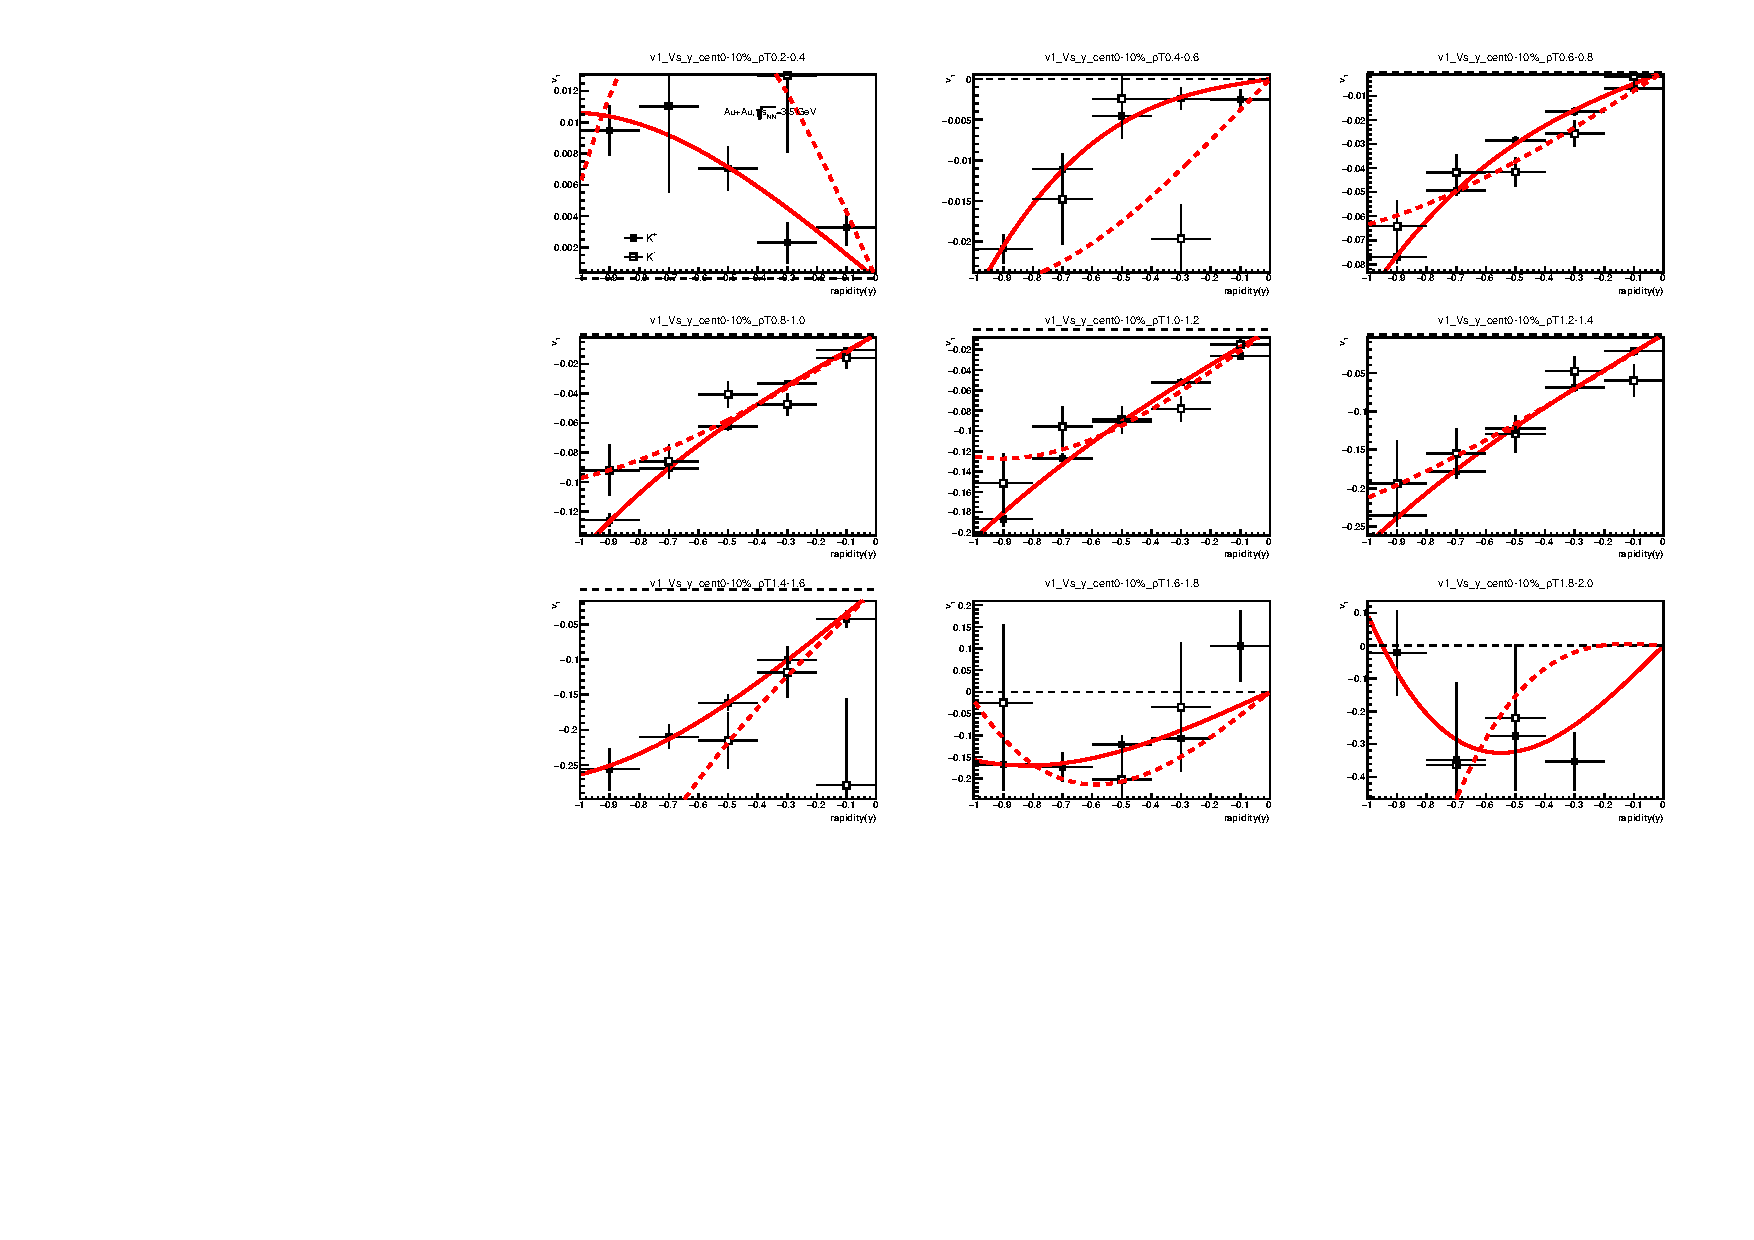
\includegraphics[width=0.85\linewidth]{figures/chapter03/3p5gev_kaonp_v1VSy_9pT_cent2.pdf}
\caption{$v_1$ of kaons as function of rapidity within $p_T$ windows in 0-10\% centrality at $\sqrt{s_{NN}}$ = 3.5 GeV.}
\label{fig:3p5gev_kaon_v1y_pt_cent2}
\end{figure}

\begin{figure}[hbt!]
\centering
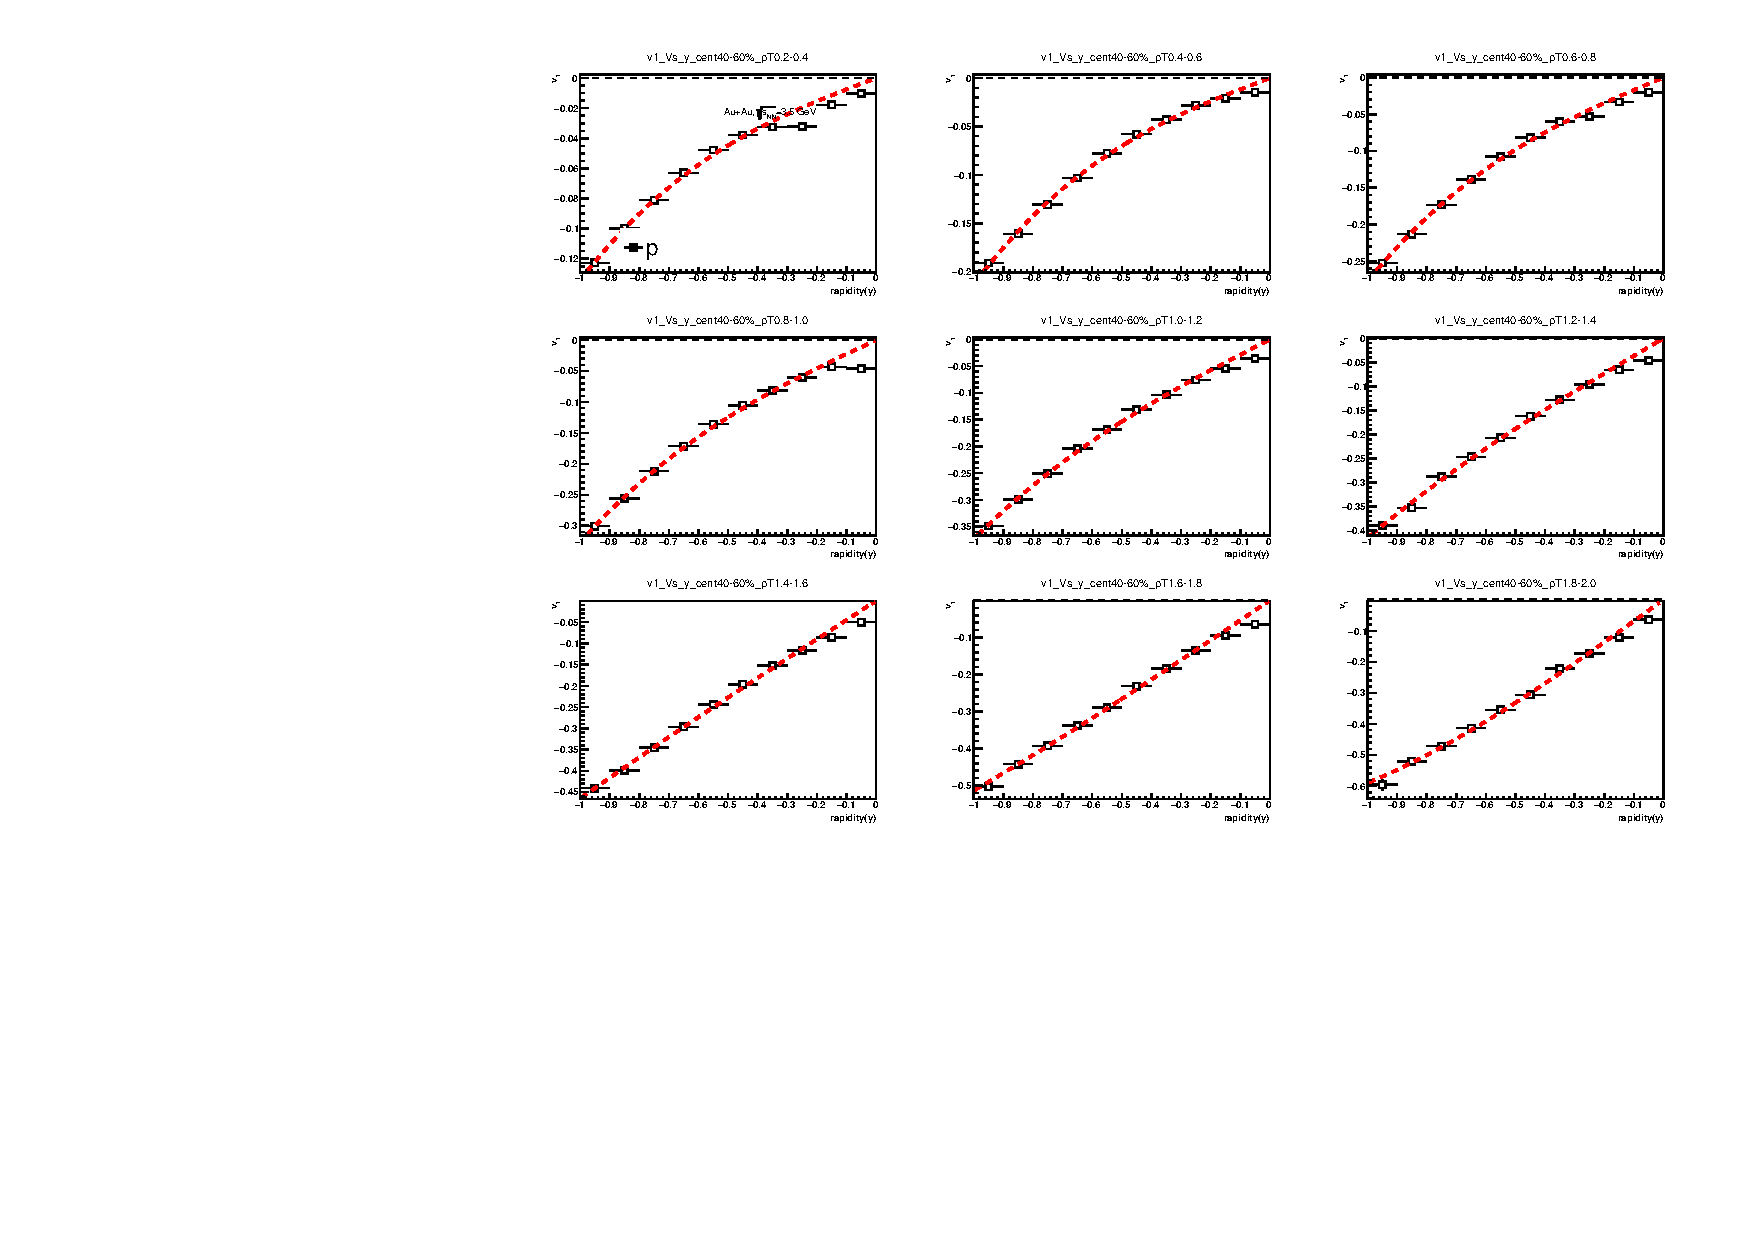
\includegraphics[width=0.85\linewidth]{figures/chapter03/3p5gev_protonp_v1VSy_9pT_cent0.pdf}
\caption{$v_1$ of proton as function of rapidity within $p_T$ windows in 40-60\% centrality at $\sqrt{s_{NN}}$ = 3.5 GeV.}
\label{fig:3p5gev_proton_v1y_pt_cent0}
\end{figure}
    
\begin{figure}[hbt!]
\centering
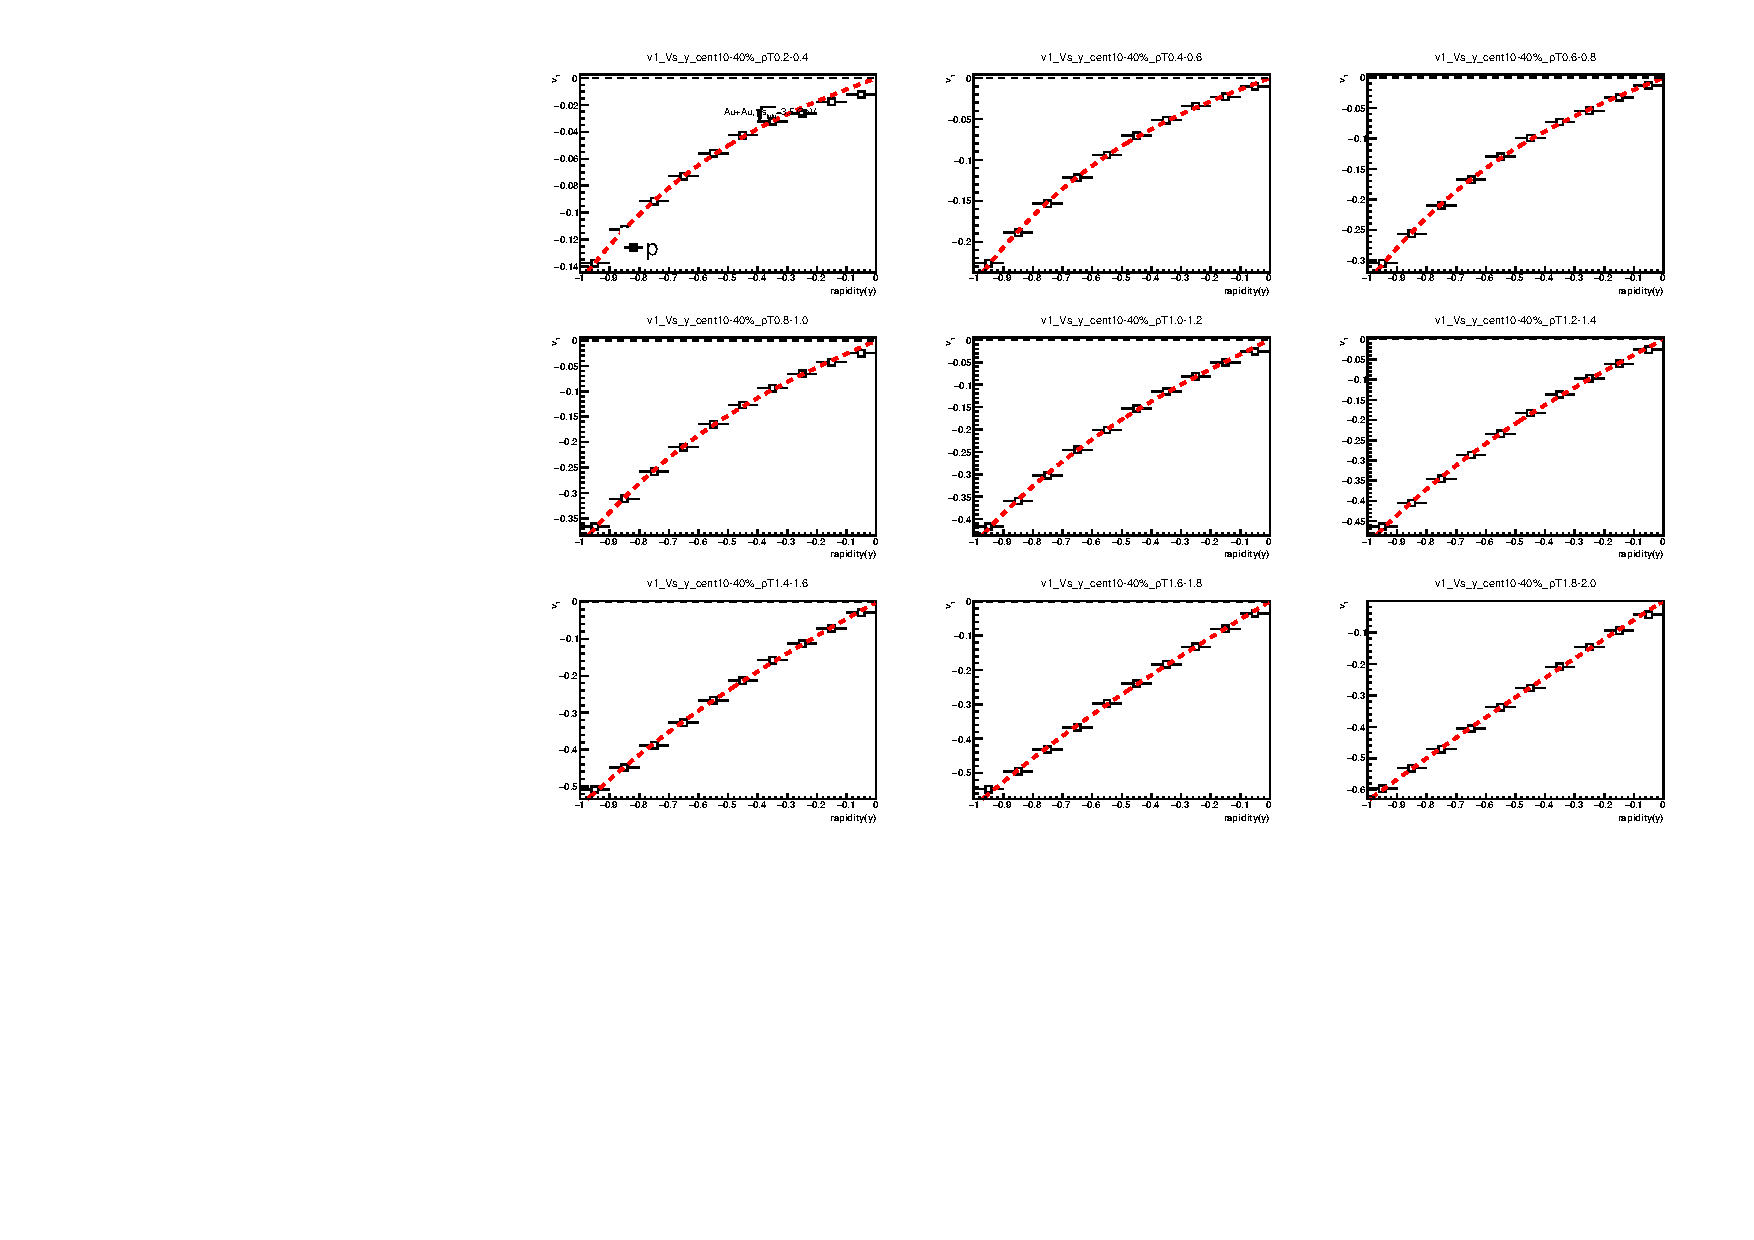
\includegraphics[width=0.85\linewidth]{figures/chapter03/3p5gev_protonp_v1VSy_9pT_cent1.pdf}
\caption{$v_1$ of proton as function of rapidity within $p_T$ windows in 10-40\% centrality at $\sqrt{s_{NN}}$ = 3.5 GeV.}
\label{fig:3p5gev_proton_v1y_pt_cent1}
\end{figure}
        
\begin{figure}[hbt!]
\centering
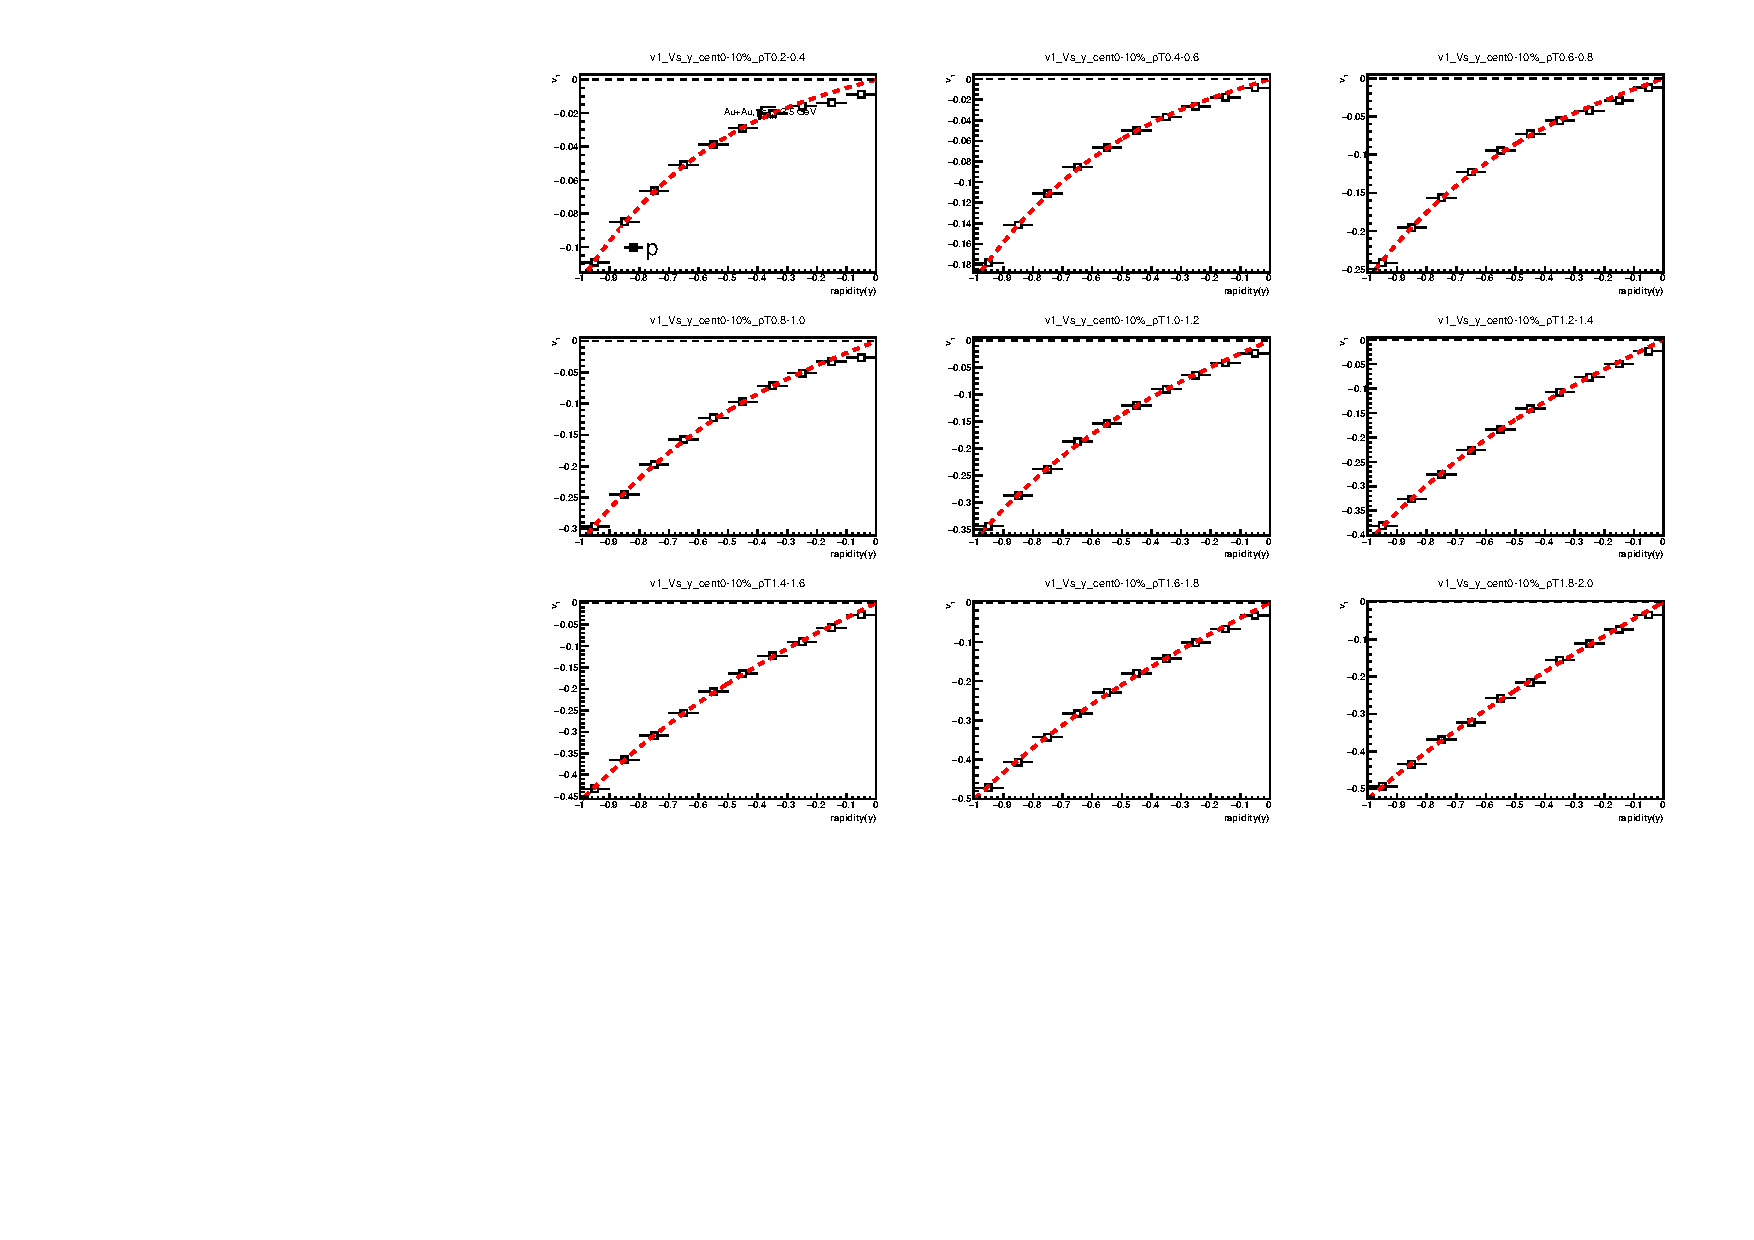
\includegraphics[width=0.85\linewidth]{figures/chapter03/3p5gev_protonp_v1VSy_9pT_cent2.pdf}
\caption{$v_1$ of proton as function of rapidity within $p_T$ windows in 0-10\% centrality at $\sqrt{s_{NN}}$ = 3.5 GeV.}
\label{fig:3p5gev_proton_v1y_pt_cent2}
\end{figure}

\begin{figure}[hbt!]
\centering
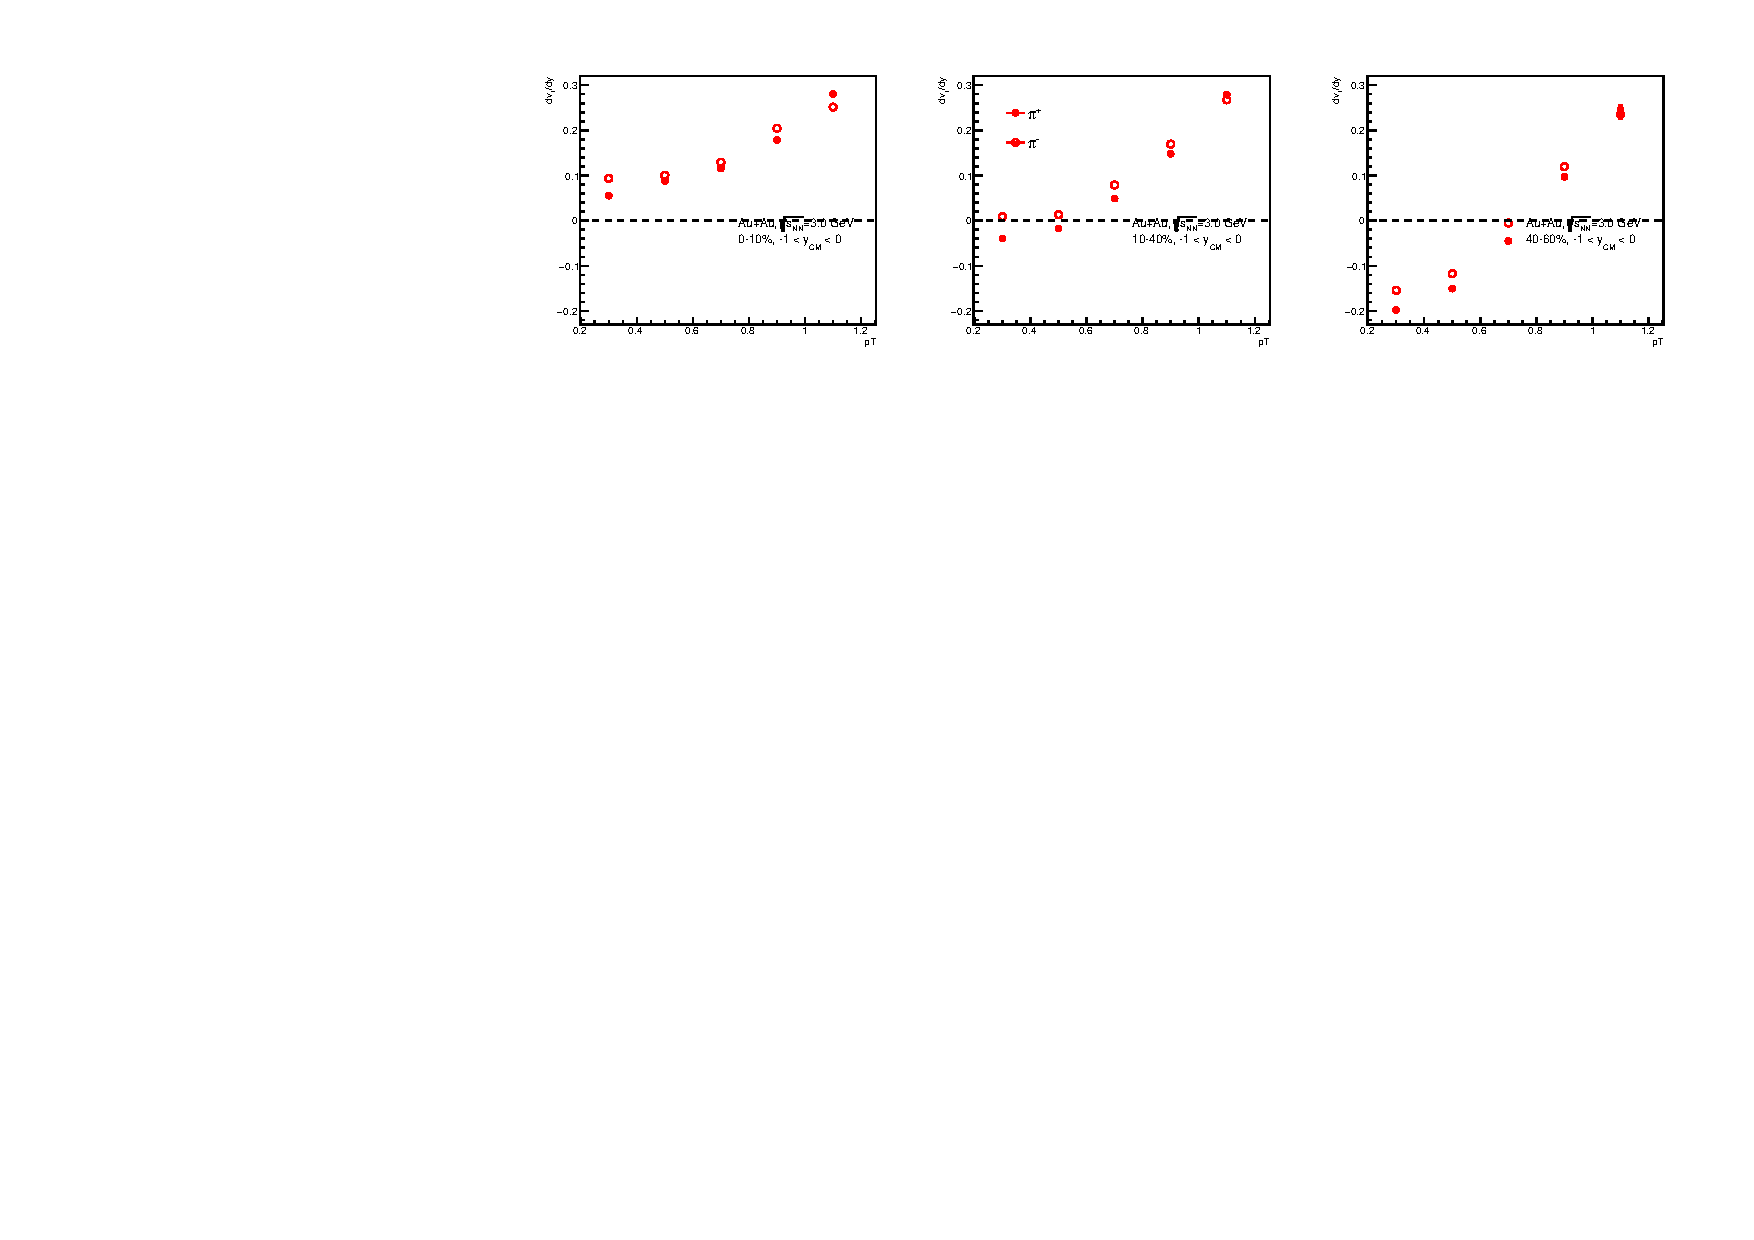
\includegraphics[width=0.95\linewidth]{figures/chapter03/3gev_pionp_v1Slope_pT.pdf}
\caption{$dv_1/dy|_{y=0}$ of pions as function of $p_T$ at $\sqrt{s_{NN}}$ = 3.0 GeV.}
\label{fig:3gev_pion_v1Slope_pt}
\end{figure}

\begin{figure}[hbt!]
\centering
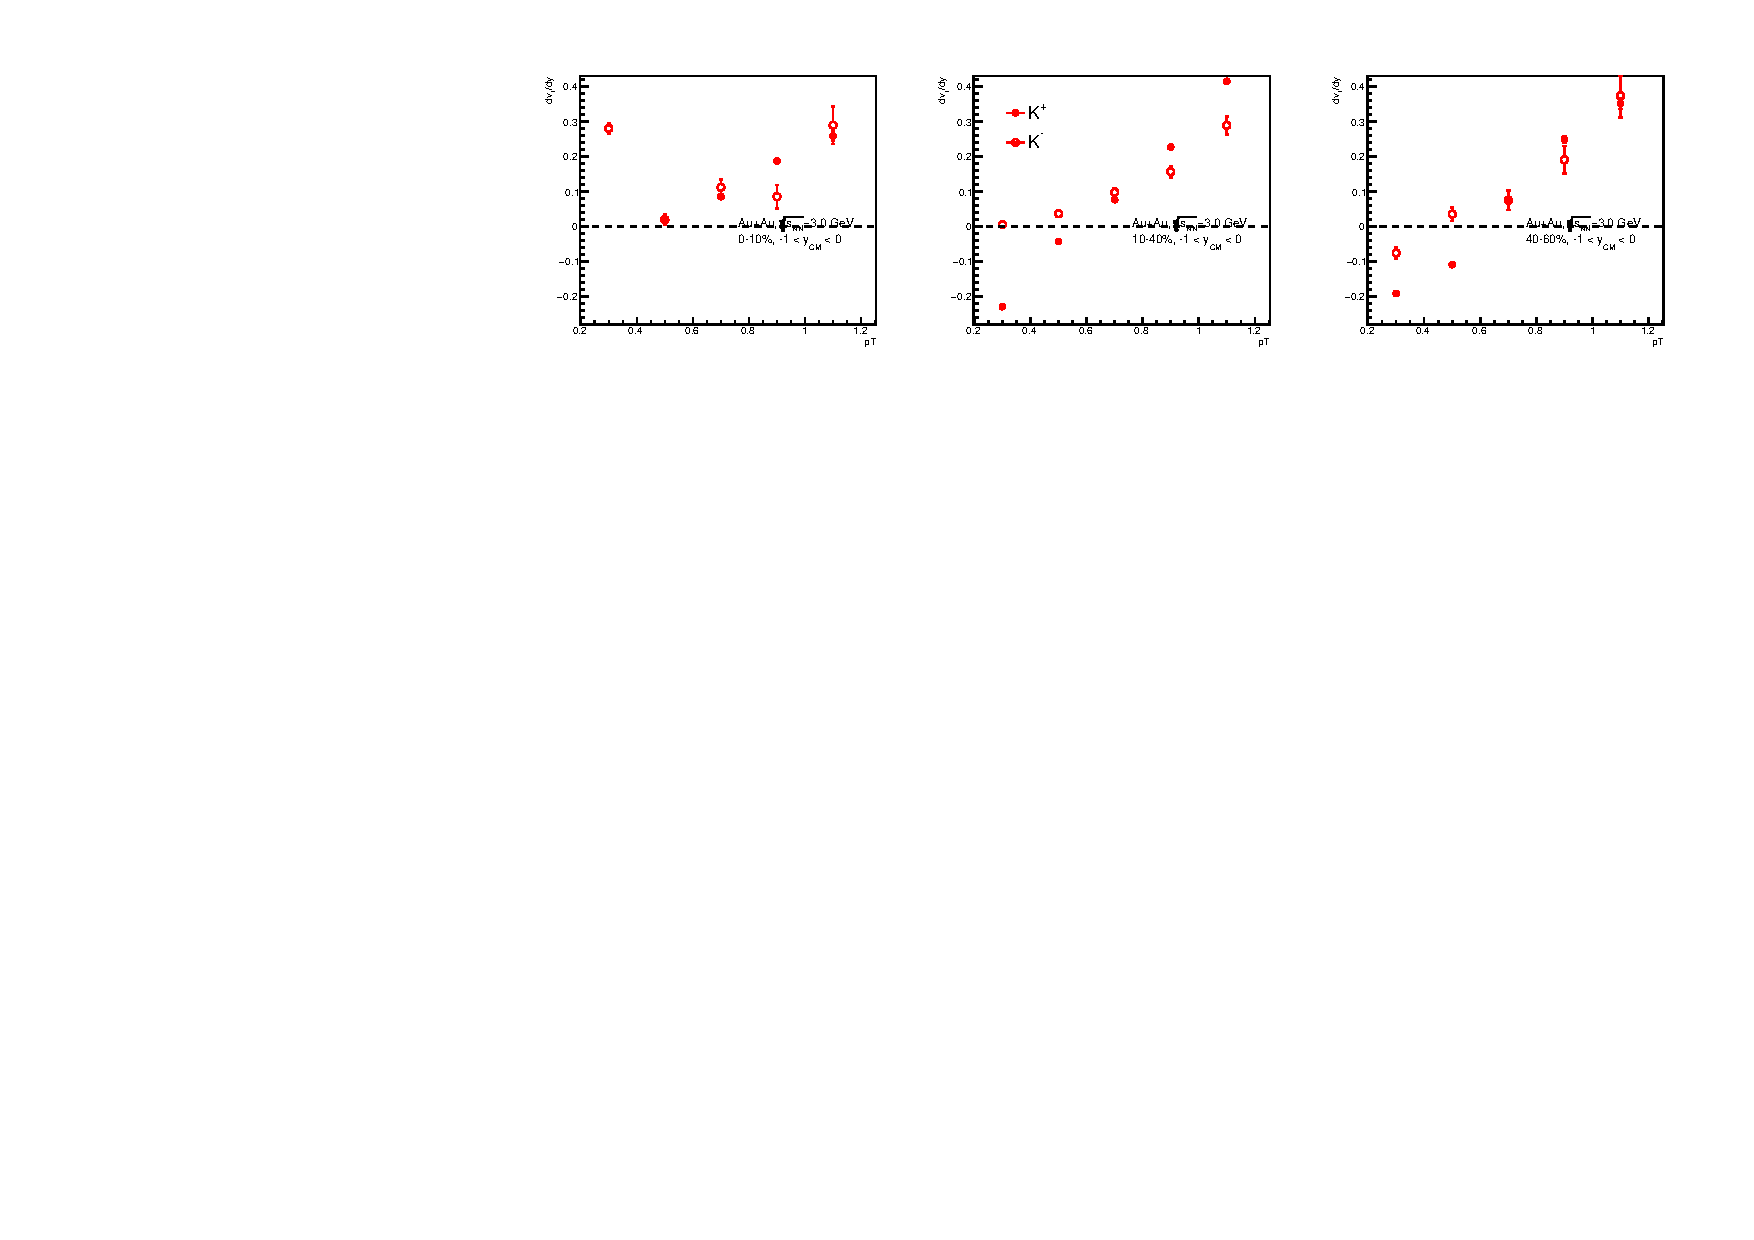
\includegraphics[width=0.95\linewidth]{figures/chapter03/3gev_kaonp_v1Slope_pT.pdf}
\caption{$dv_1/dy|_{y=0}$ of kaons as function of $p_T$ at $\sqrt{s_{NN}}$ = 3.0 GeV.}
\label{fig:3gev_kaon_v1Slope_pt}
\end{figure}

\begin{figure}[hbt!]
\centering
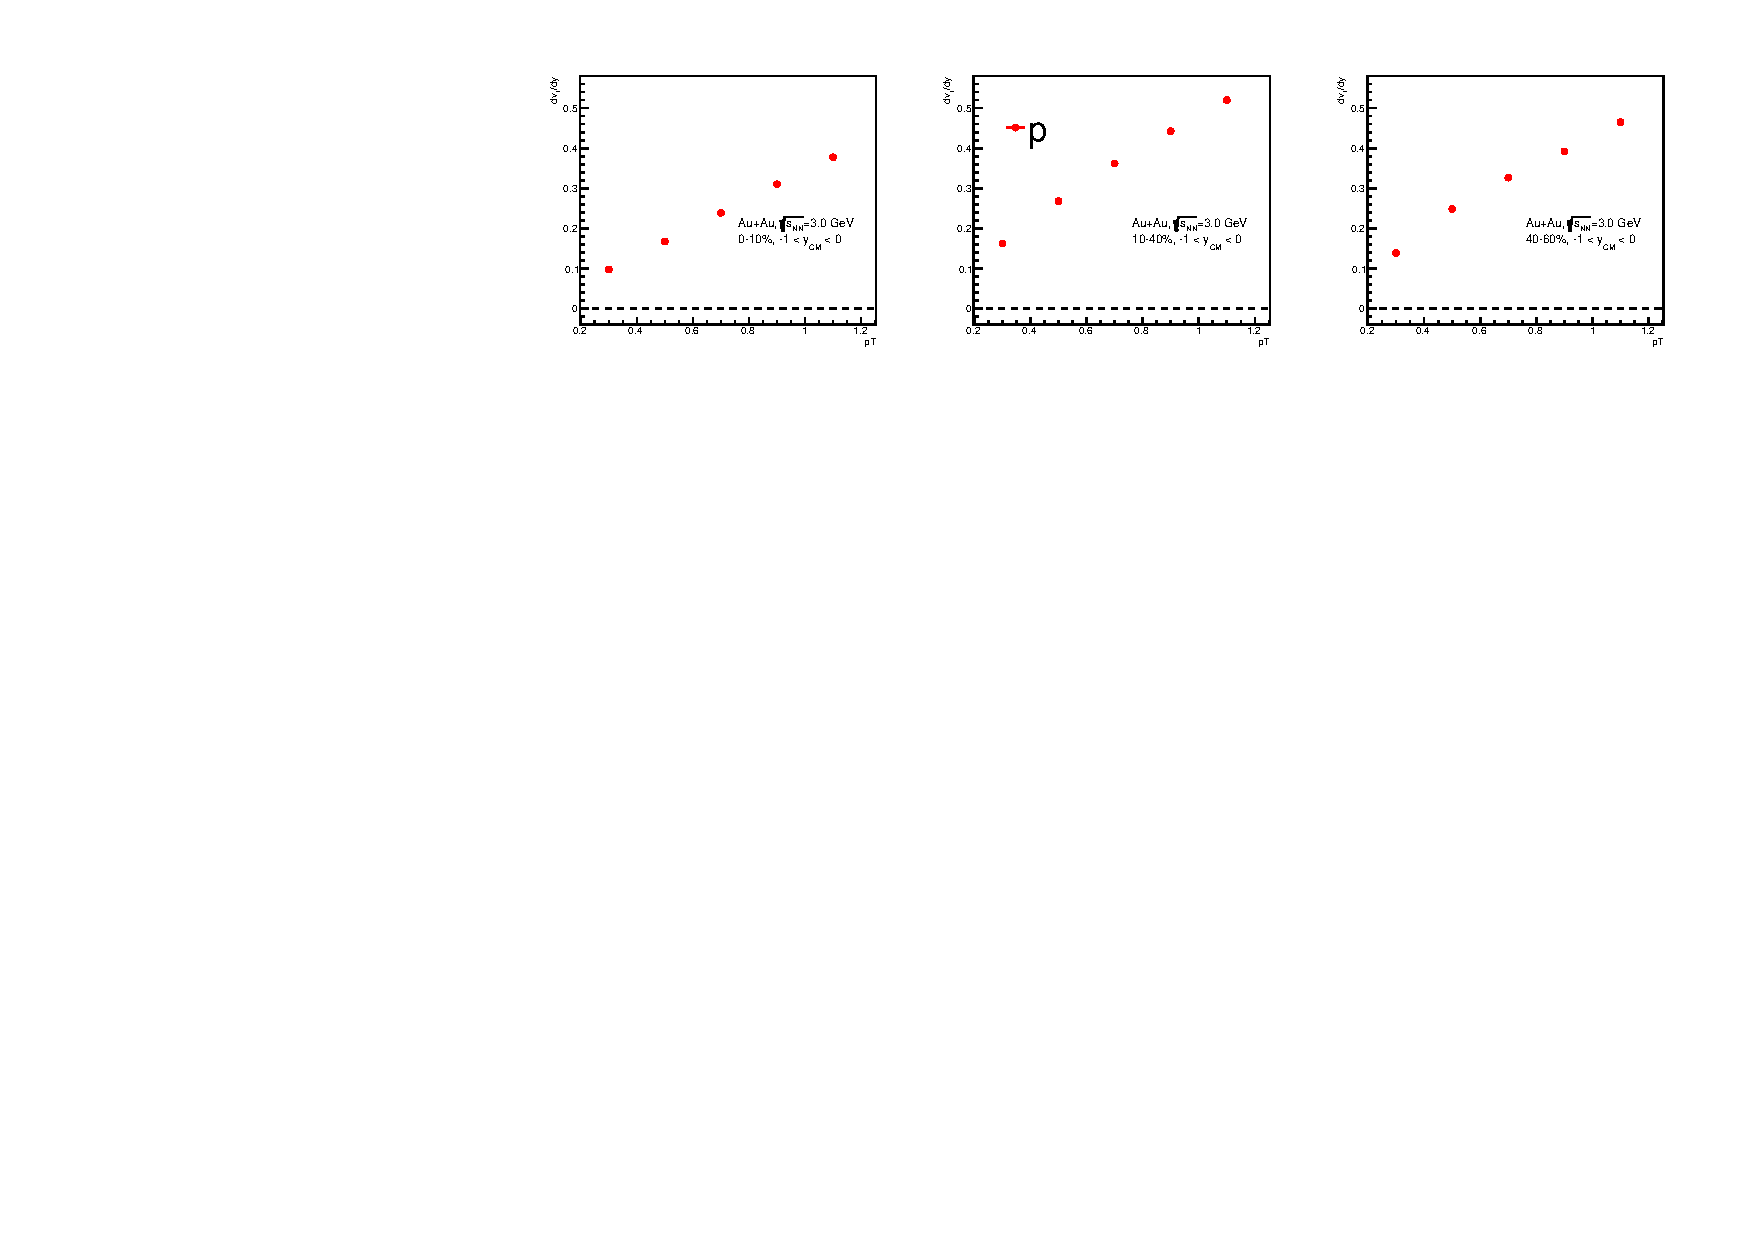
\includegraphics[width=0.95\linewidth]{figures/chapter03/3gev_protonp_v1Slope_pT.pdf}
\caption{$dv_1/dy|_{y=0}$ of proton as function of $p_T$ at $\sqrt{s_{NN}}$ = 3.0 GeV.}
\label{fig:3gev_proton_v1Slope_pt}
\end{figure}

\begin{figure}[hbt!]
\centering
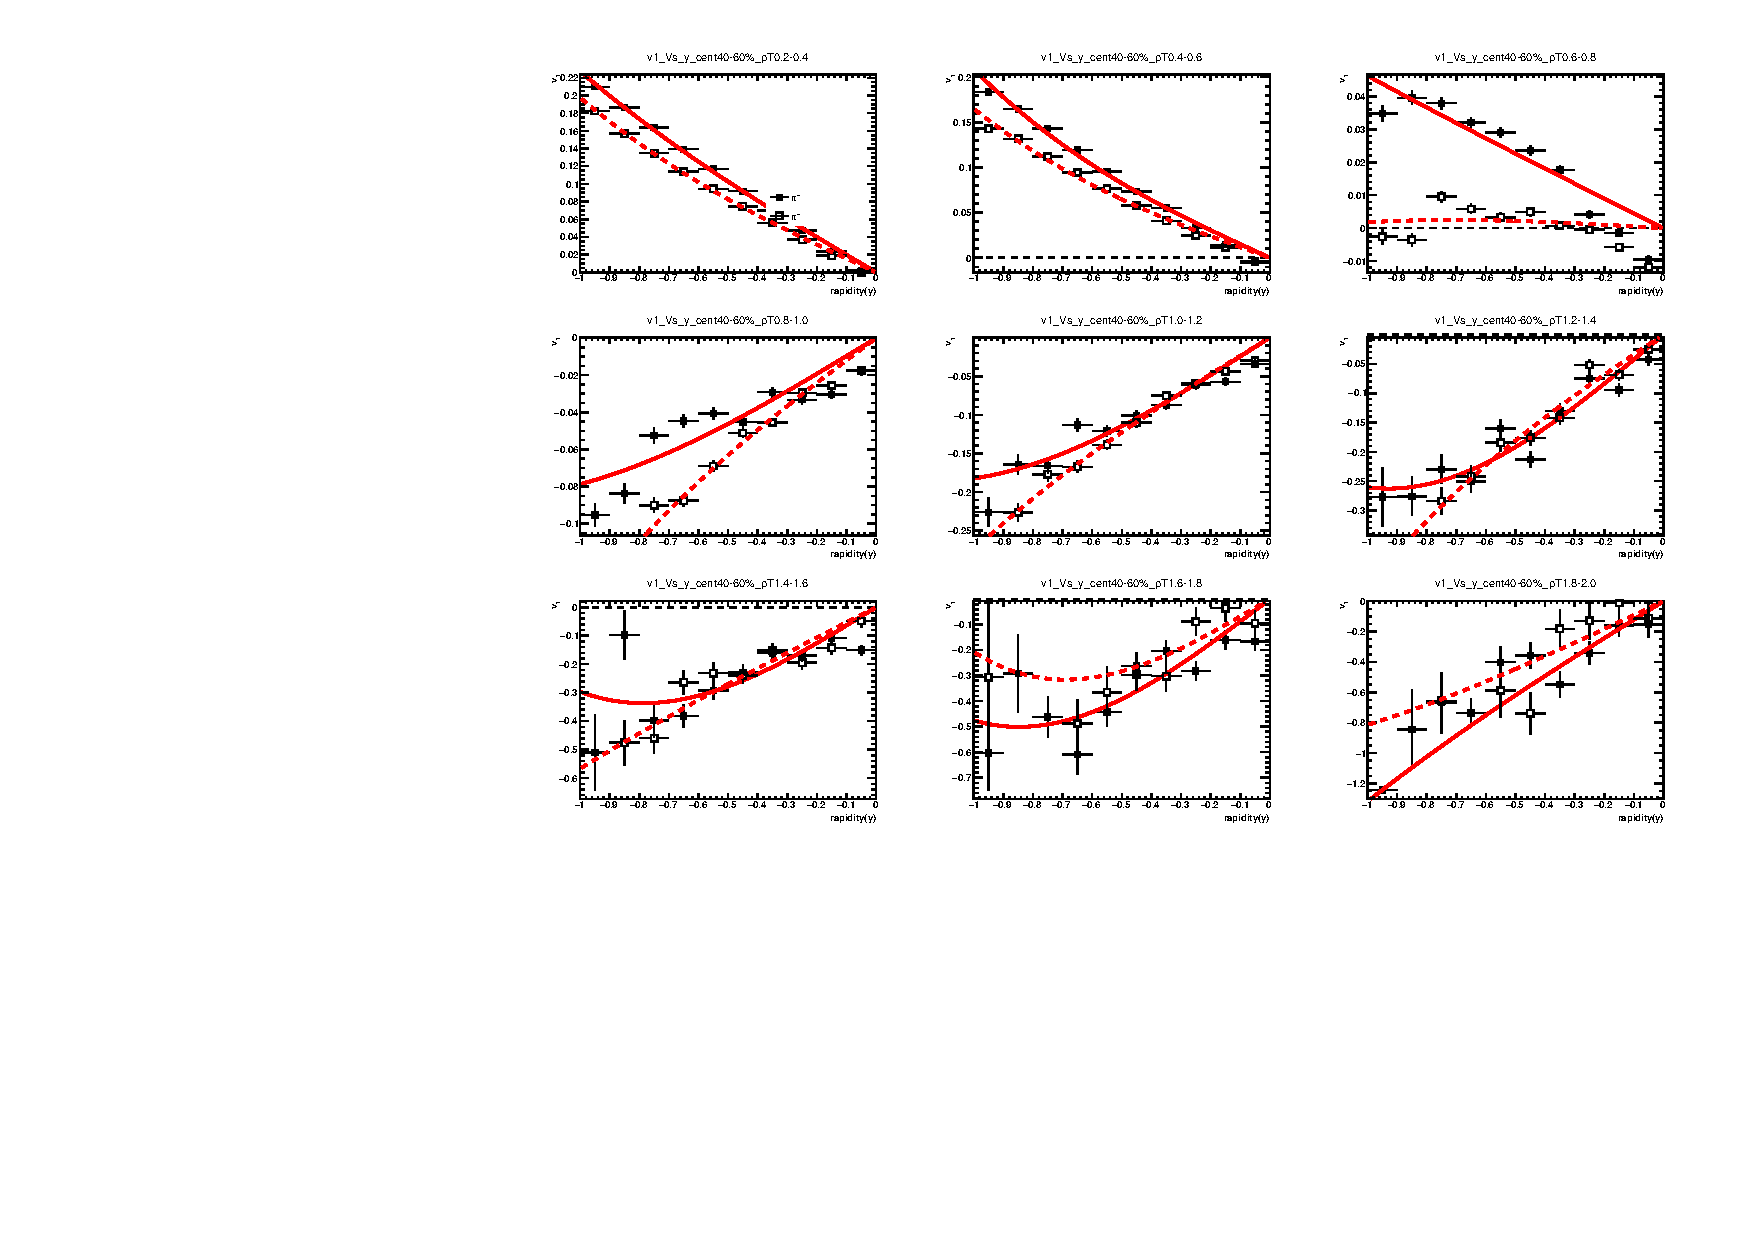
\includegraphics[width=0.85\linewidth]{figures/chapter03/3gev_pionp_v1VSy_9pT_cent0.pdf}
\caption{$v_1$ of pions as function of rapidity within $p_T$ windows in 40-60\% centrality at $\sqrt{s_{NN}}$ = 3.0 GeV.}
\label{fig:3gev_pion_v1y_pt_cent0}
\end{figure}
    
\begin{figure}[hbt!]
\centering
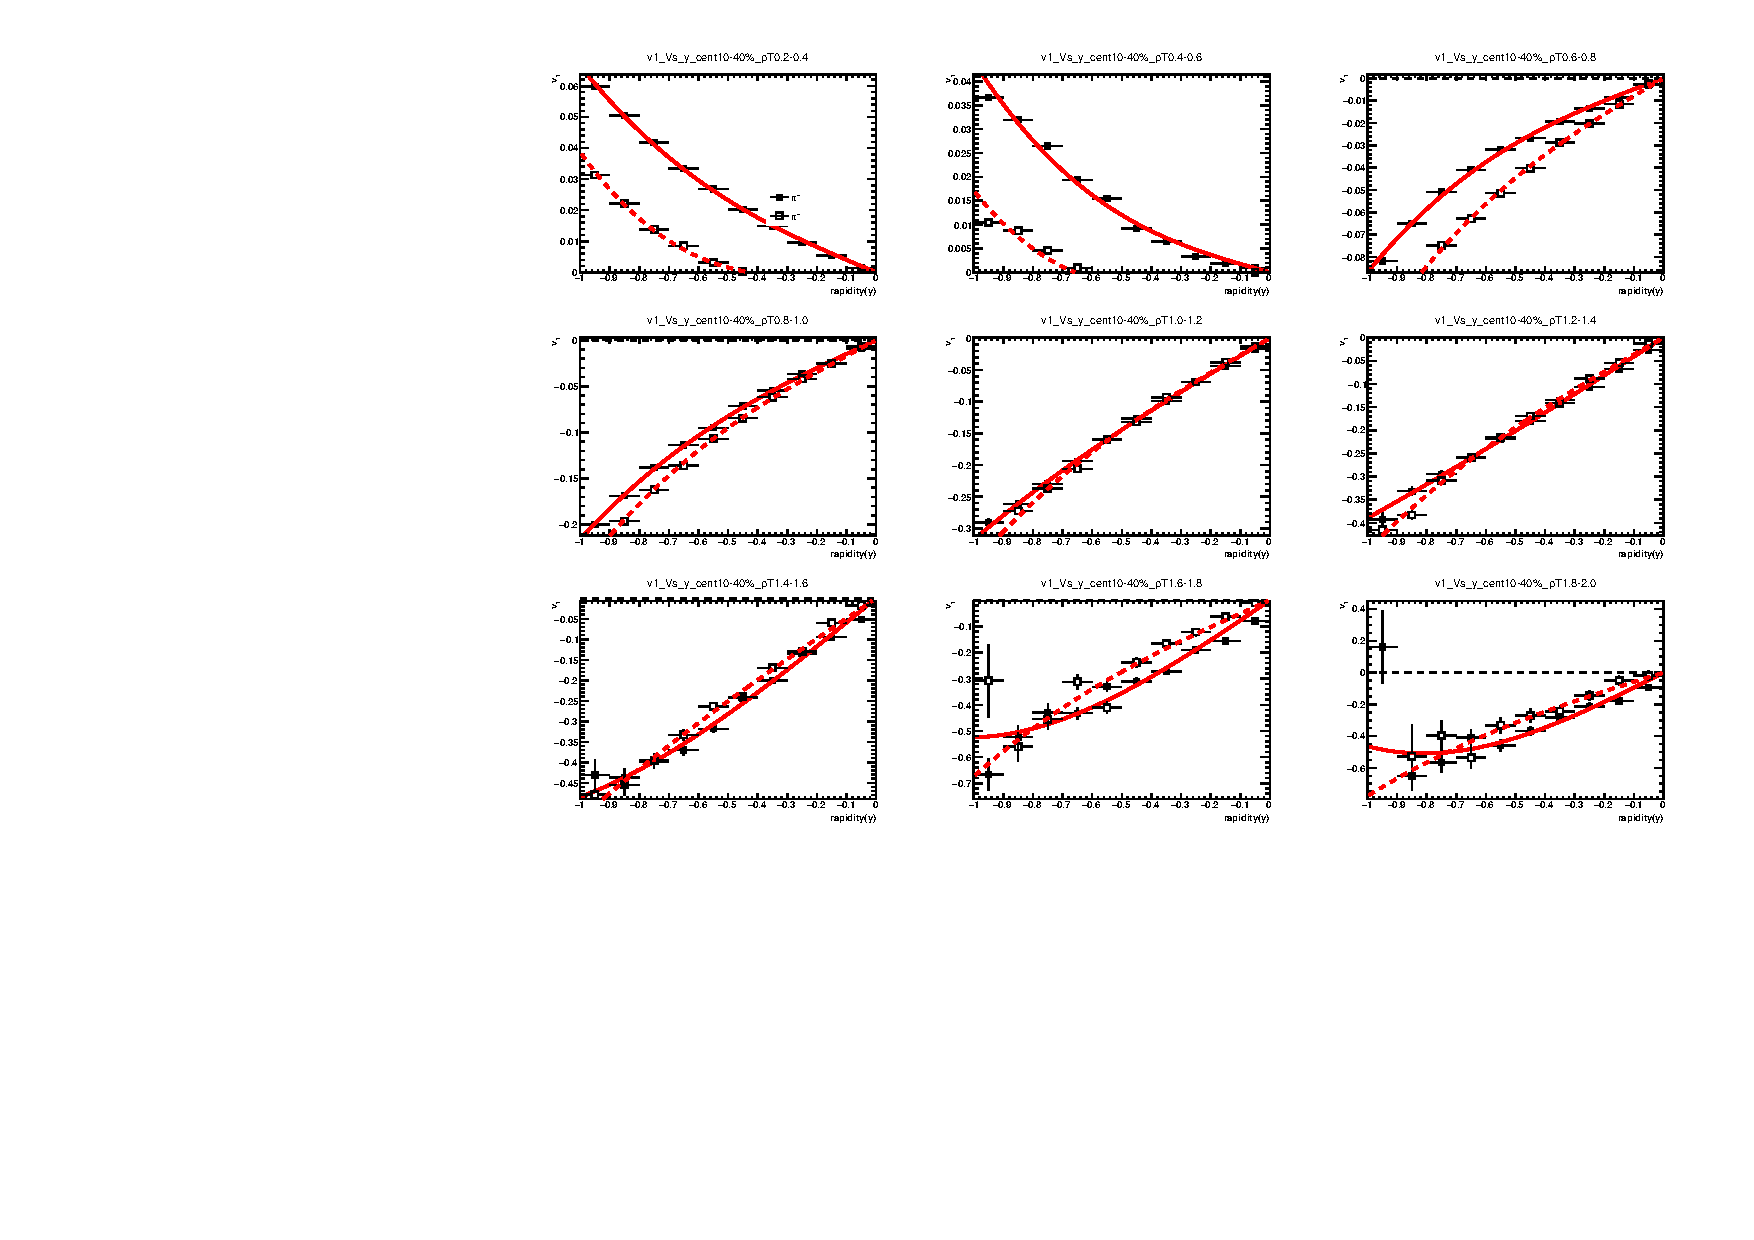
\includegraphics[width=0.85\linewidth]{figures/chapter03/3gev_pionp_v1VSy_9pT_cent1.pdf}
\caption{$v_1$ of pions as function of rapidity within $p_T$ windows in 10-40\% centrality at $\sqrt{s_{NN}}$ = 3.0 GeV.}
\label{fig:3gev_pion_v1y_pt_cent1}
\end{figure}
        
\begin{figure}[hbt!]
\centering
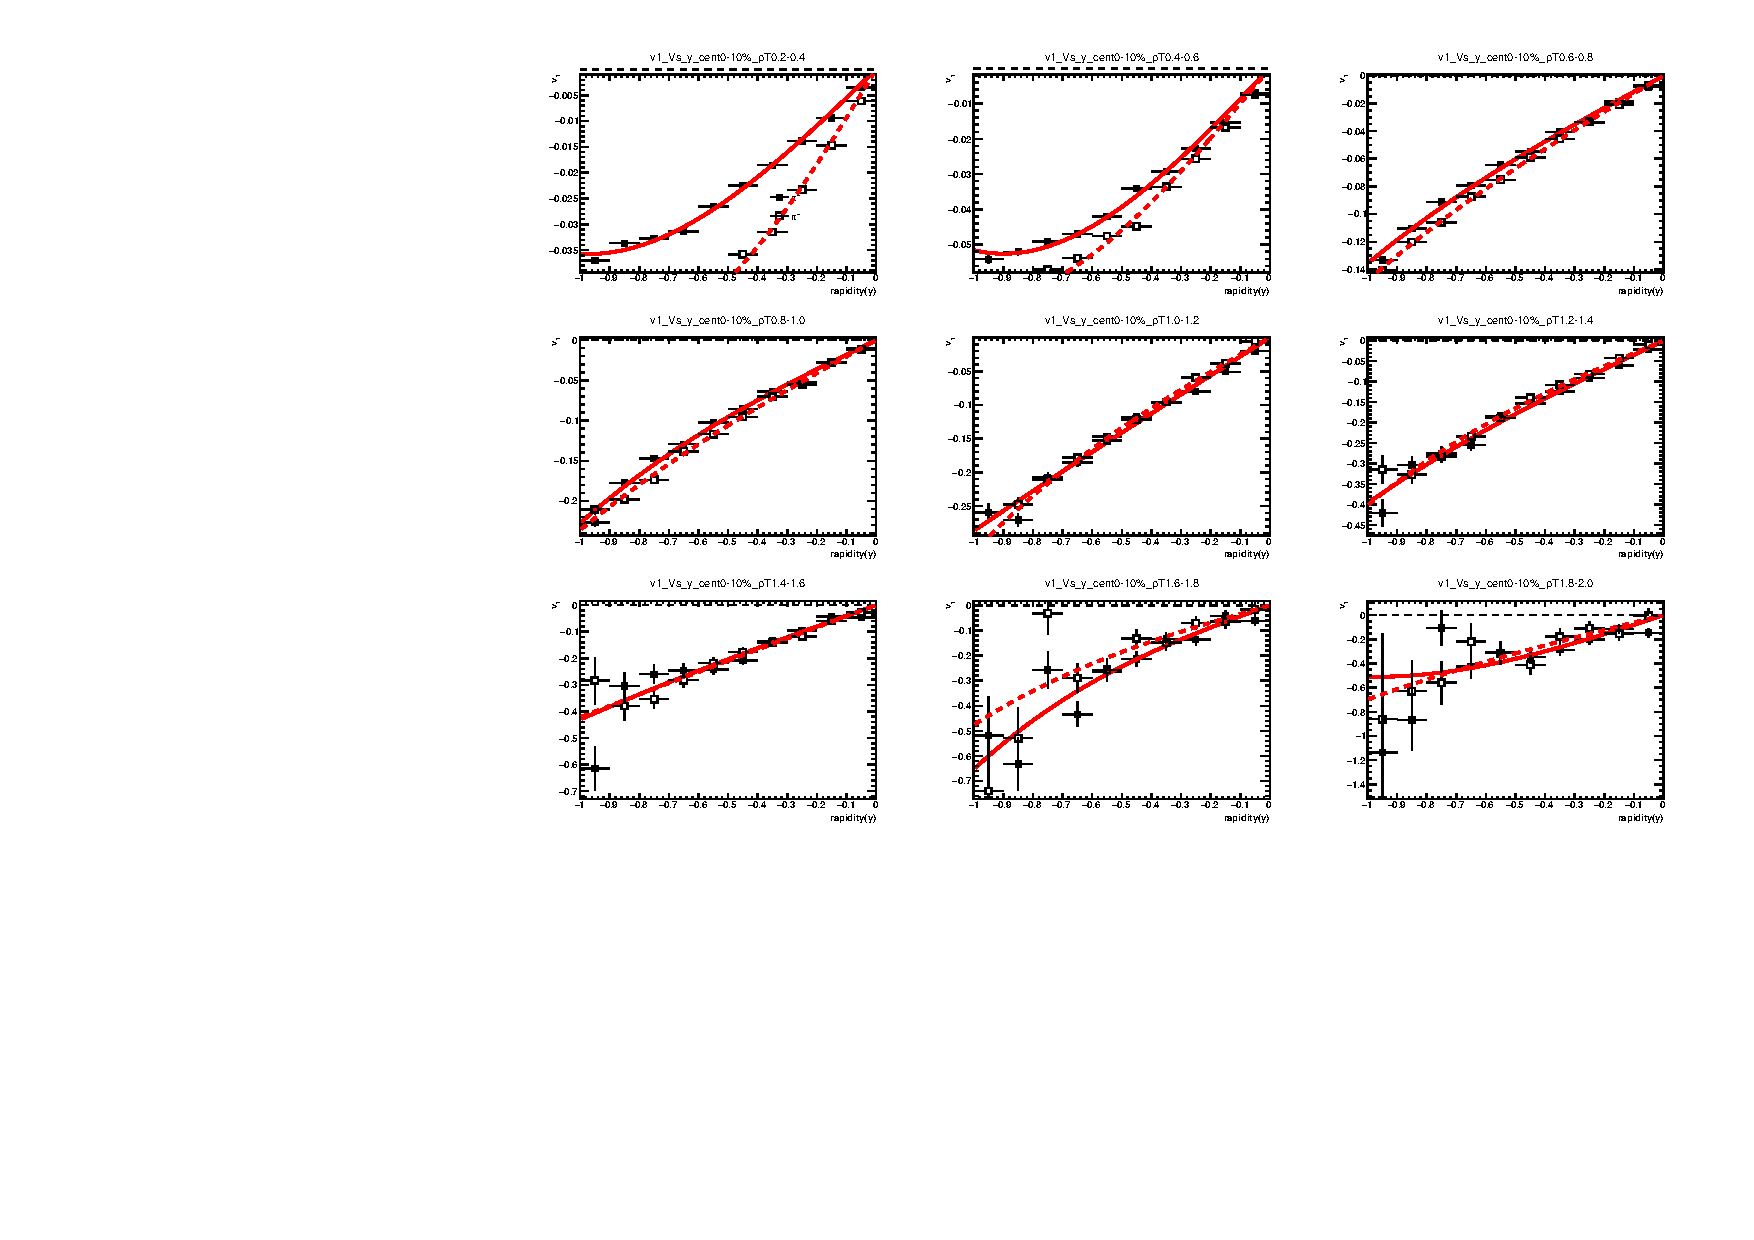
\includegraphics[width=0.85\linewidth]{figures/chapter03/3gev_pionp_v1VSy_9pT_cent2.pdf}
\caption{$v_1$ of pions as function of rapidity within $p_T$ windows in 0-10\% centrality at $\sqrt{s_{NN}}$ = 3.0 GeV.}
\label{fig:3gev_pion_v1y_pt_cent2}
\end{figure}


\begin{figure}[hbt!]
\centering
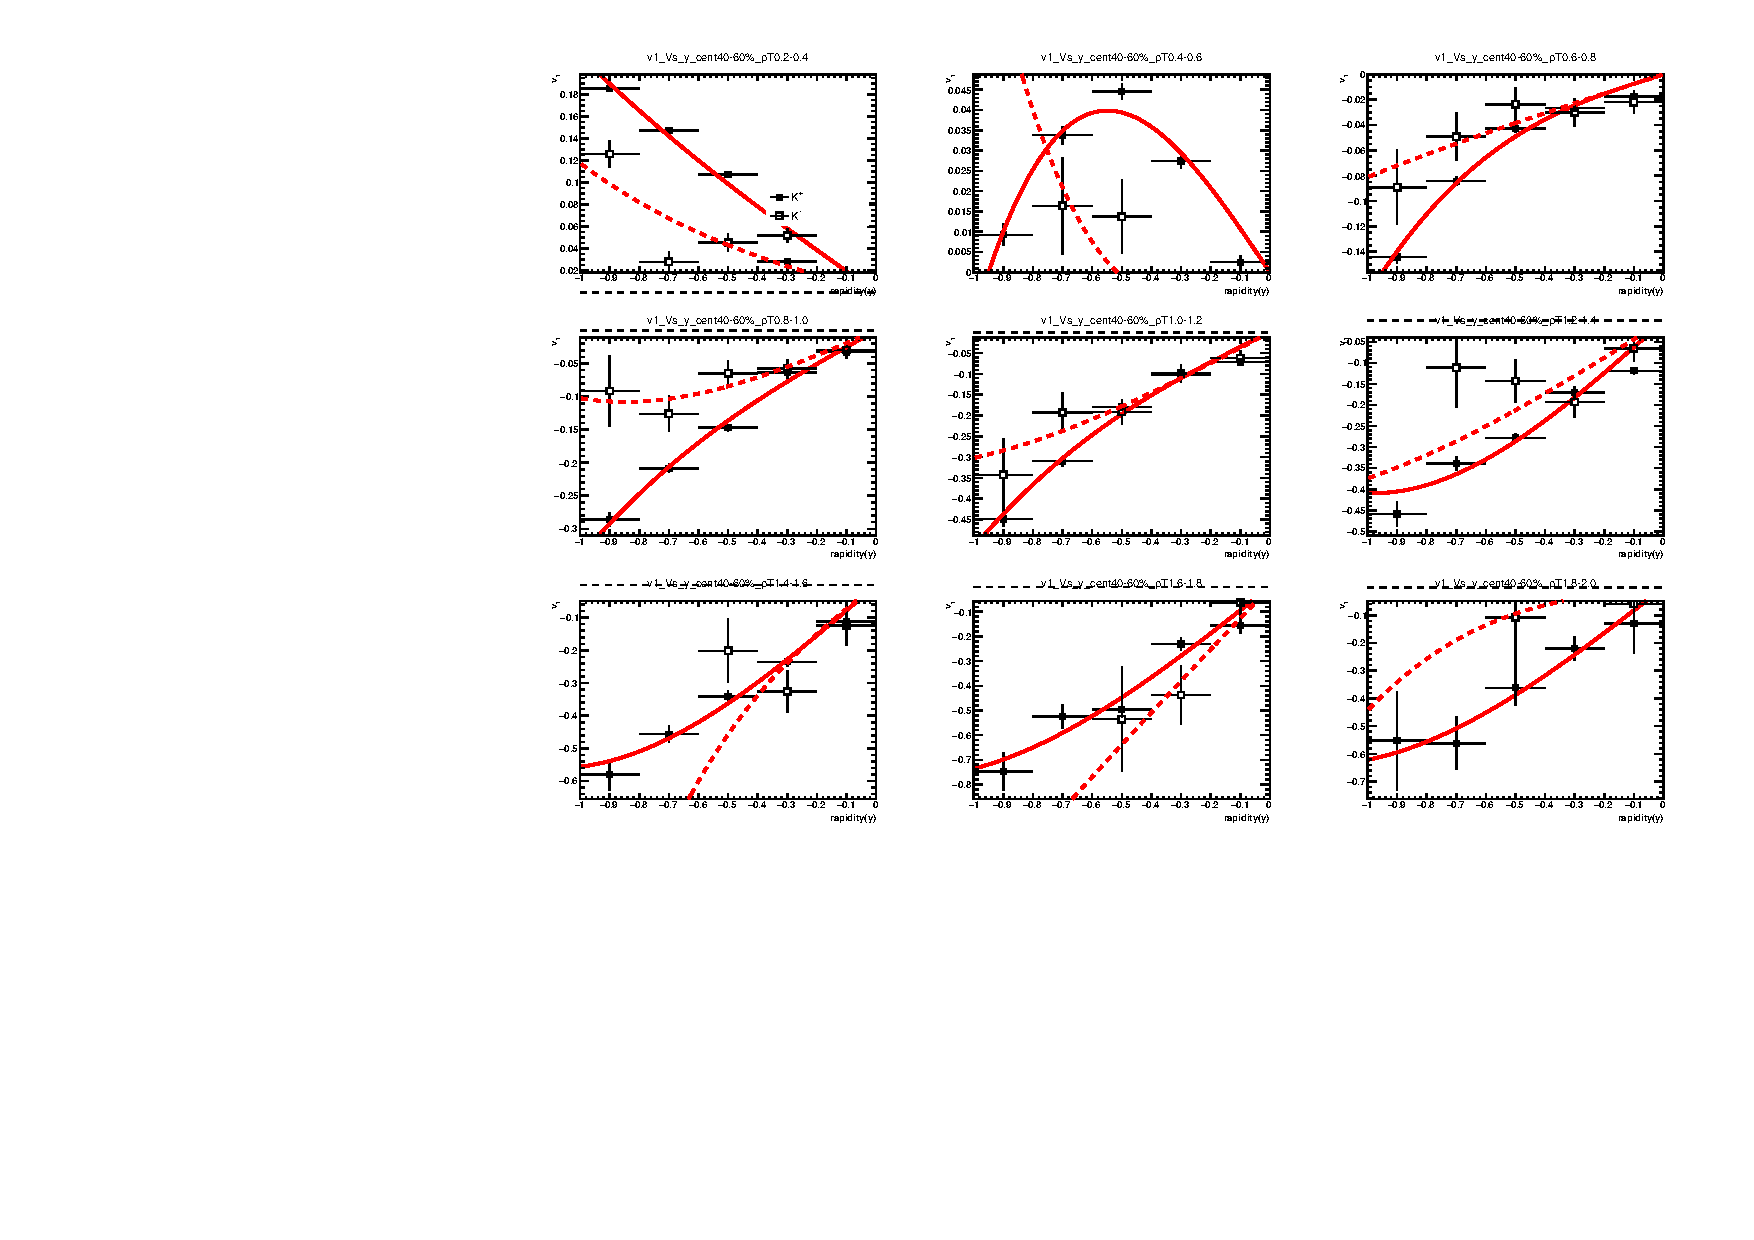
\includegraphics[width=0.85\linewidth]{figures/chapter03/3gev_kaonp_v1VSy_9pT_cent0.pdf}
\caption{$v_1$ of kaons as function of rapidity within $p_T$ windows in 40-60\% centrality at $\sqrt{s_{NN}}$ = 3.0 GeV.}
\label{fig:3gev_kaon_v1y_pt_cent0}
\end{figure}
        
\begin{figure}[hbt!]
\centering
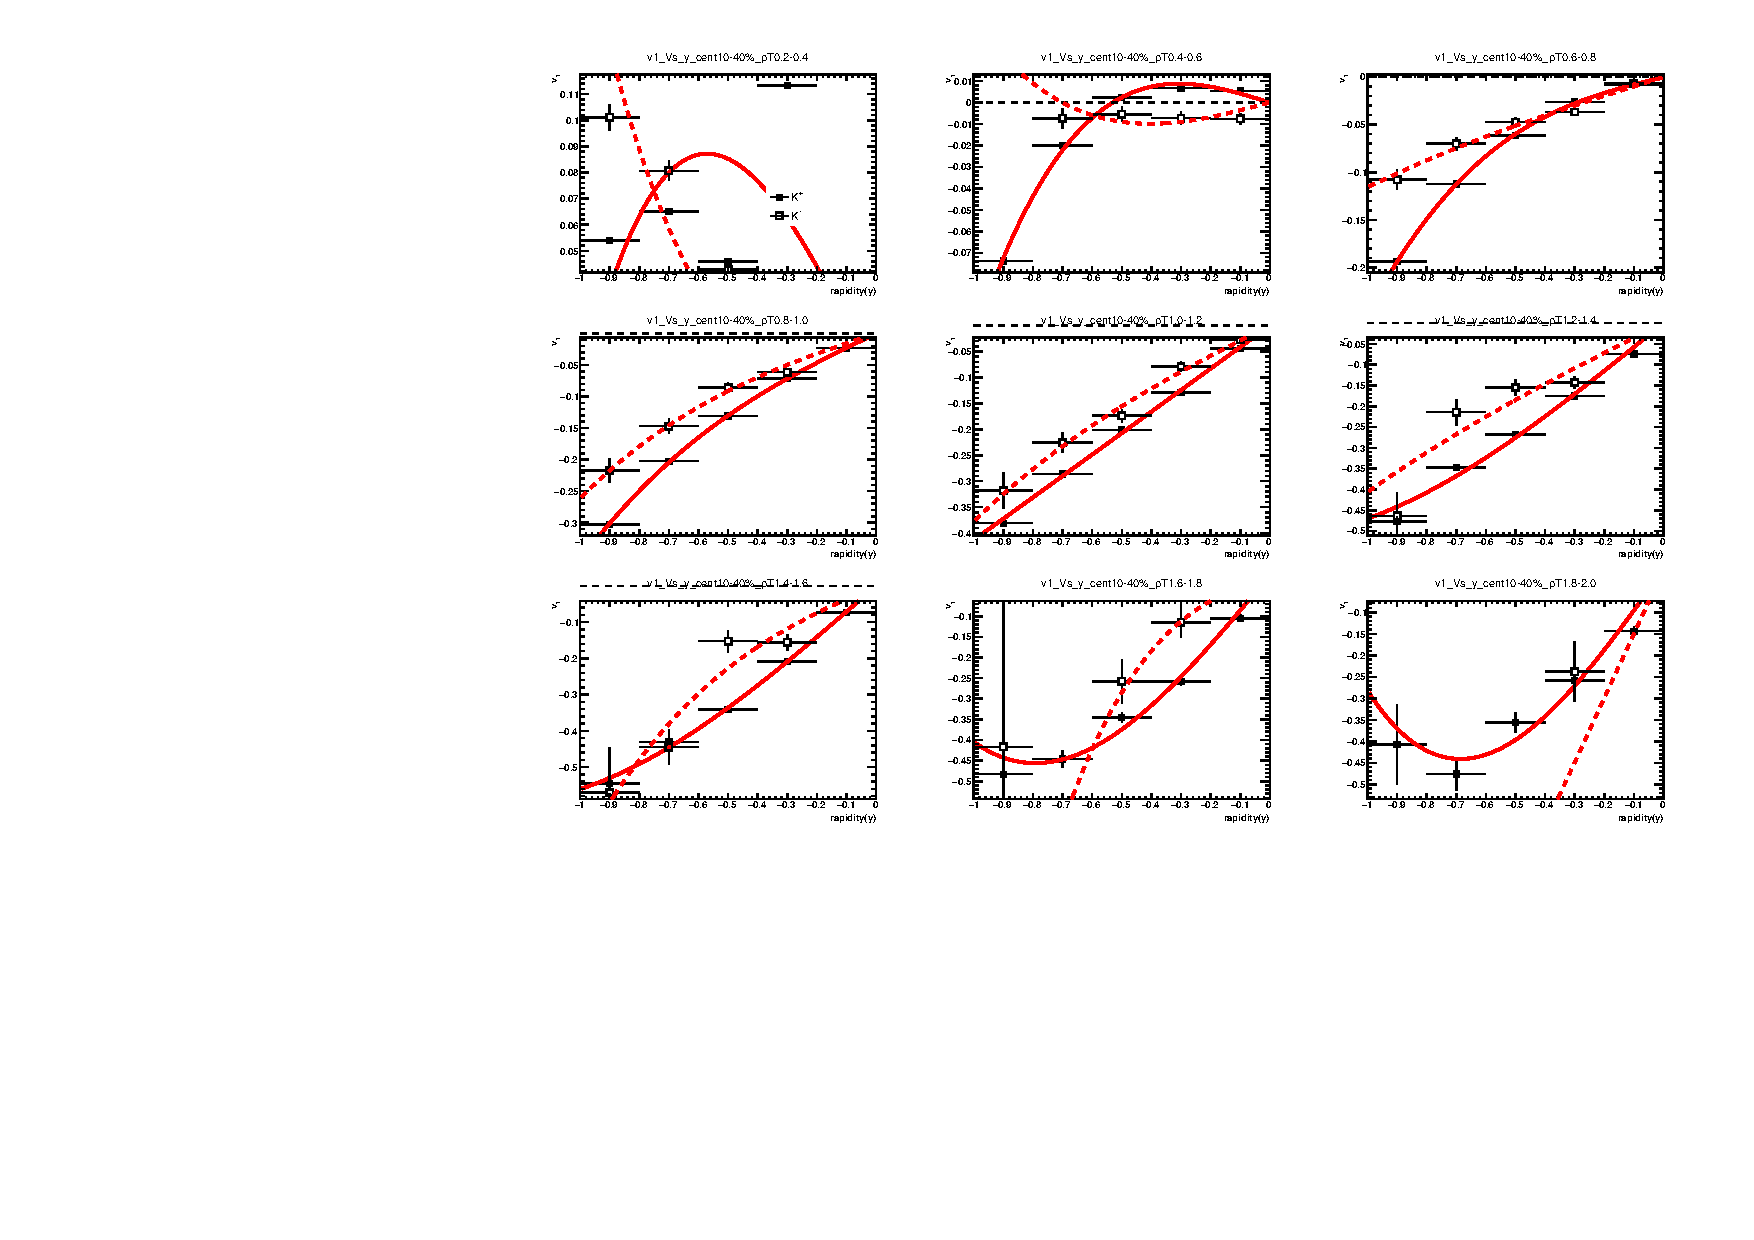
\includegraphics[width=0.85\linewidth]{figures/chapter03/3gev_kaonp_v1VSy_9pT_cent1.pdf}
\caption{$v_1$ of kaons as function of rapidity within $p_T$ windows in 10-40\% centrality at $\sqrt{s_{NN}}$ = 3.0 GeV.}
\label{fig:3gev_kaon_v1y_pt_cent1}
\end{figure}
            
\begin{figure}[hbt!]
\centering
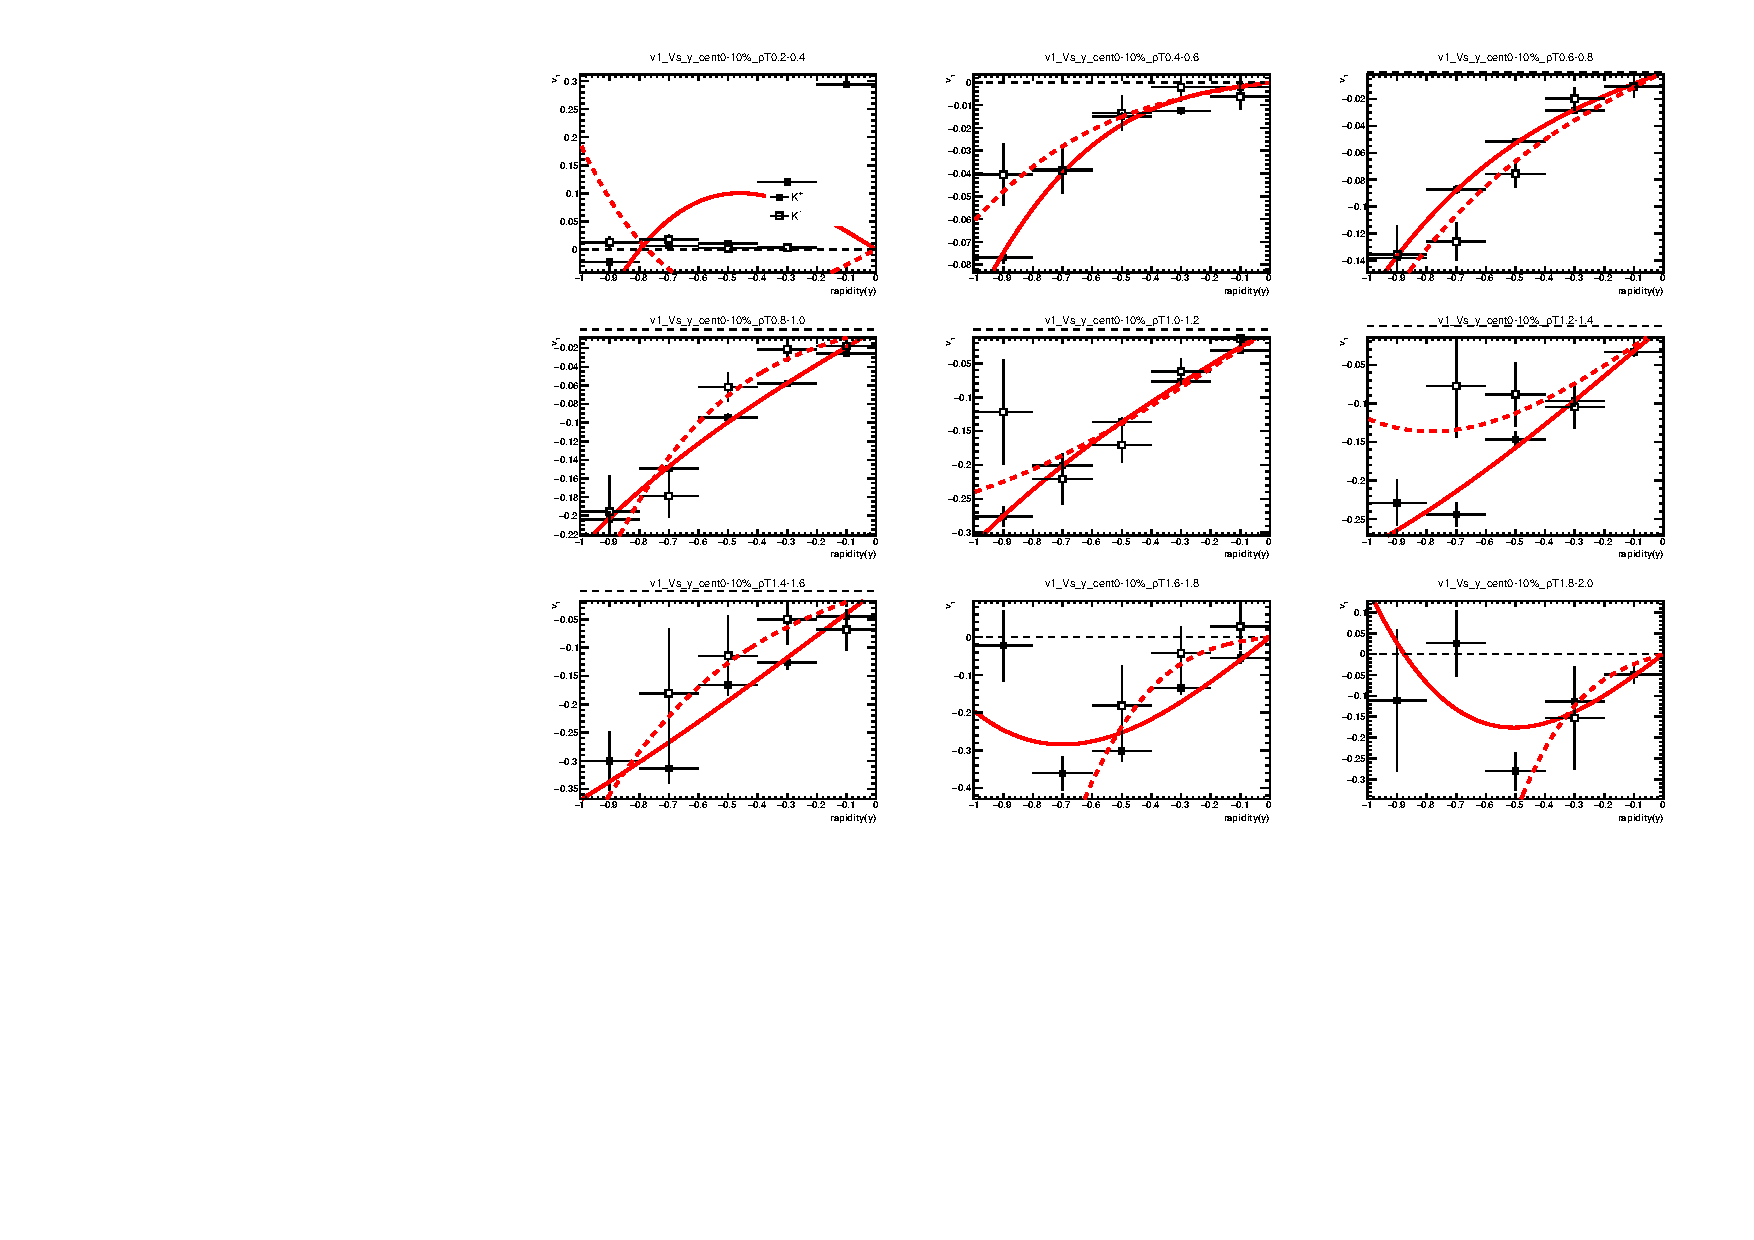
\includegraphics[width=0.85\linewidth]{figures/chapter03/3gev_kaonp_v1VSy_9pT_cent2.pdf}
\caption{$v_1$ of kaons as function of rapidity within $p_T$ windows in 0-10\% centrality at $\sqrt{s_{NN}}$ = 3.0 GeV.}
\label{fig:3gev_kaon_v1y_pt_cent2}
\end{figure}


\begin{figure}[hbt!]
\centering
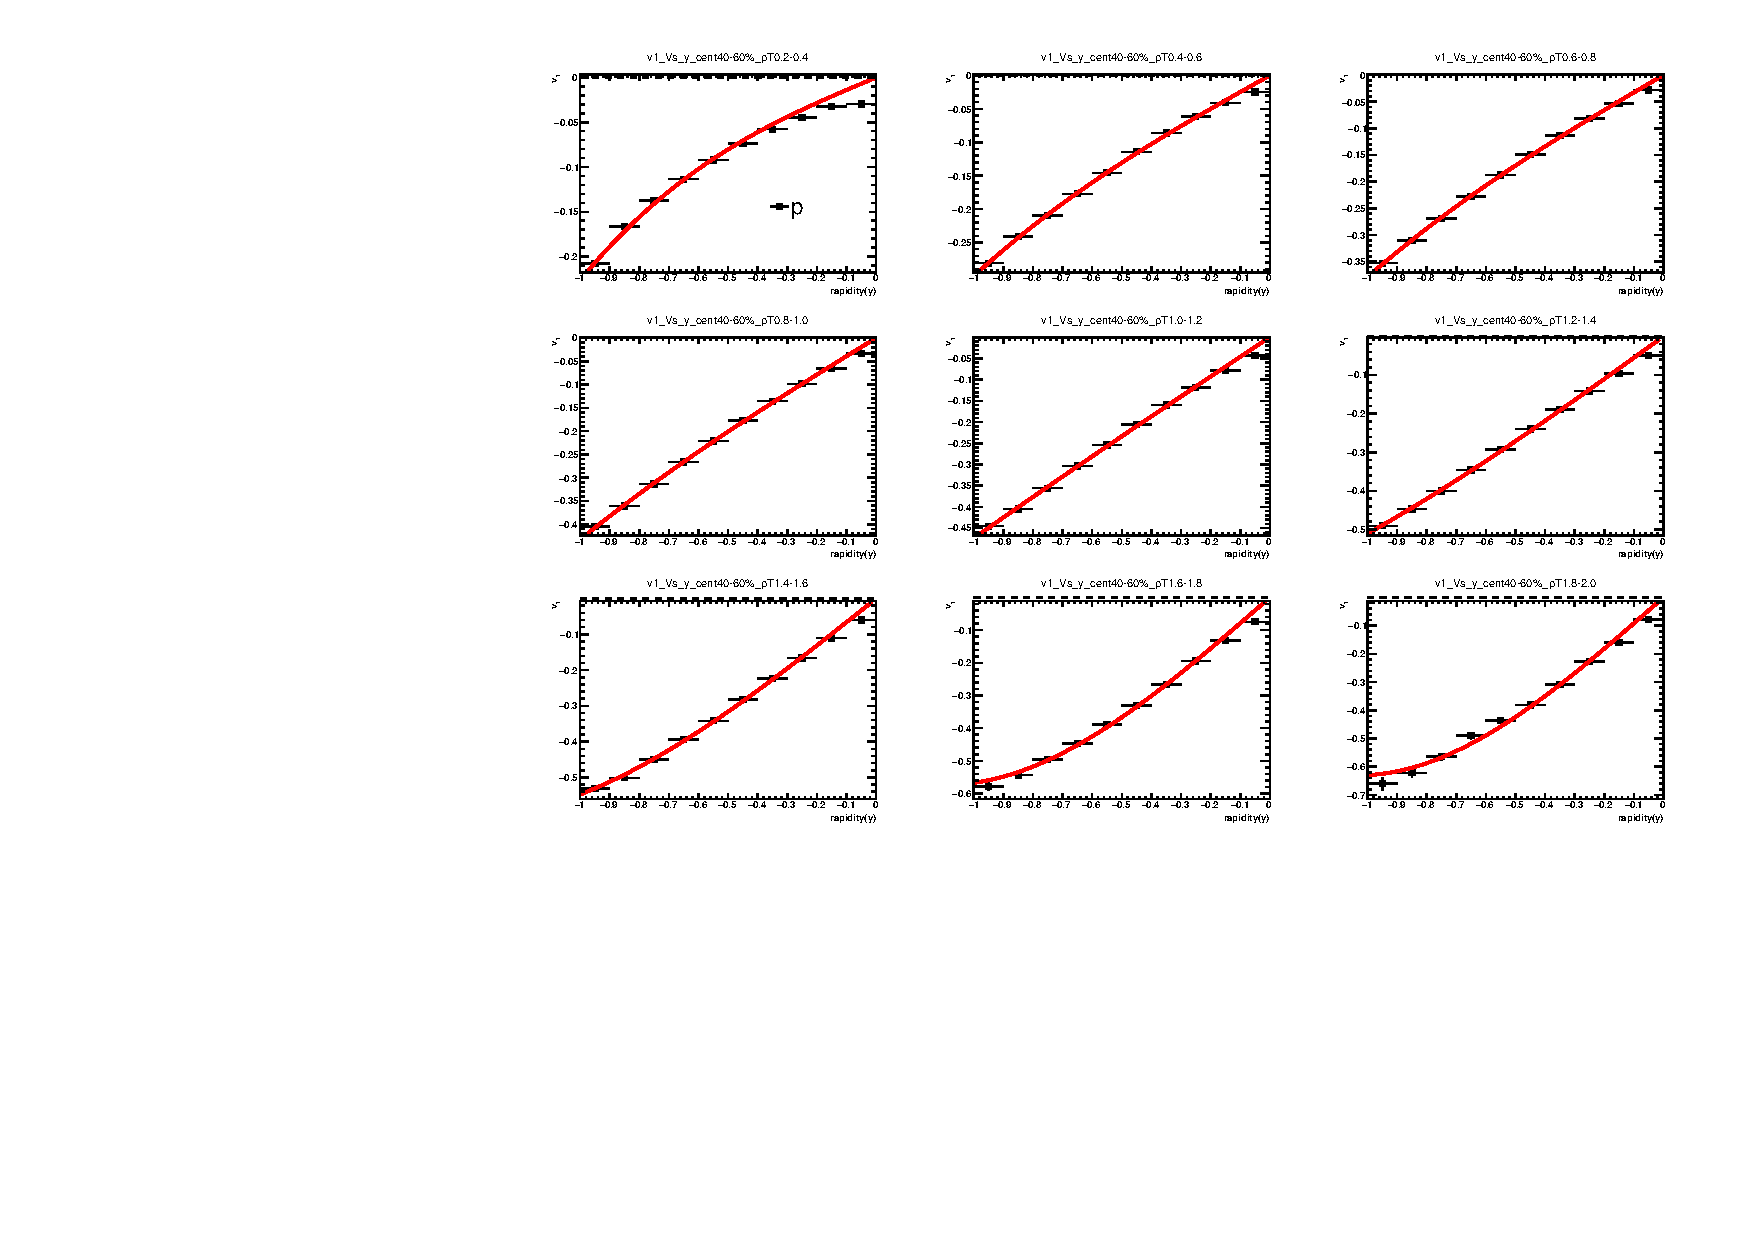
\includegraphics[width=0.85\linewidth]{figures/chapter03/3gev_protonp_v1VSy_9pT_cent0.pdf}
\caption{$v_1$ of protons as function of rapidity within $p_T$ windows in 40-60\% centrality at $\sqrt{s_{NN}}$ = 3.0 GeV.}
\label{fig:3gev_proton_v1y_pt_cent0}
\end{figure}
            
\begin{figure}[hbt!]
\centering
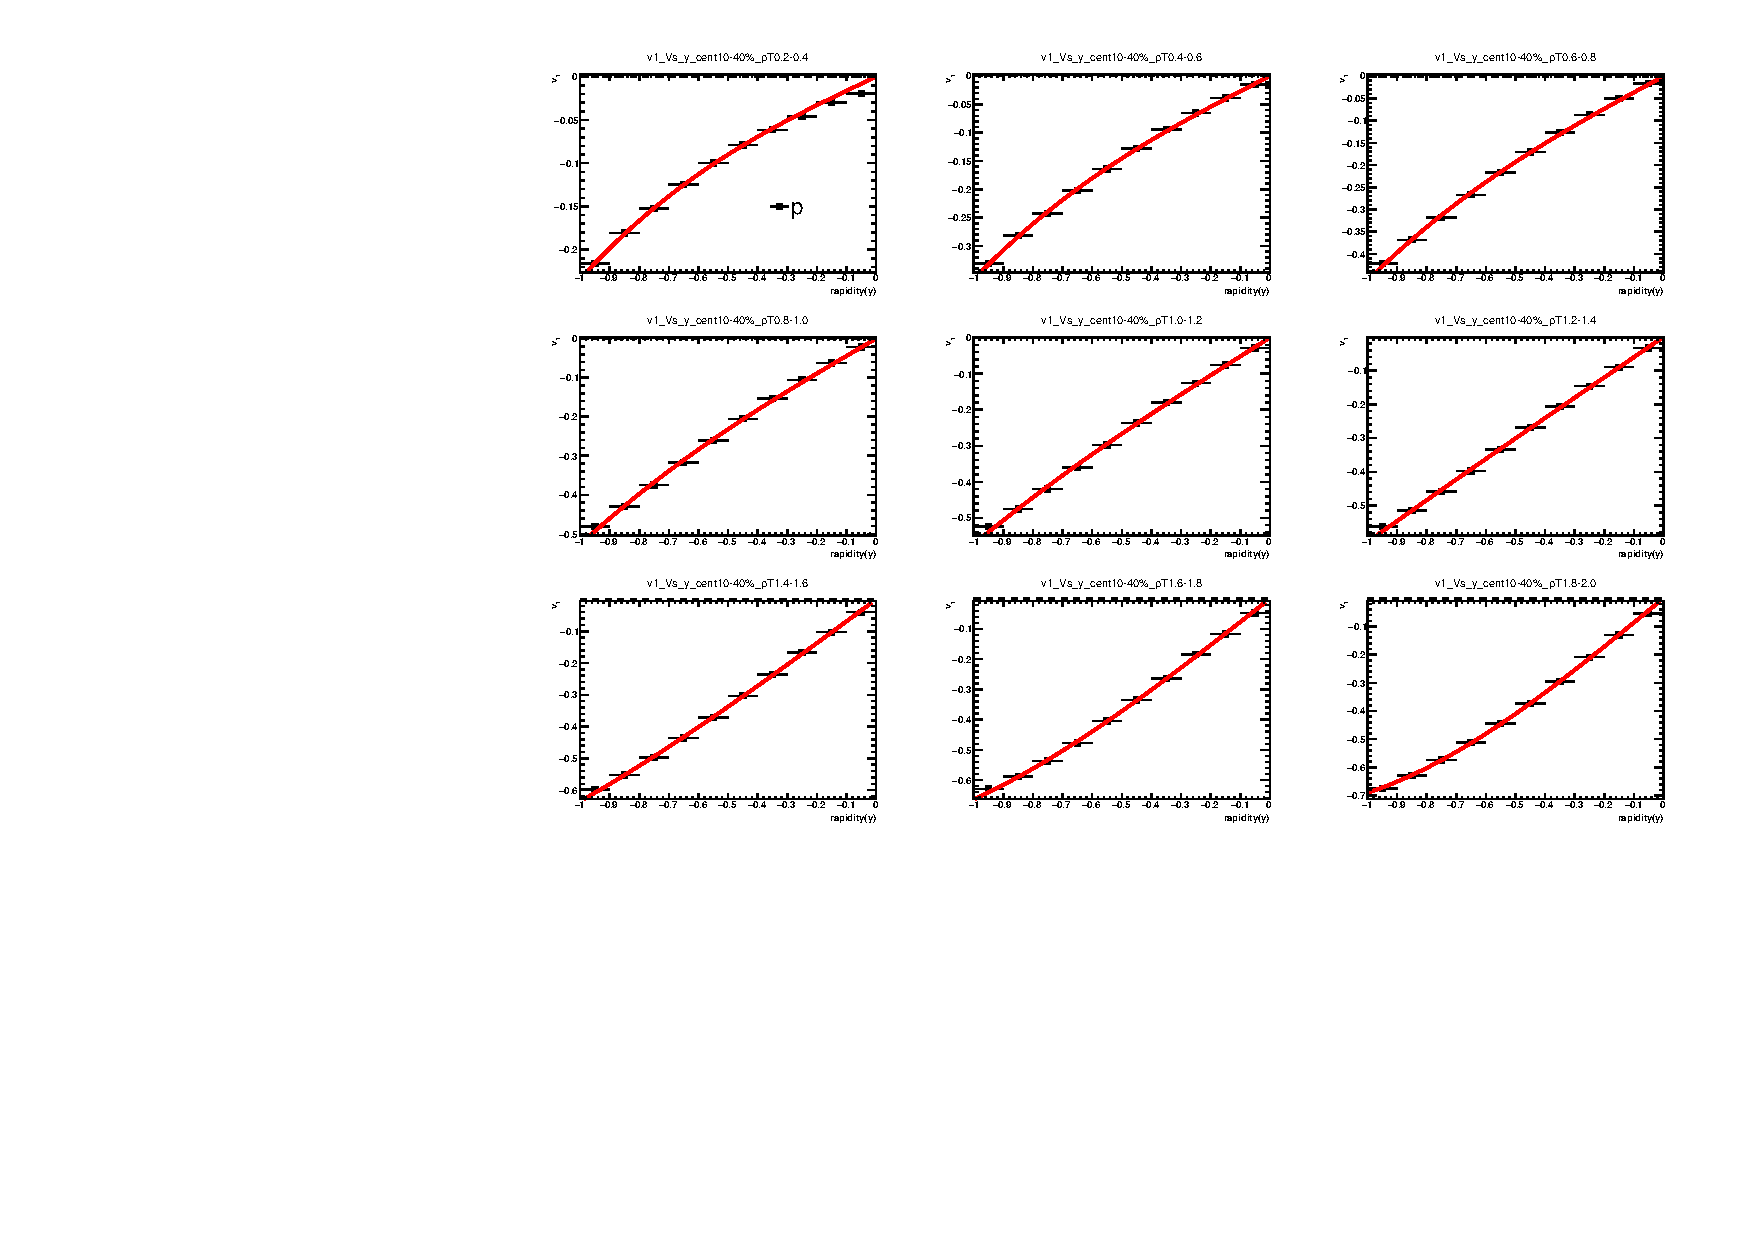
\includegraphics[width=0.85\linewidth]{figures/chapter03/3gev_protonp_v1VSy_9pT_cent1.pdf}
\caption{$v_1$ of protons as function of rapidity within $p_T$ windows in 10-40\% centrality at $\sqrt{s_{NN}}$ = 3.0 GeV.}
\label{fig:3gev_proton_v1y_pt_cent1}
\end{figure}
                
\begin{figure}[hbt!]
\centering
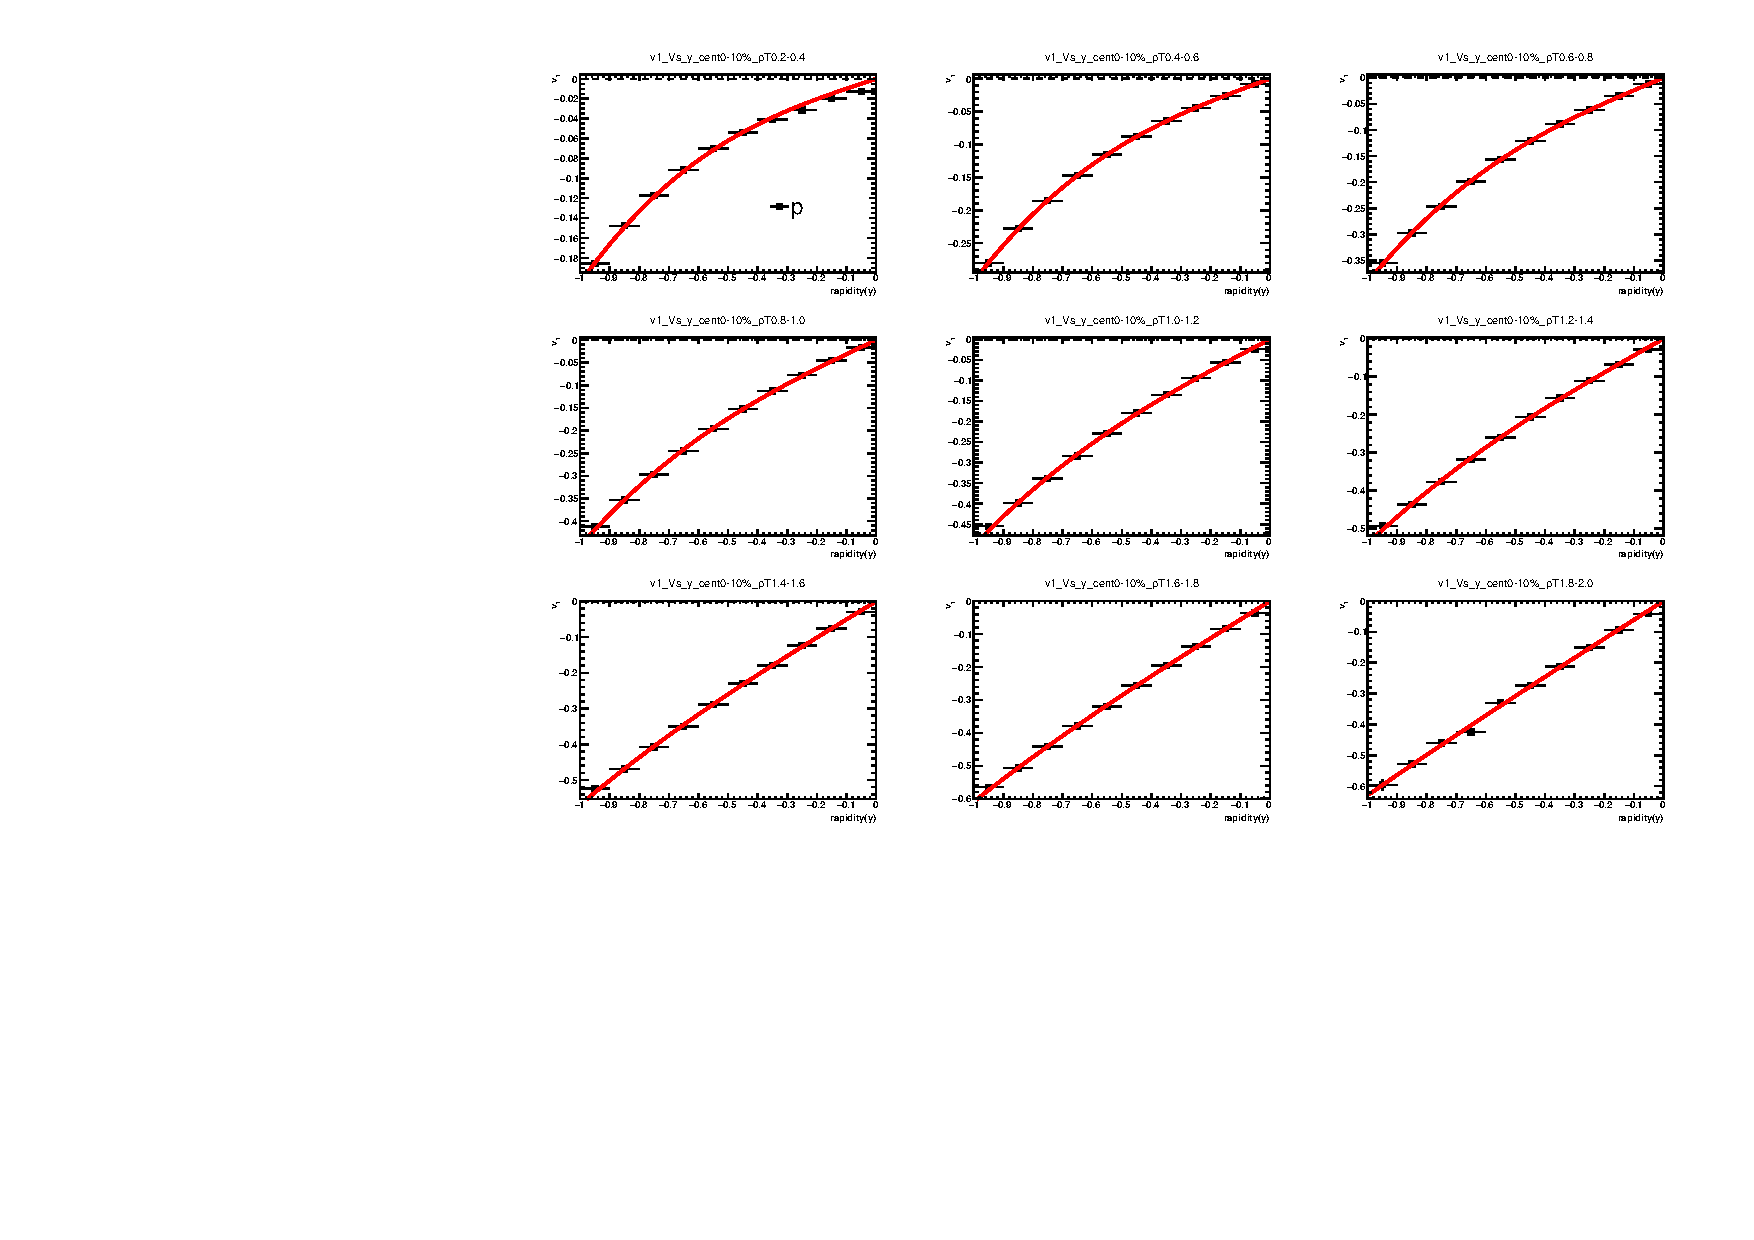
\includegraphics[width=0.85\linewidth]{figures/chapter03/3gev_protonp_v1VSy_9pT_cent2.pdf}
\caption{$v_1$ of protons as function of rapidity within $p_T$ windows in 0-10\% centrality at $\sqrt{s_{NN}}$ = 3.0 GeV.}
\label{fig:3gev_proton_v1y_pt_cent2}
\end{figure}


\begin{figure}[hbt!]
\centering
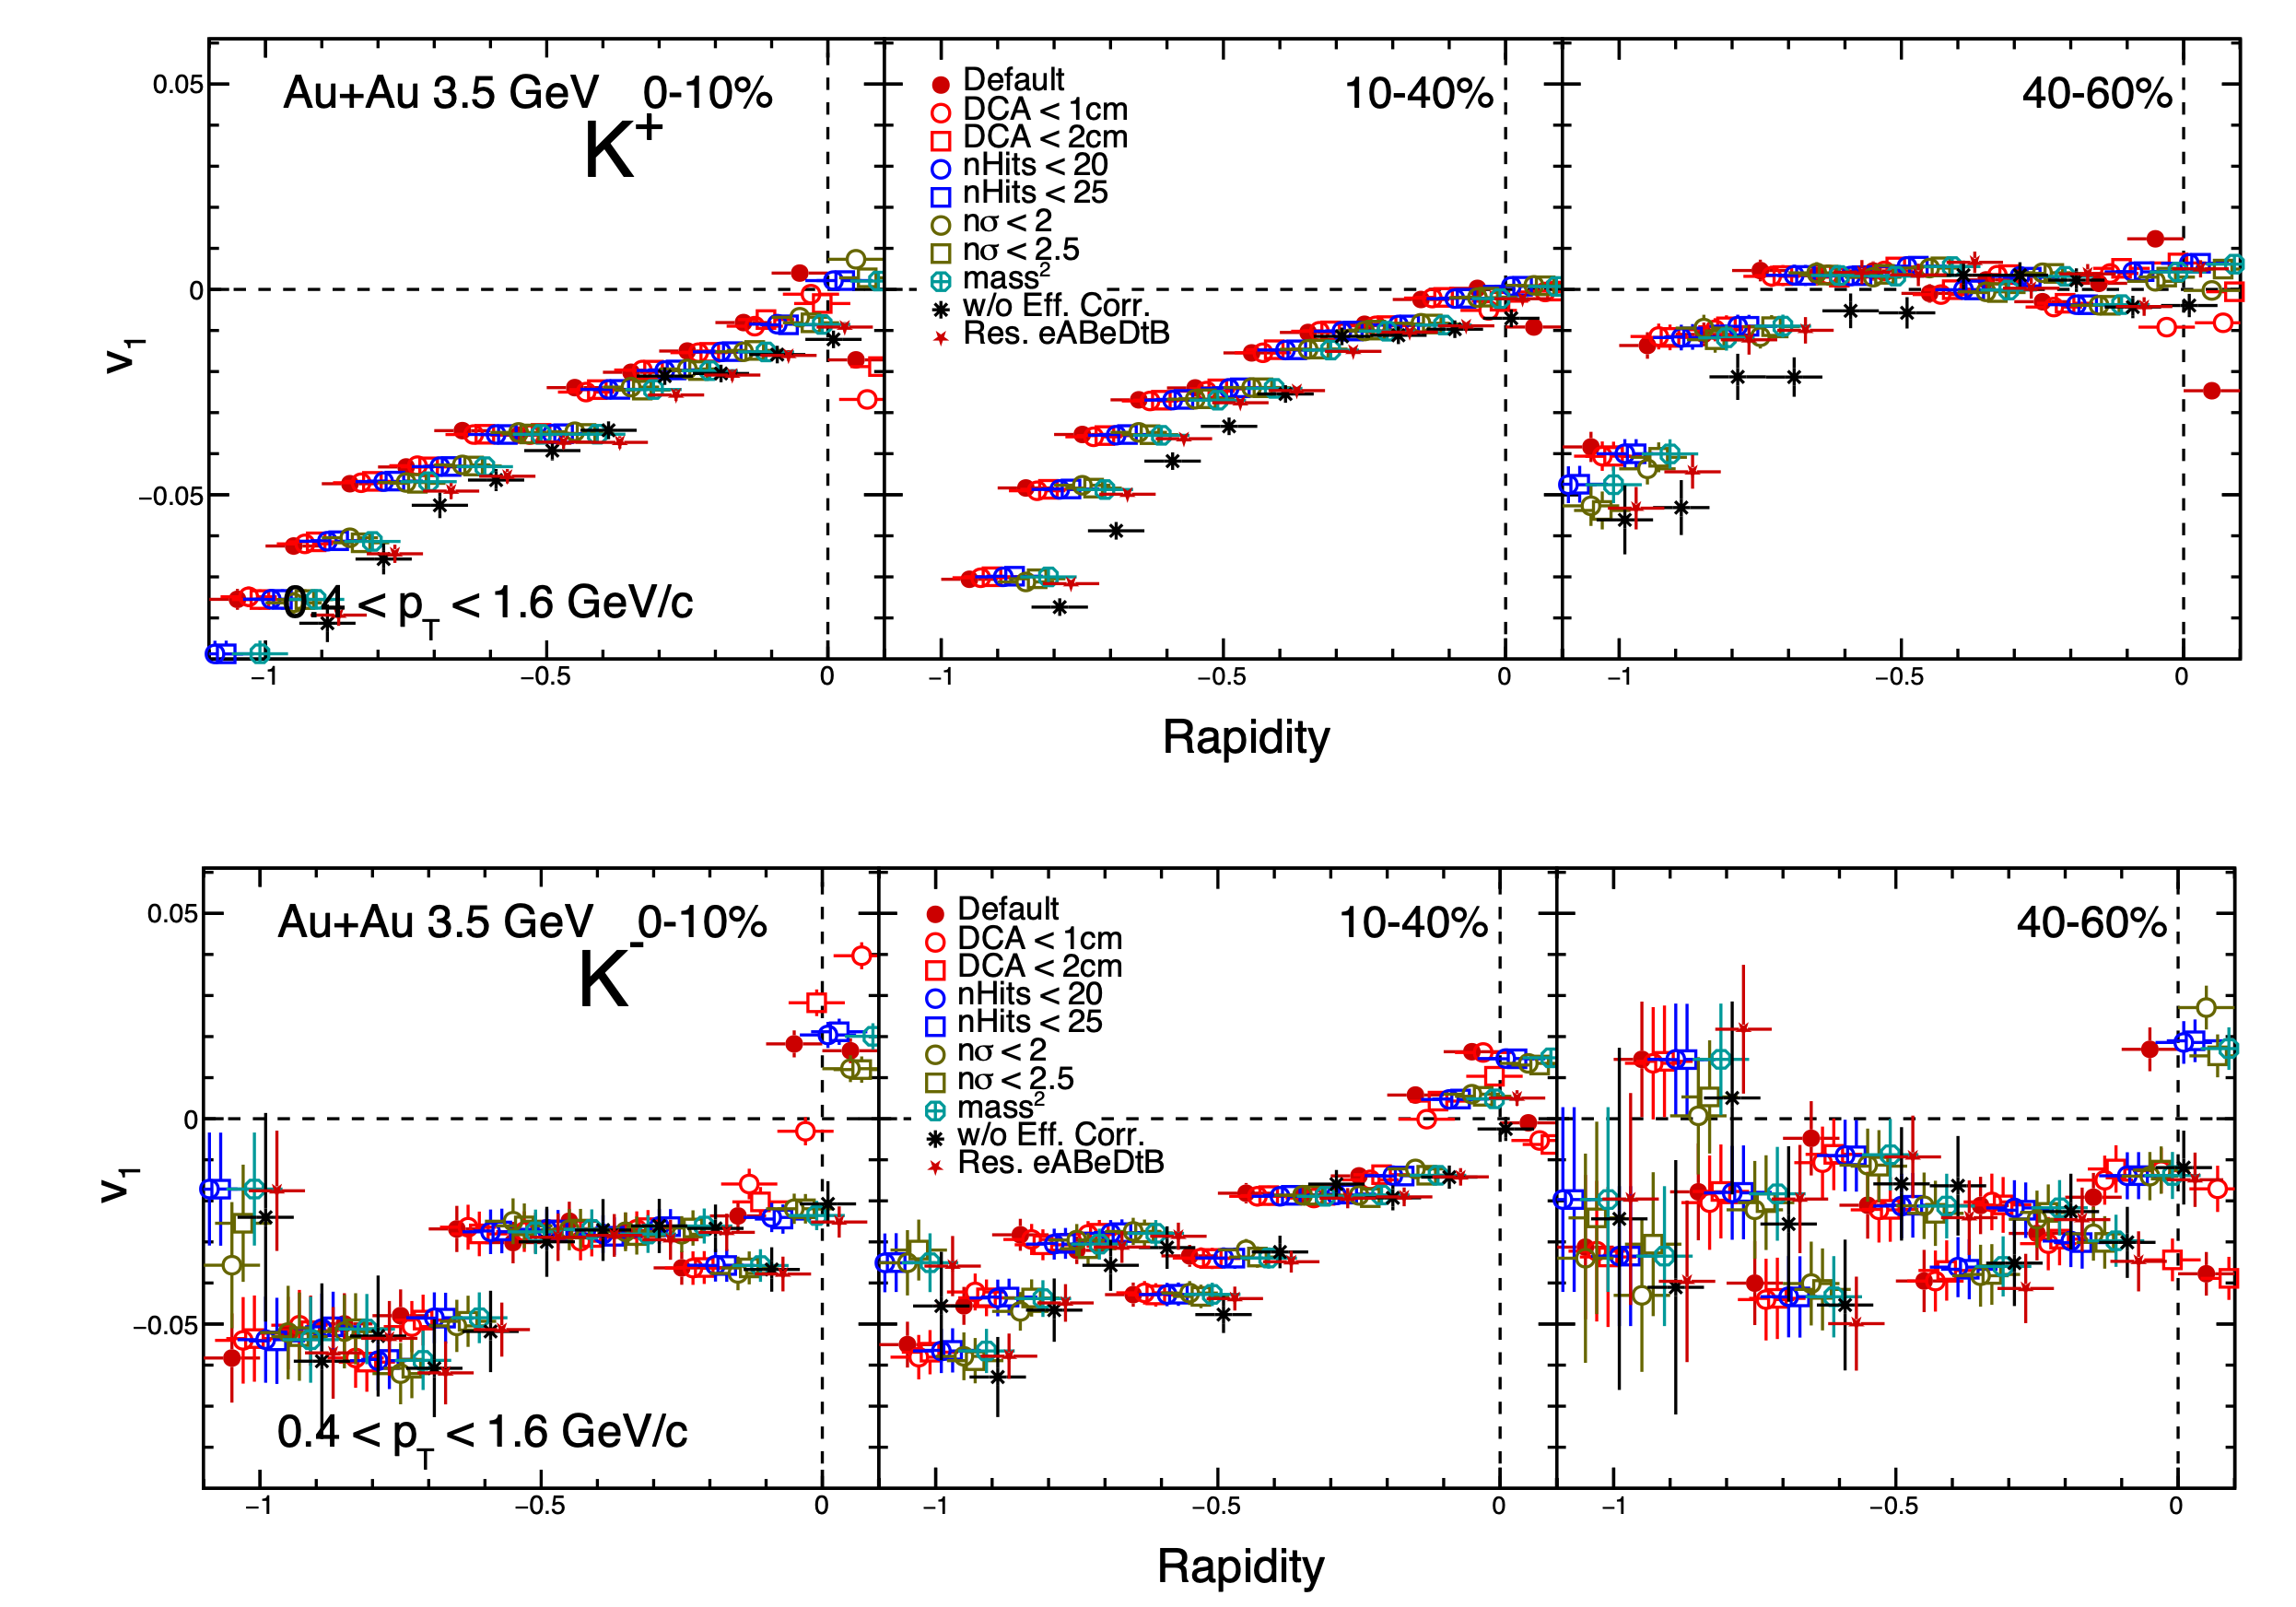
\includegraphics[width=0.95\linewidth]{figures/chapter03/3p5gev_kaon_v1y_sysUnc.png}
\caption{$v_1$ of kaons as function of rapidity from systematic sources at $\sqrt{s_{NN}}$ = 3.5 GeV.}
\label{fig:3p5gev_kaon_v1y_sysUnc}
\end{figure}

\begin{figure}[hbt!]
\centering
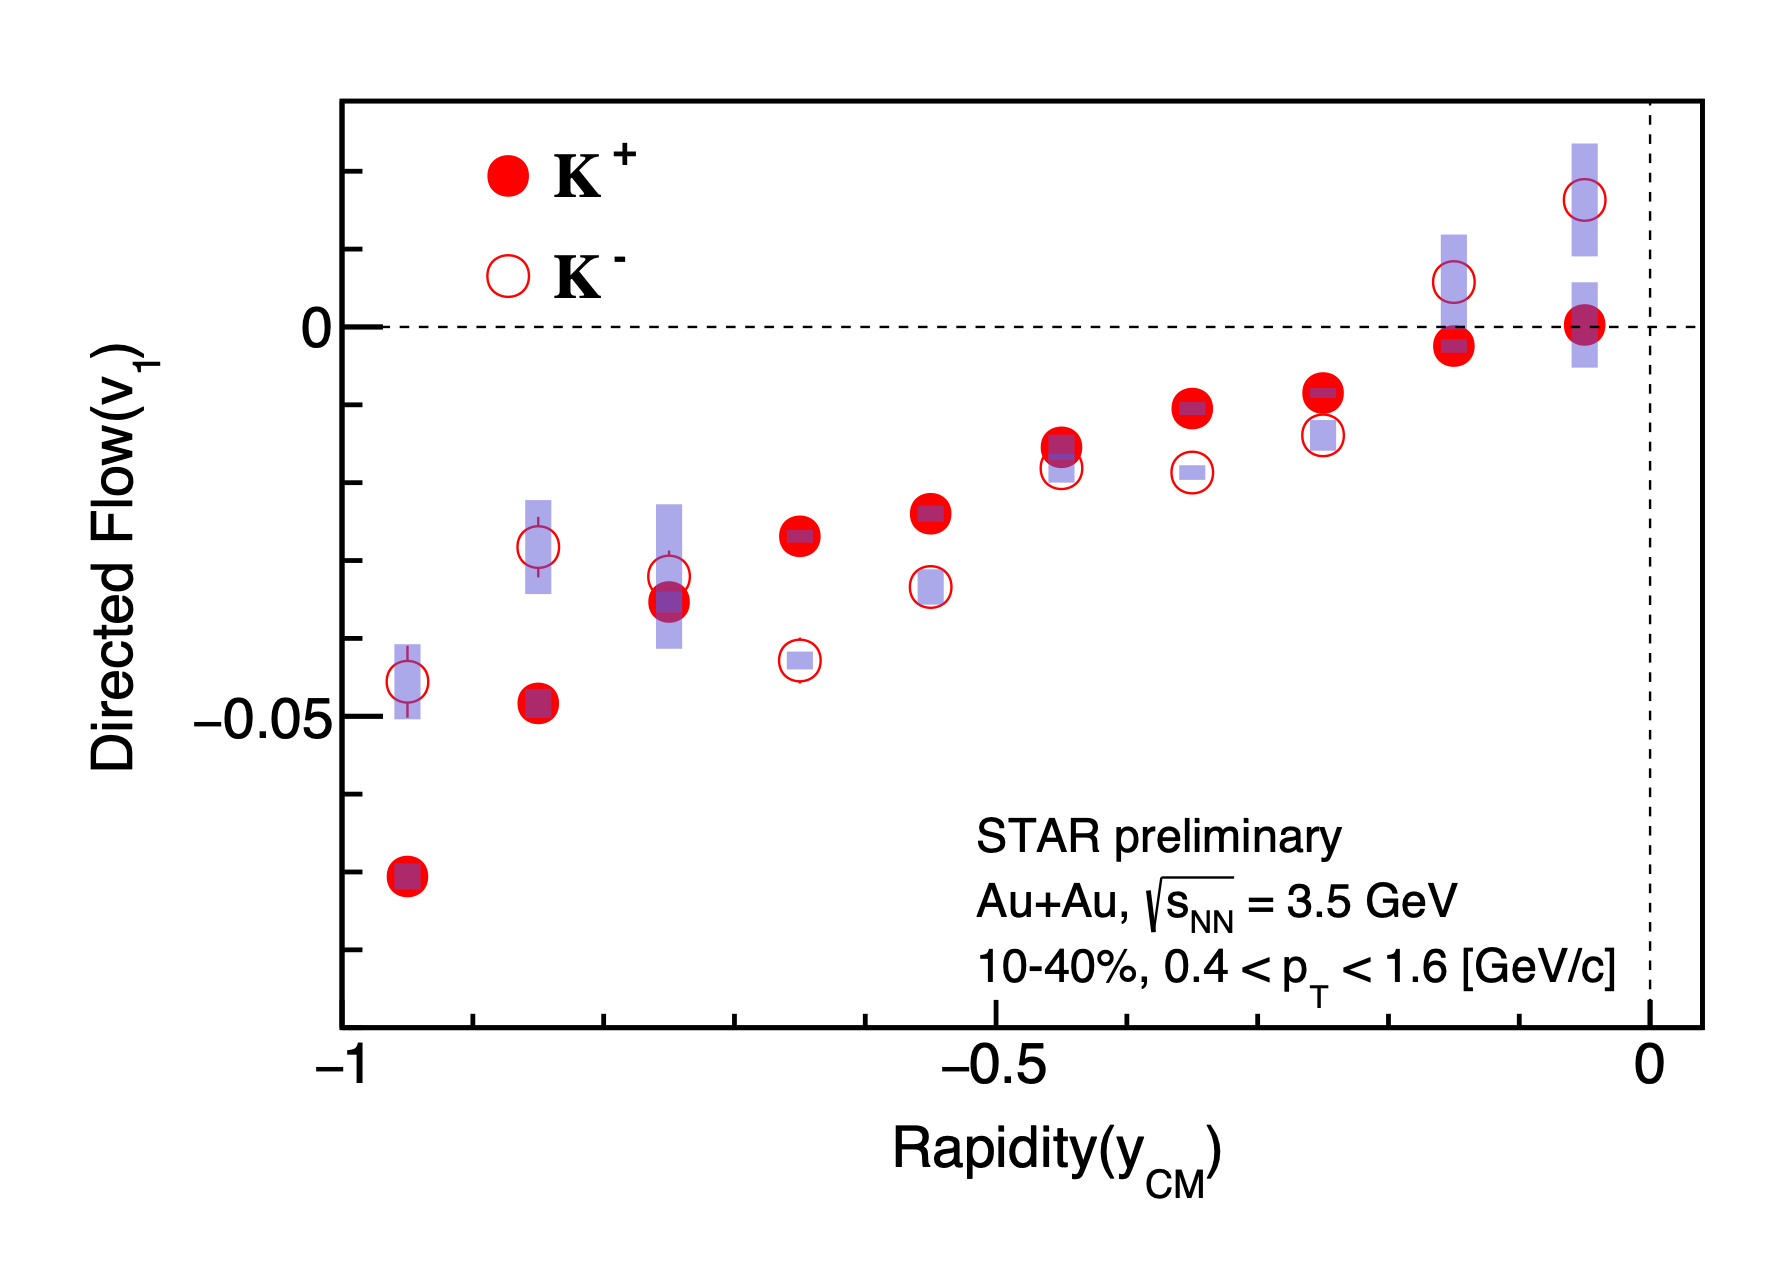
\includegraphics[width=0.65\linewidth]{figures/chapter03/3p5gev_kaon_v1y.png}
\caption{$v_1$ of kaons as function of rapidity at $\sqrt{s_{NN}}$ = 3.5 GeV.}
\label{fig:3p5gev_kaon_v1y}
\end{figure}

\begin{figure}[hbt!]
\centering
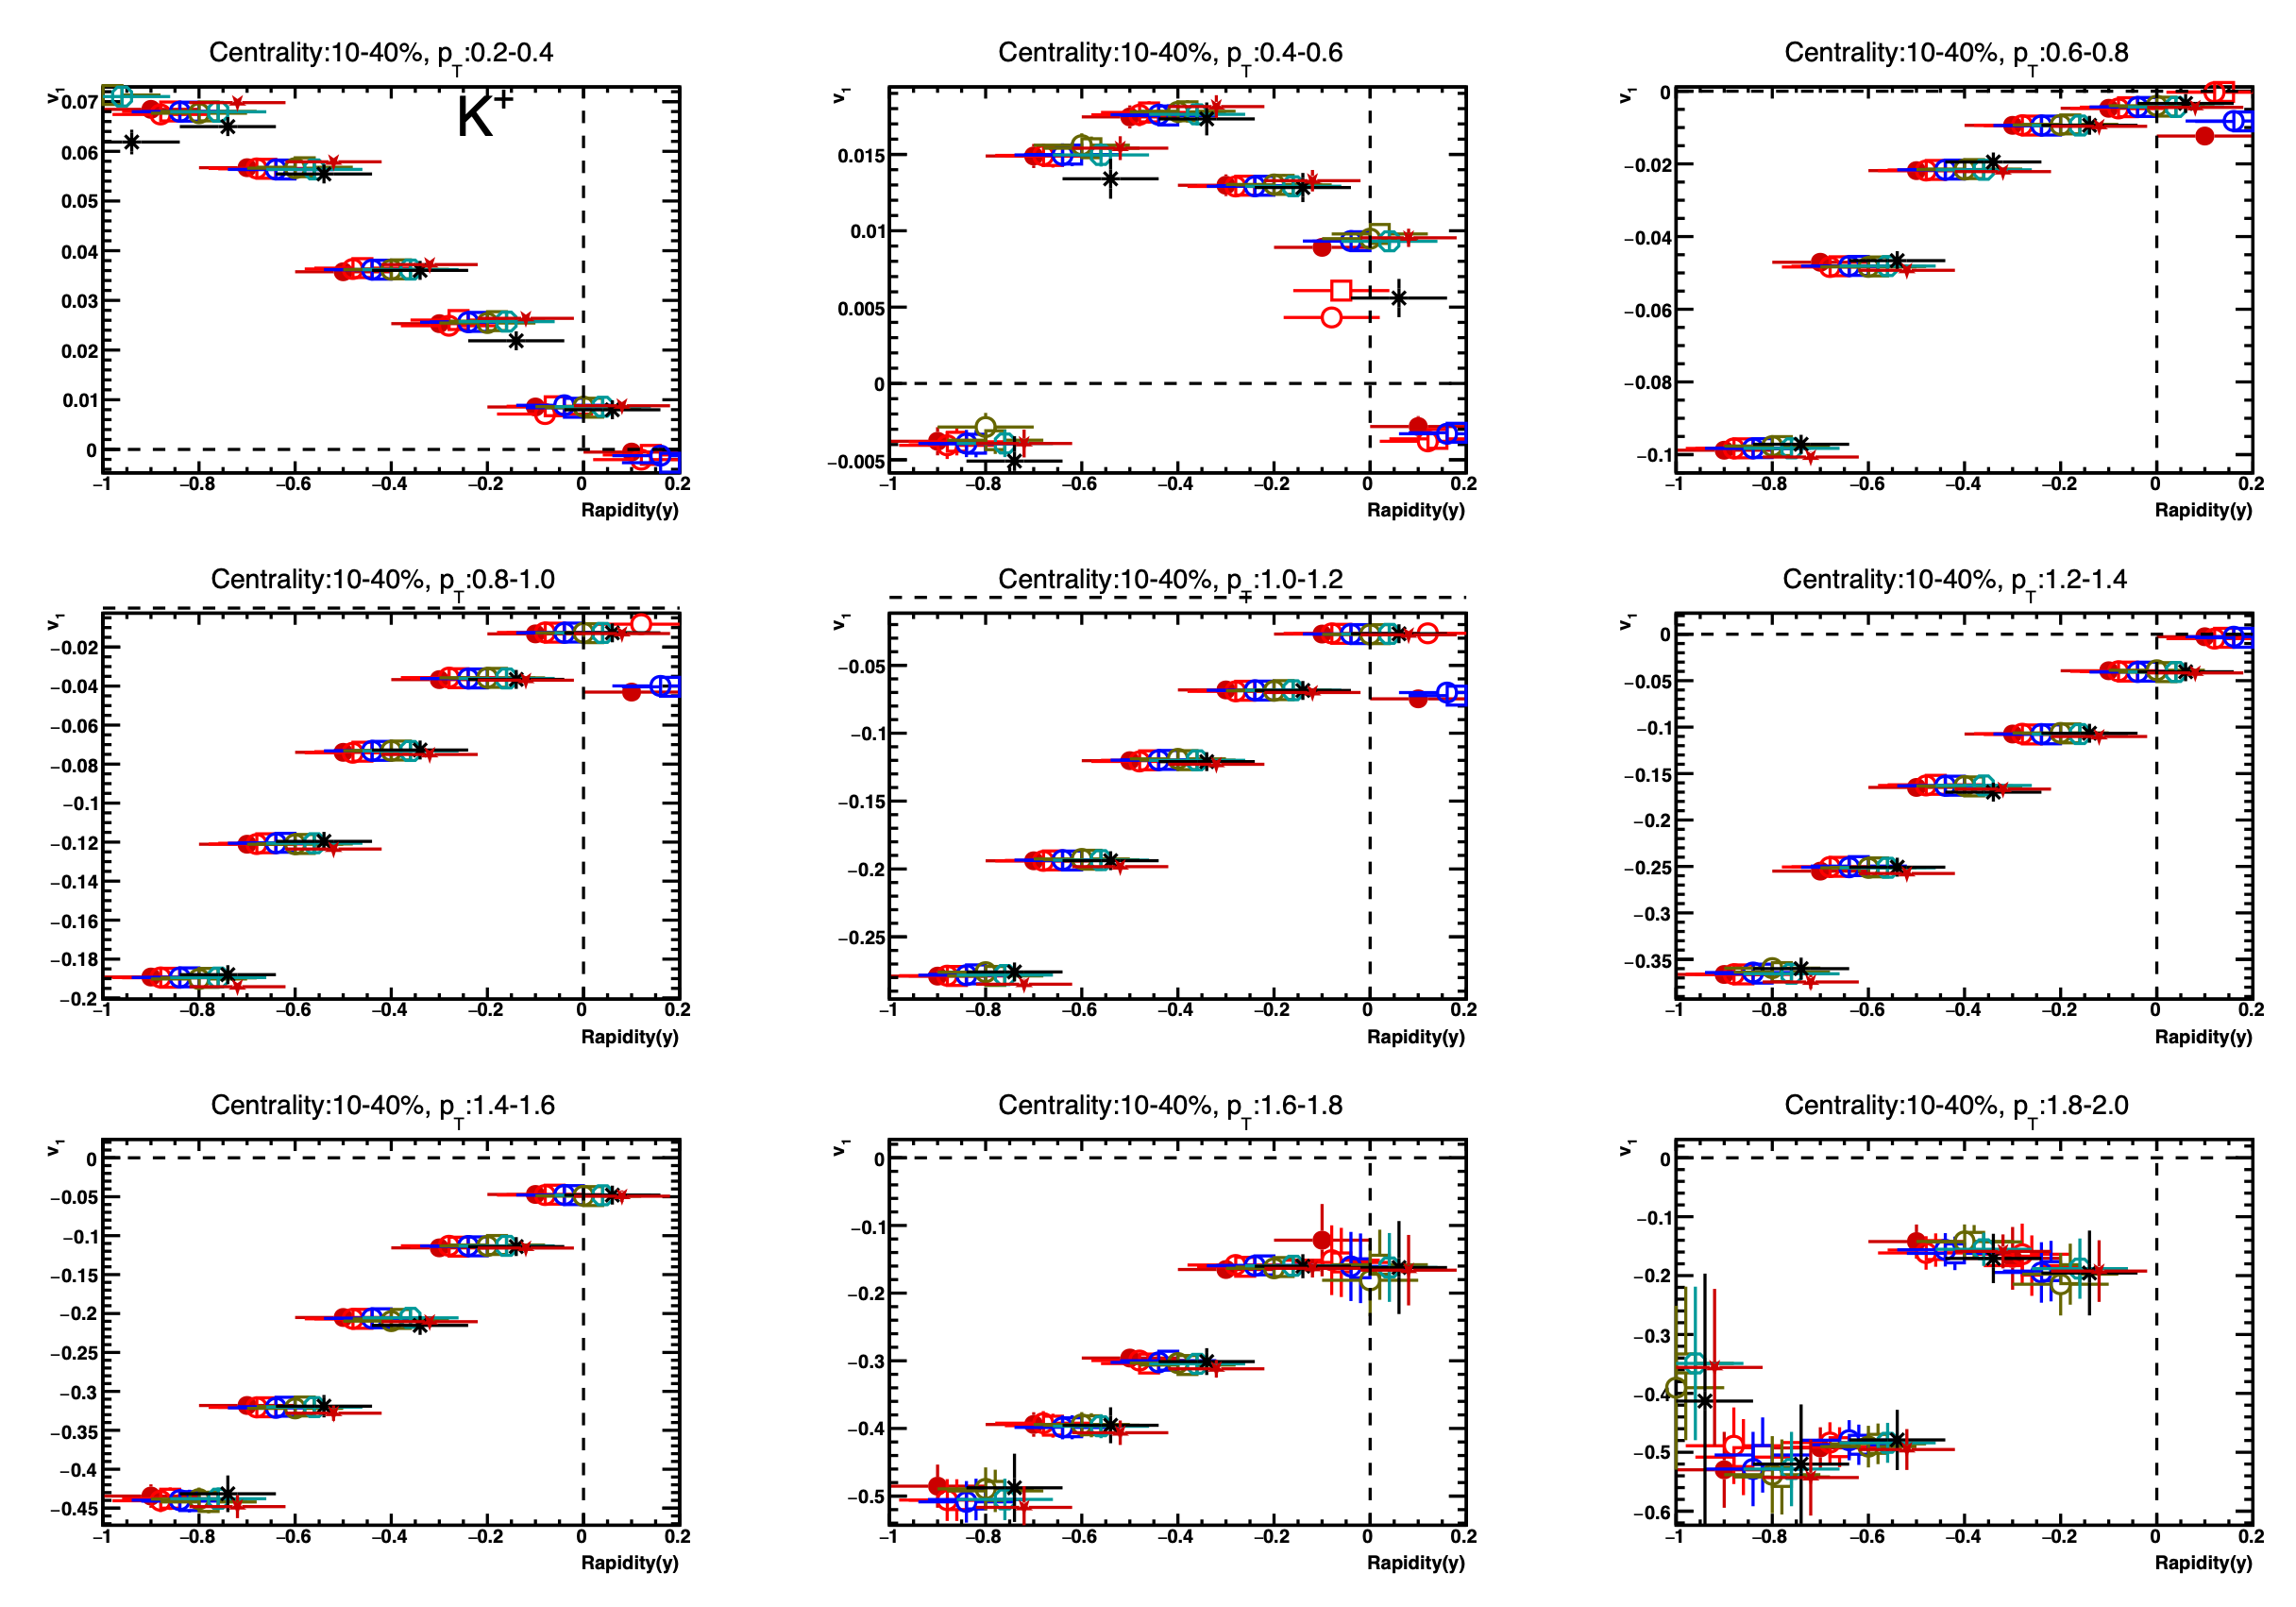
\includegraphics[width=0.95\linewidth]{figures/chapter03/3p5gev_kaonplus_v1yPt_sysUnc.png}
\caption{$v_1$ of $K^+$ as function of rapidity within $p_T$ windows at $\sqrt{s_{NN}}$ = 3.5 GeV.}
\label{fig:3p5gev_kaonplus_v1yPt_sysUnc}
\end{figure}

\begin{figure}[hbt!]
\centering
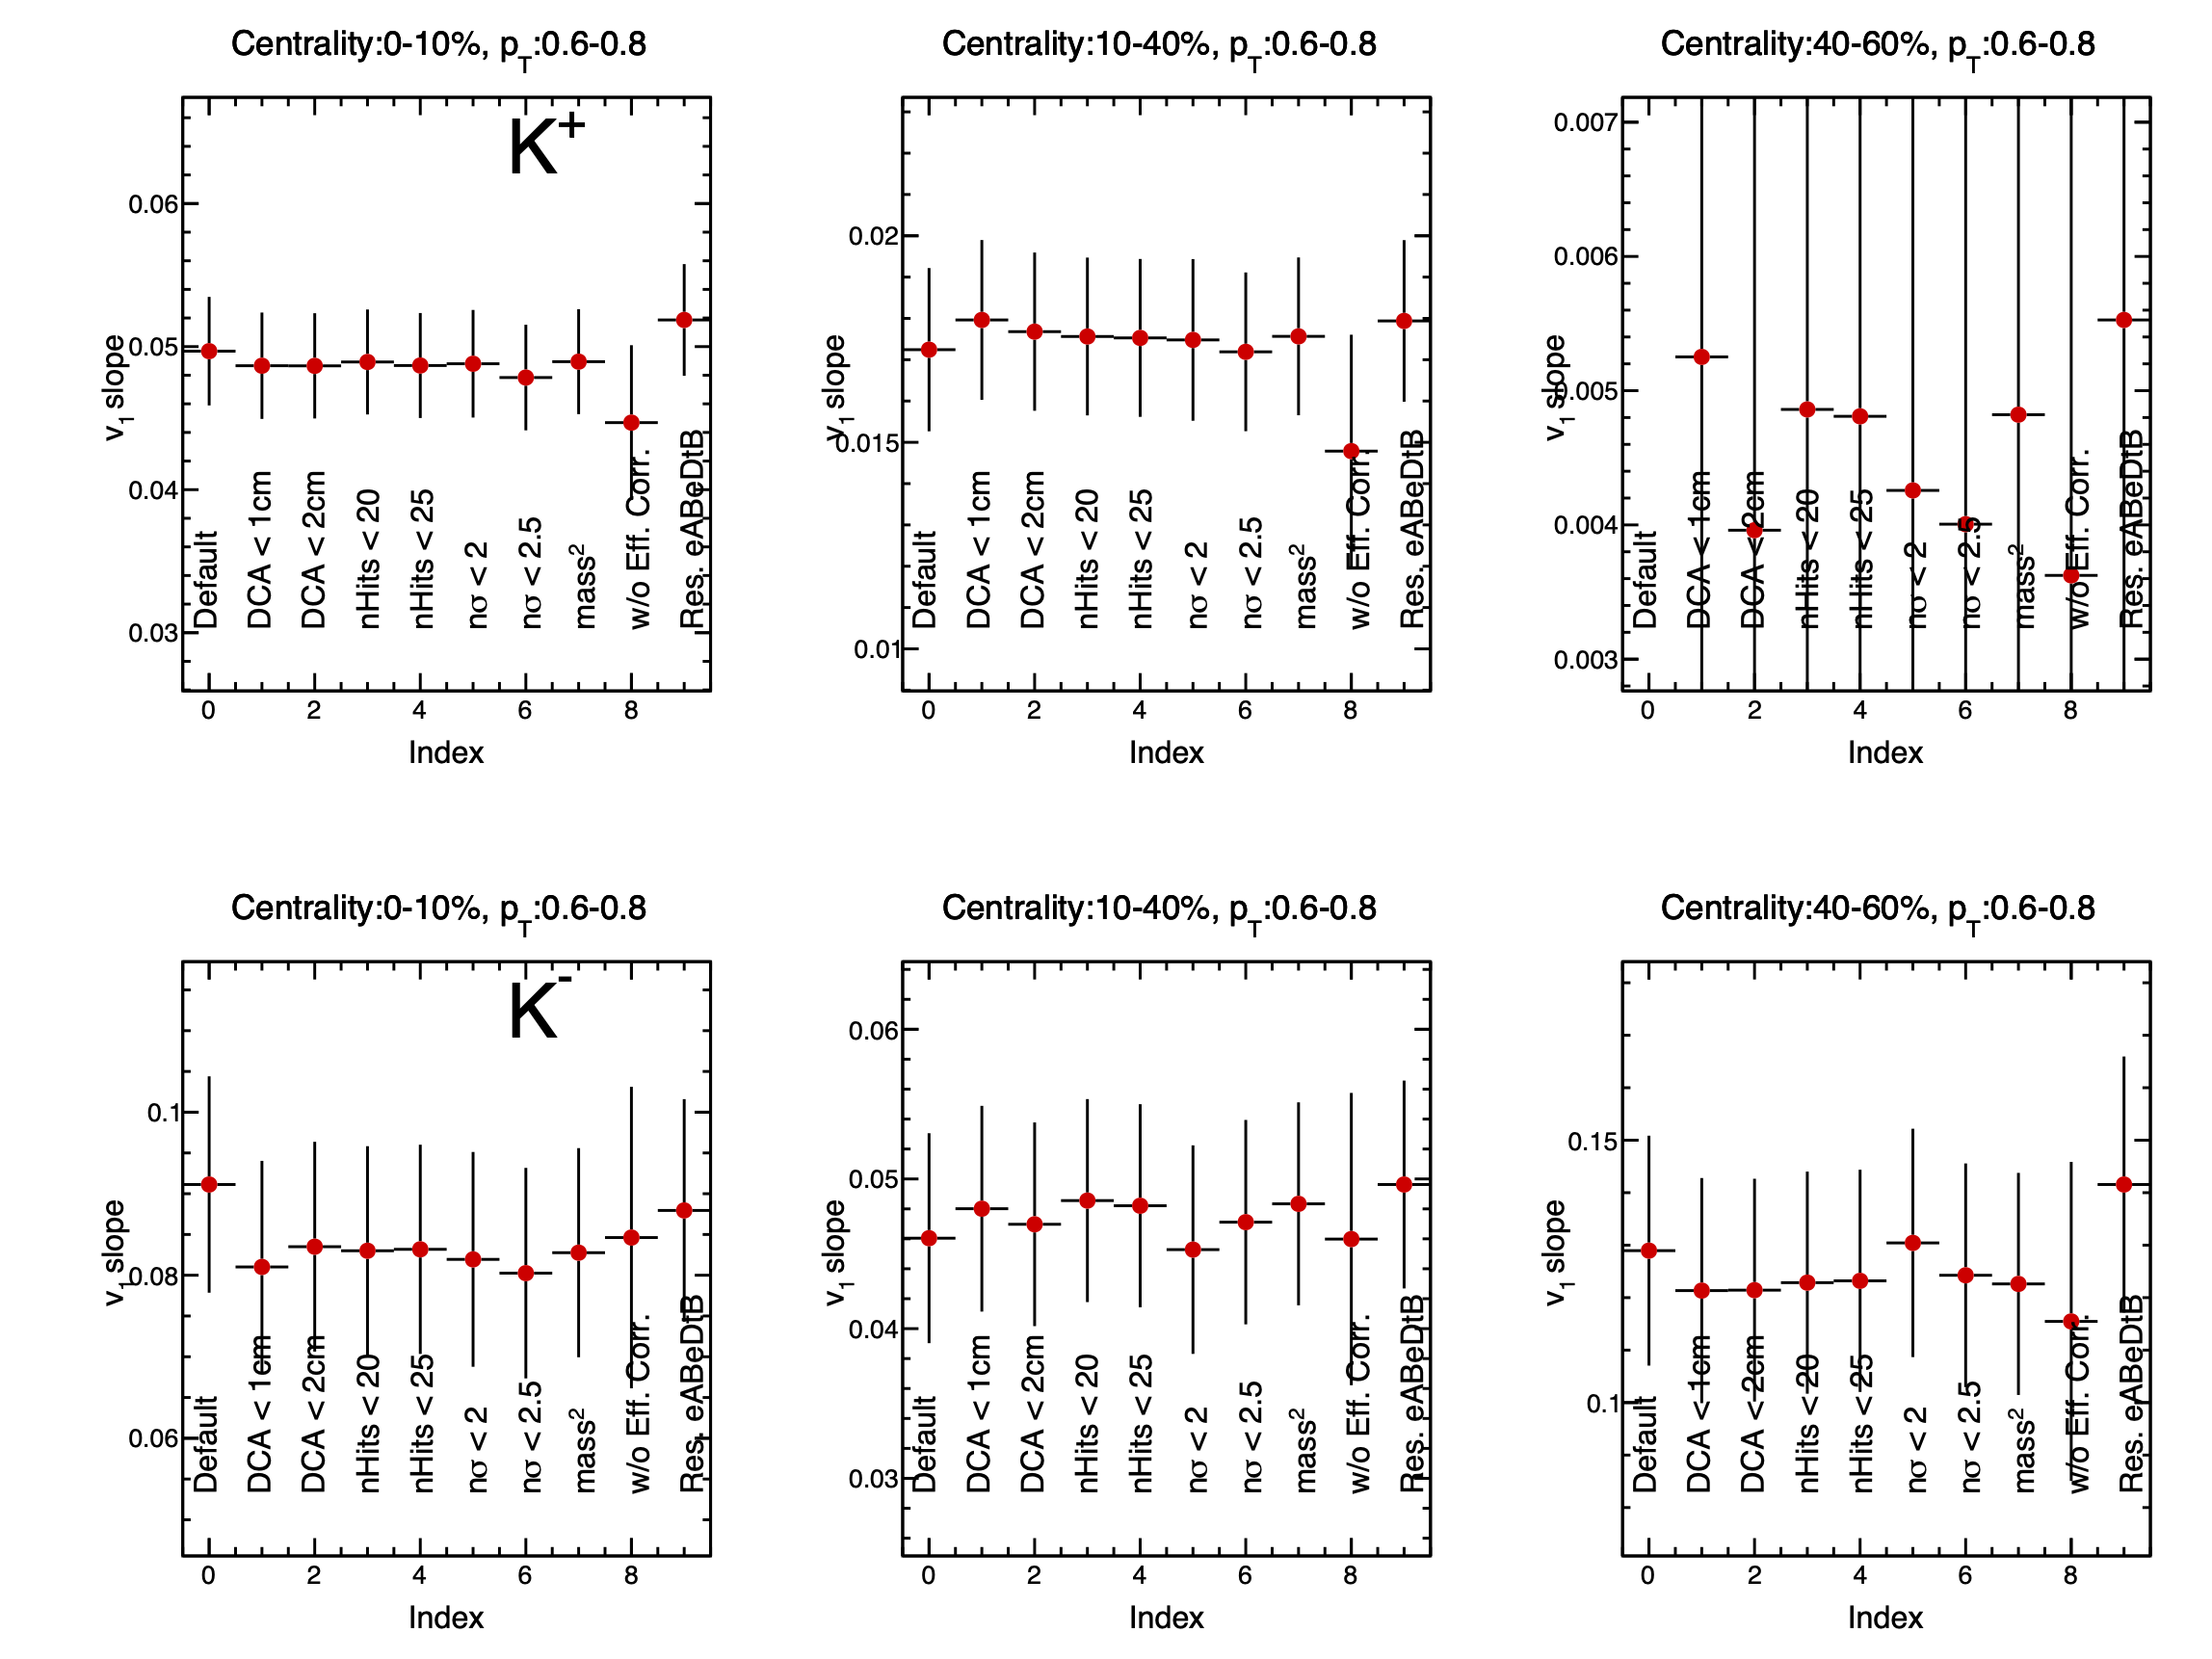
\includegraphics[width=0.85\linewidth]{figures/chapter03/3p5gev_kaon_v1slopeIndex_sysUnc.png}
\caption{$v_1$ slope of kaons as function of systematic sources at $\sqrt{s_{NN}}$ = 3.5 GeV.}
\label{fig:3p5gev_kaon_v1slopeIndex_sysUnc}
\end{figure}

\begin{figure}[hbt!]
\centering
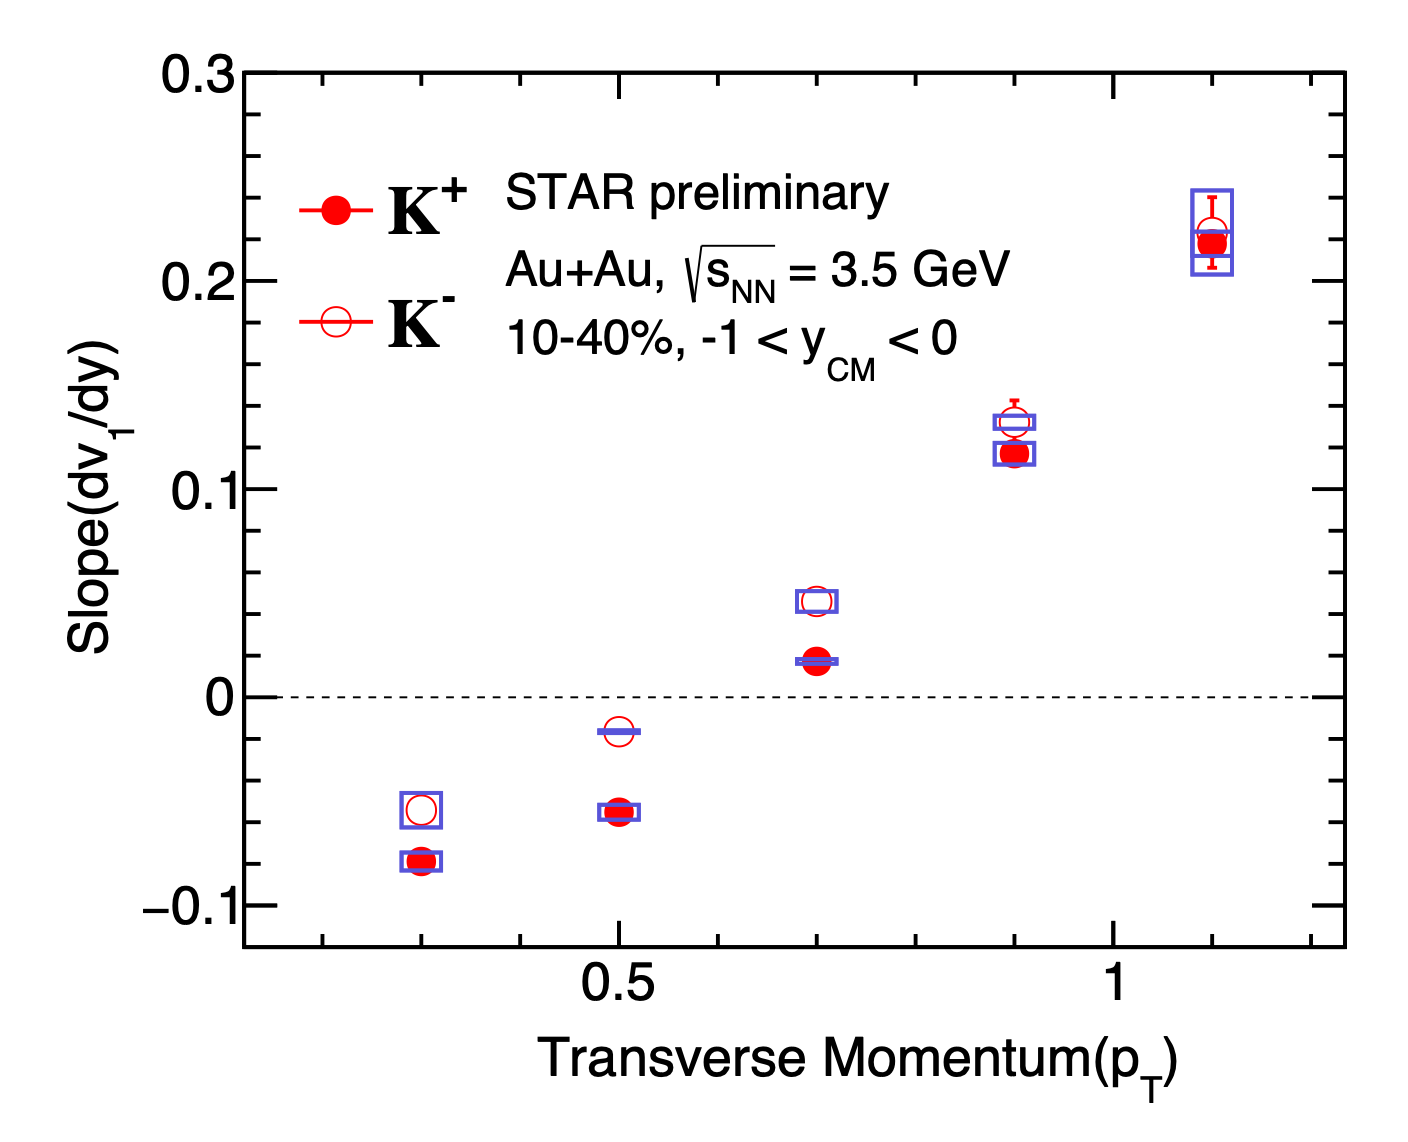
\includegraphics[width=0.55\linewidth]{figures/chapter03/3p5gev_kaon_v1slopePt.png}
\caption{$v_1$ slope of kaons as function of transverse momentum at $\sqrt{s_{NN}}$ = 3.5 GeV.}
\label{fig:3p5gev_kaon_v1slopePt}
\end{figure}


\begin{figure}[hbt!]
\centering
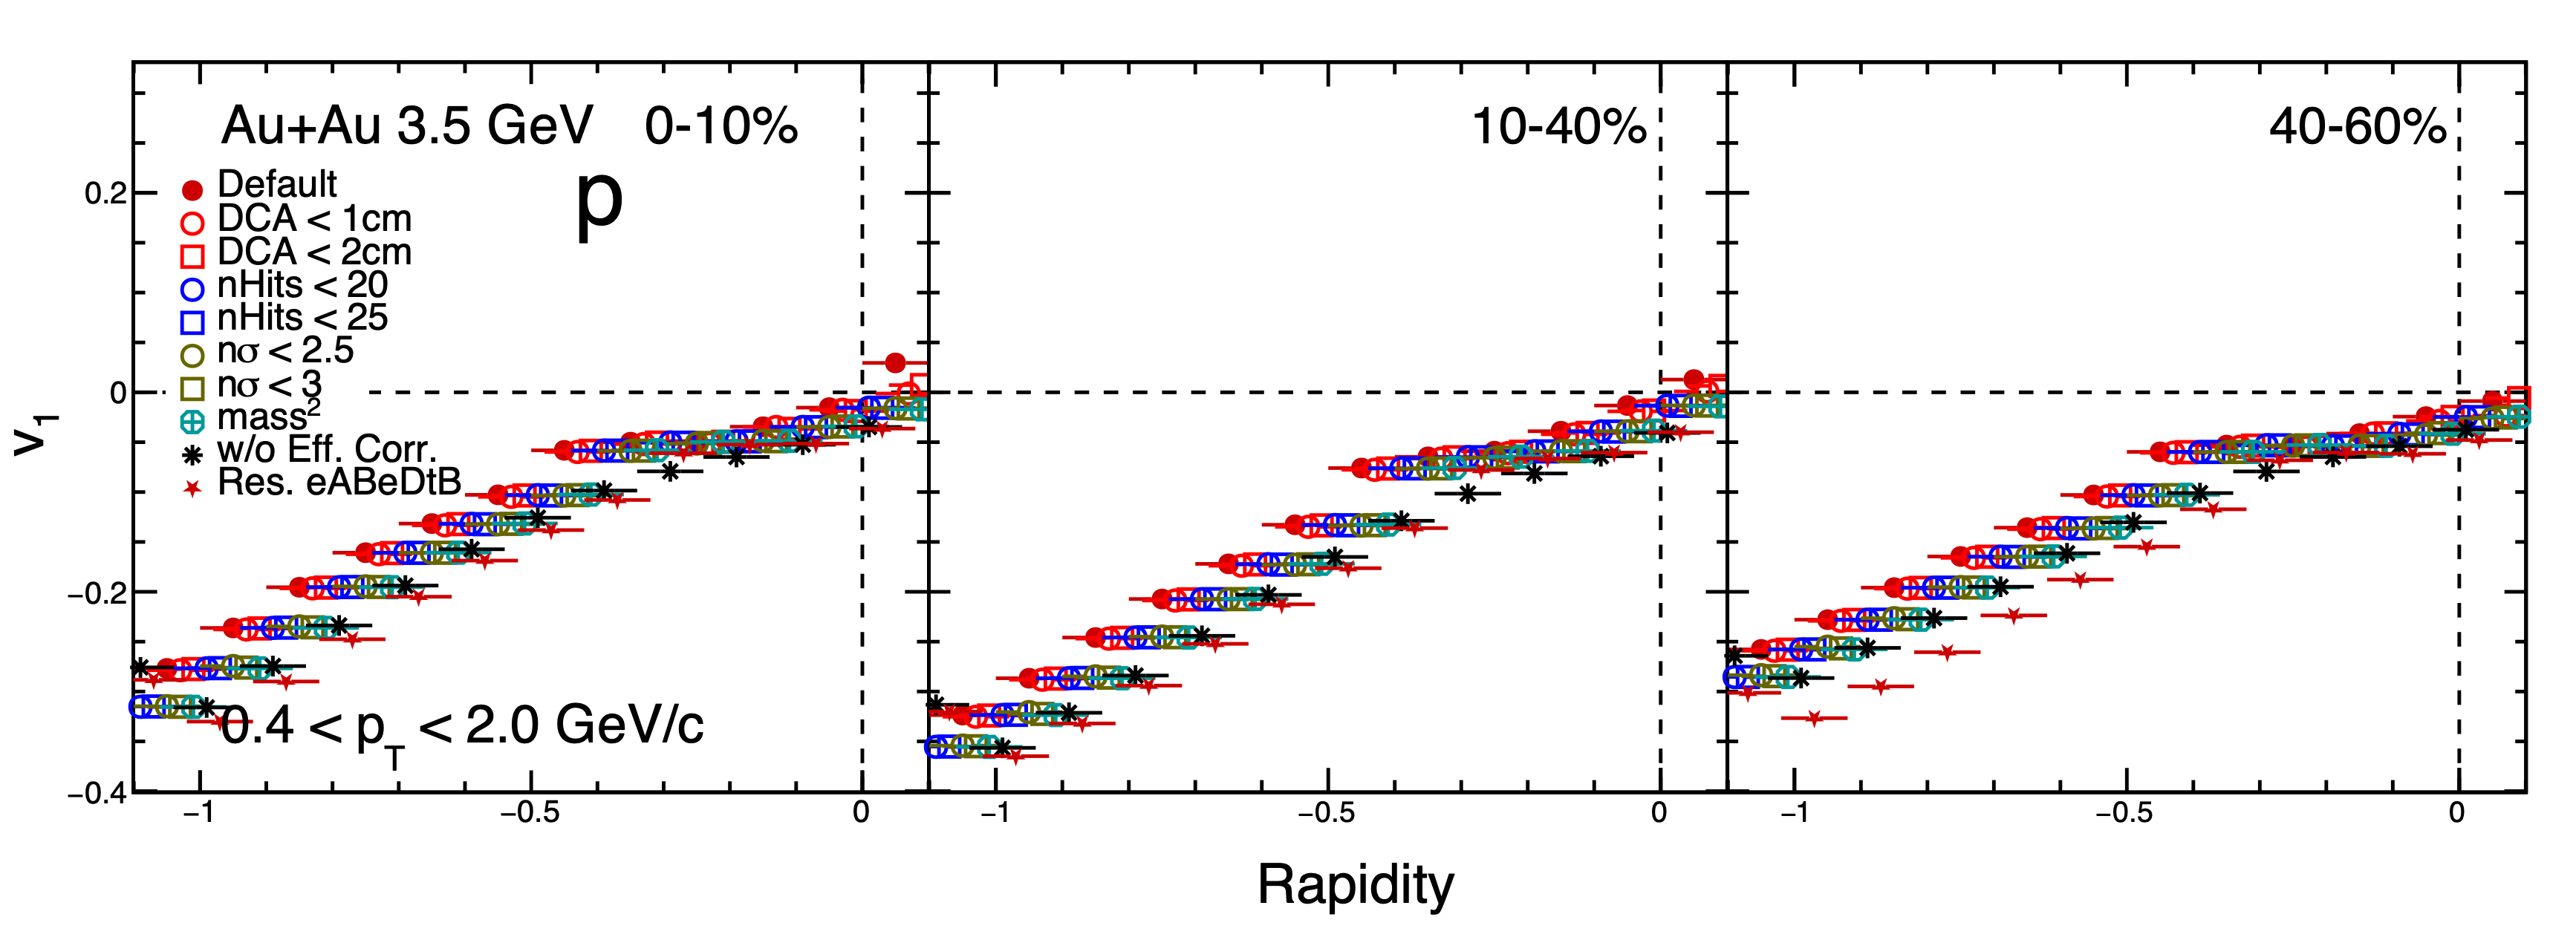
\includegraphics[width=0.95\linewidth]{figures/chapter03/3p5gev_proton_v1y_sysUnc.png}
\caption{$v_1$ of proton as function of rapidity from systematic sources at $\sqrt{s_{NN}}$ = 3.5 GeV.}
\label{fig:3p5gev_proton_v1y_sysUnc}
\end{figure}

\begin{figure}[hbt!]
\centering
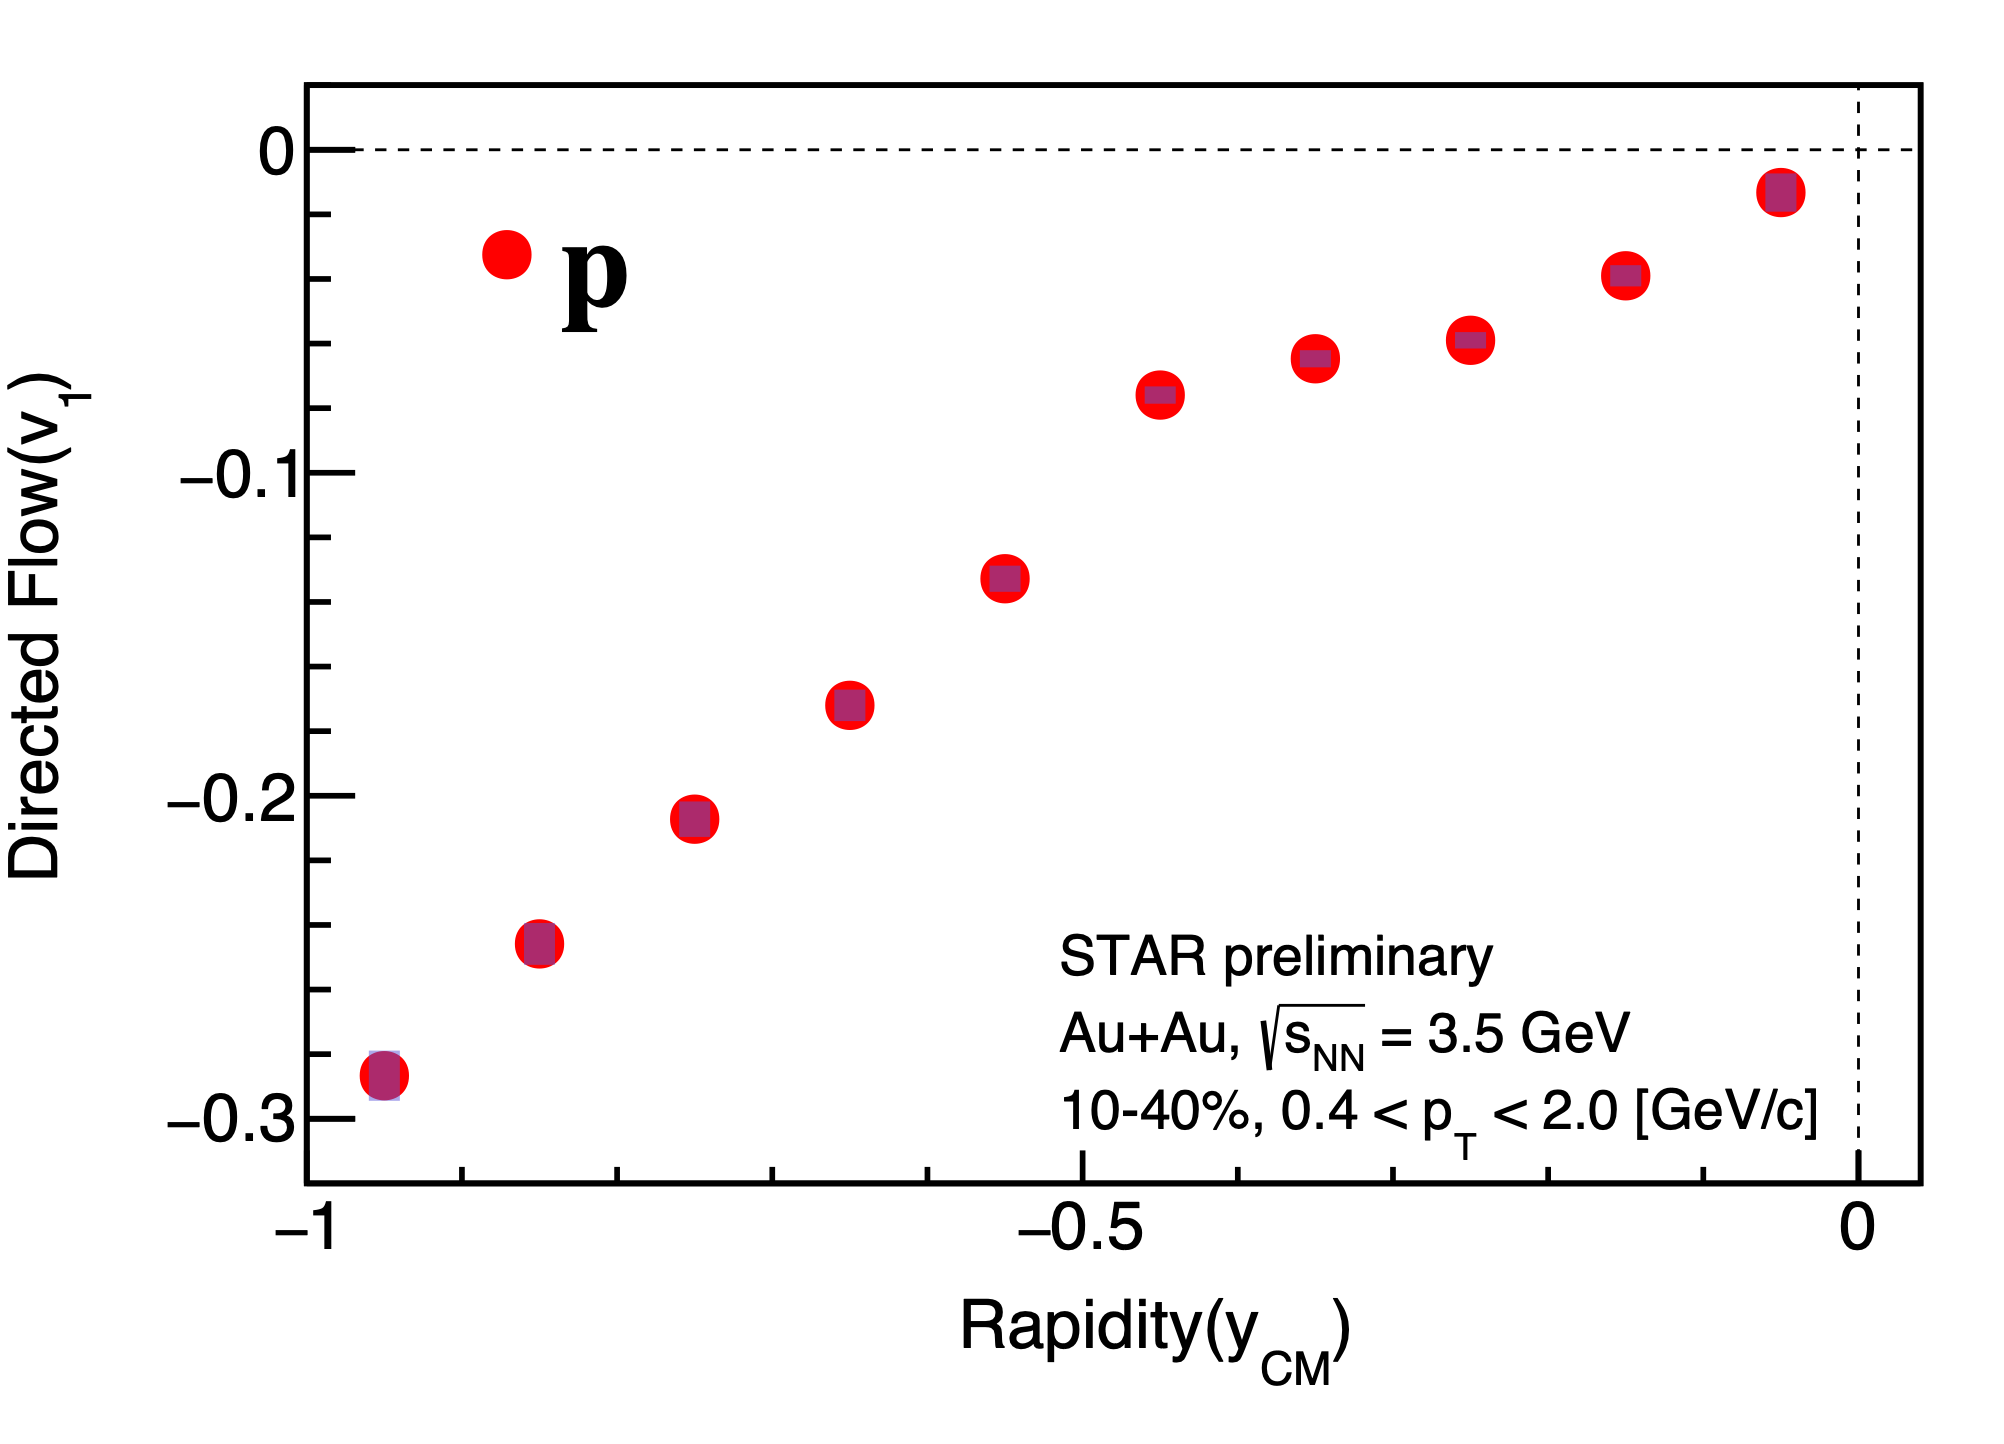
\includegraphics[width=0.65\linewidth]{figures/chapter03/3p5gev_proton_v1y.png}
\caption{$v_1$ of proton as function of rapidity at $\sqrt{s_{NN}}$ = 3.5 GeV.}
\label{fig:3p5gev_proton_v1y}
\end{figure}

\begin{figure}[hbt!]
\centering
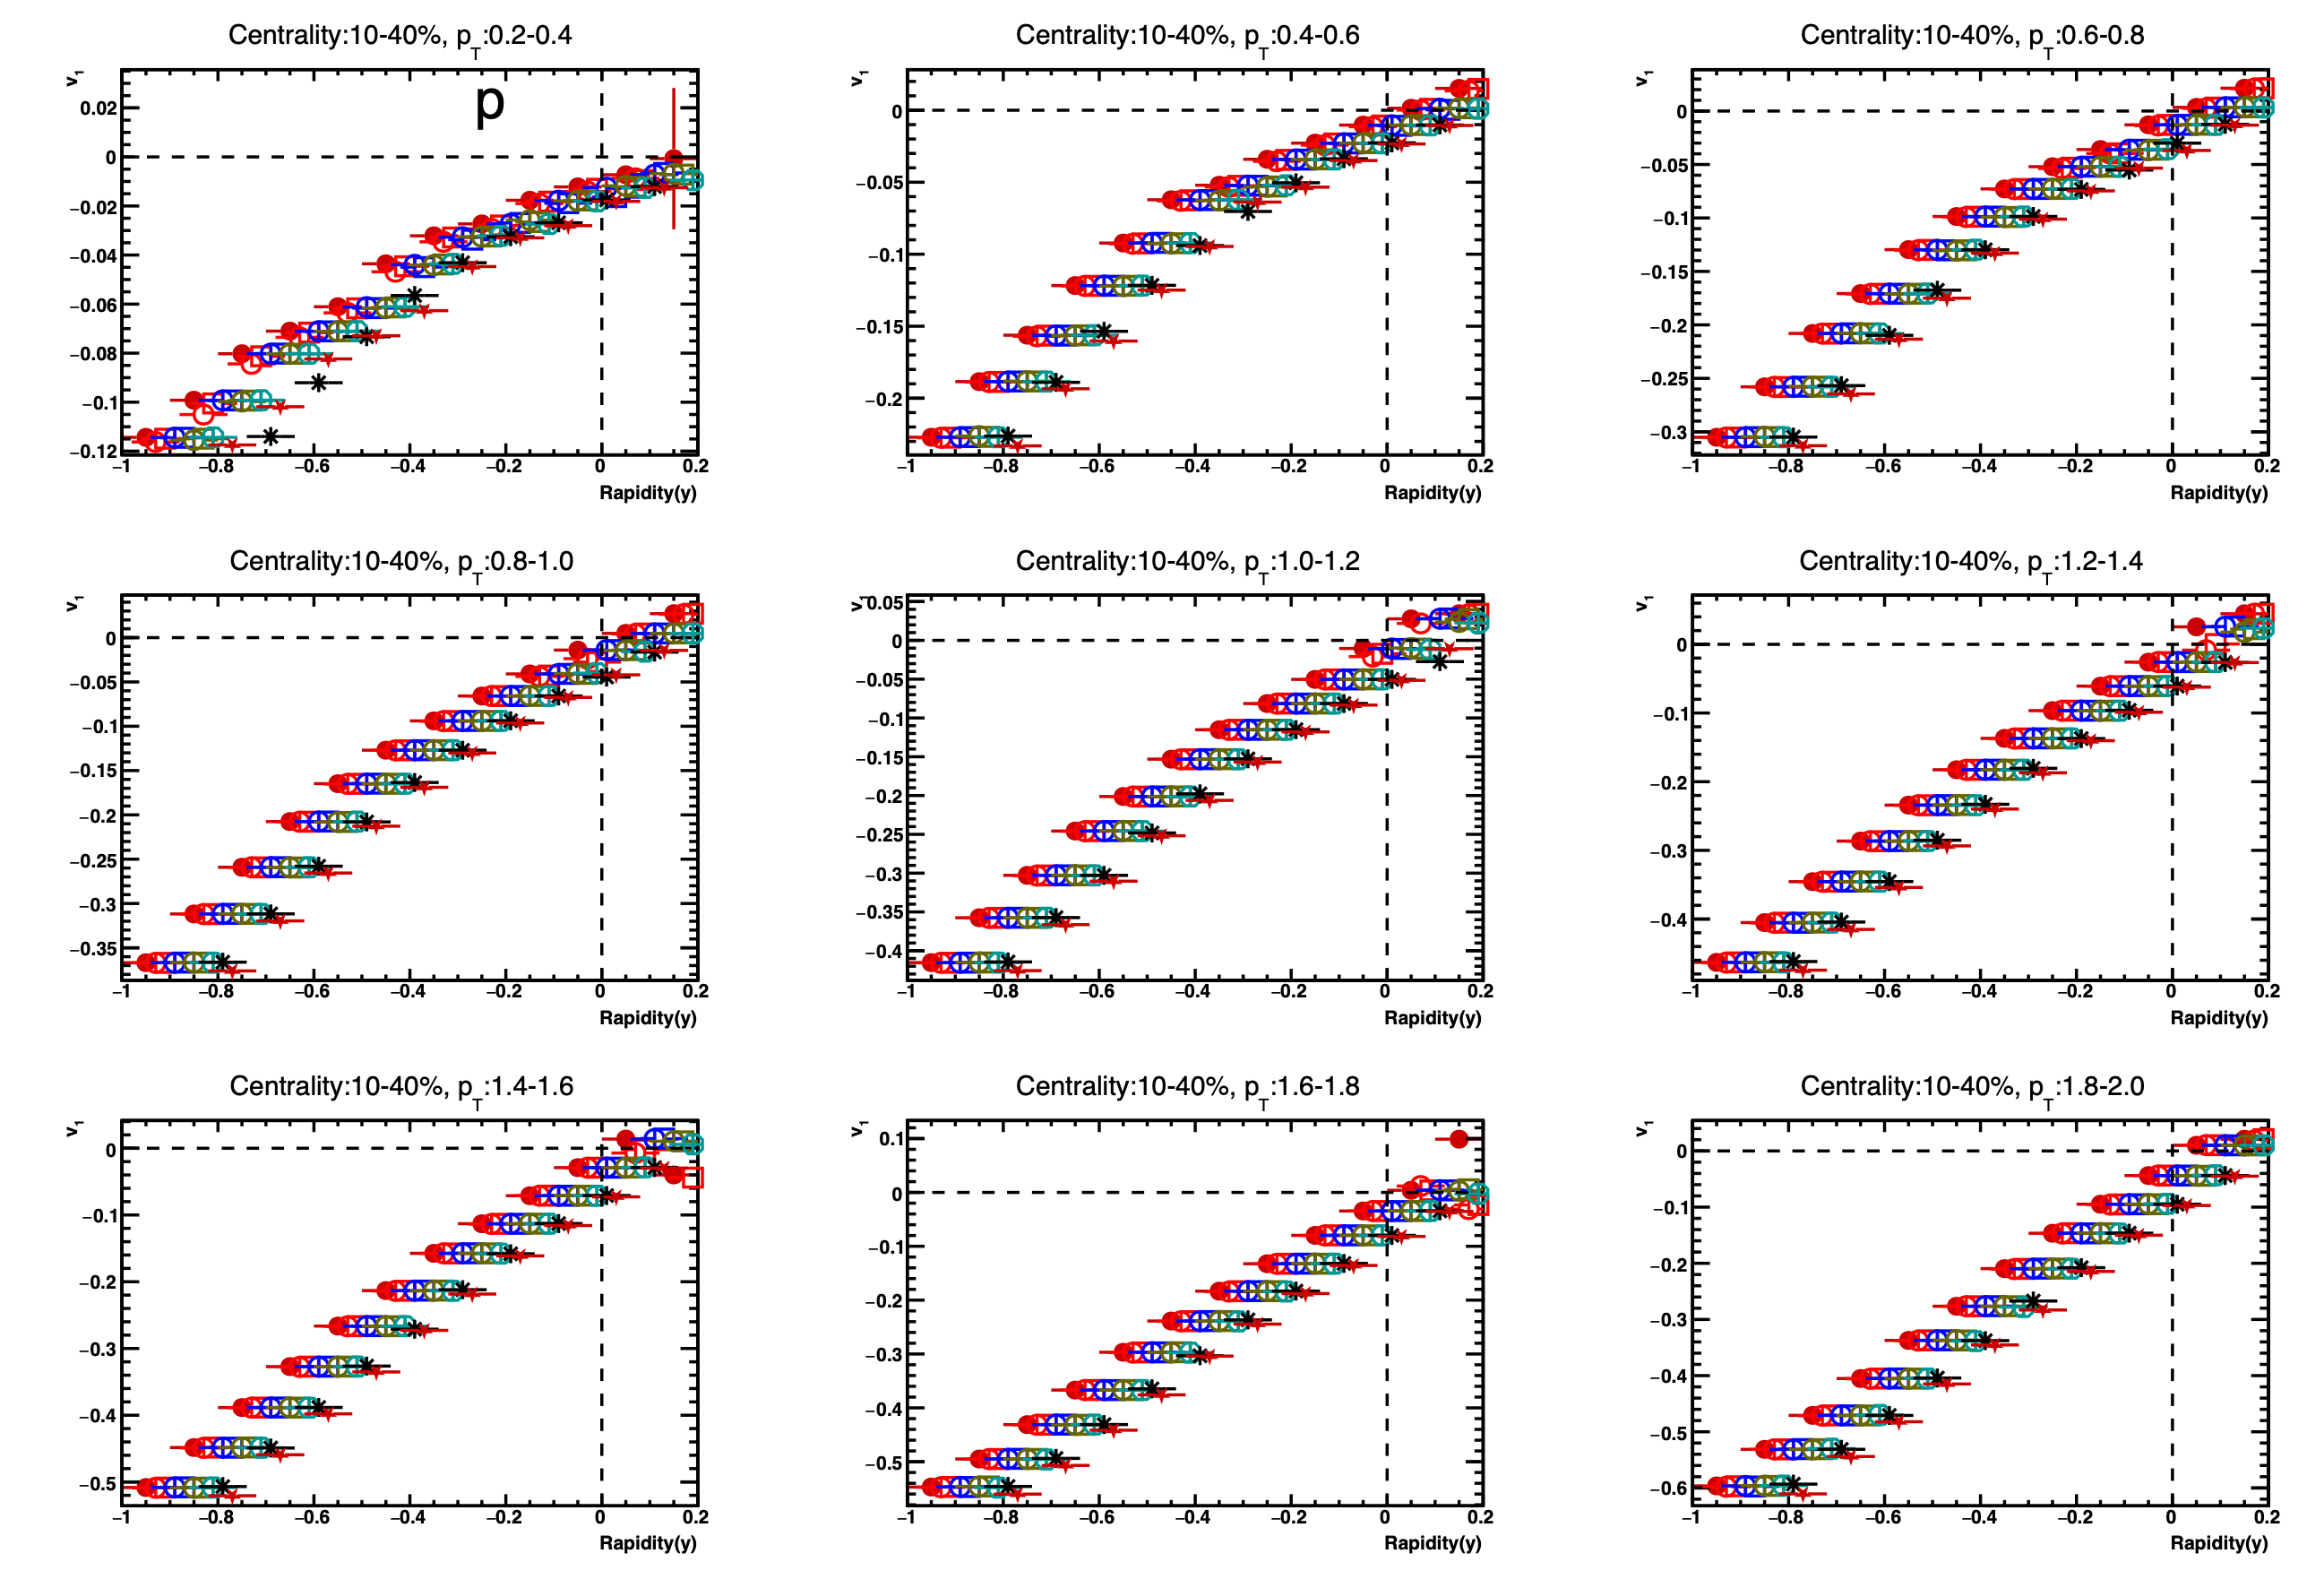
\includegraphics[width=0.95\linewidth]{figures/chapter03/3p5gev_proton_v1yPt_sysUnc.png}
\caption{$v_1$ of p as function of rapidity within $p_T$ windows at $\sqrt{s_{NN}}$ = 3.5 GeV.}
\label{fig:3p5gev_proton_v1yPt_sysUnc}
\end{figure}

\begin{figure}[hbt!]
\centering
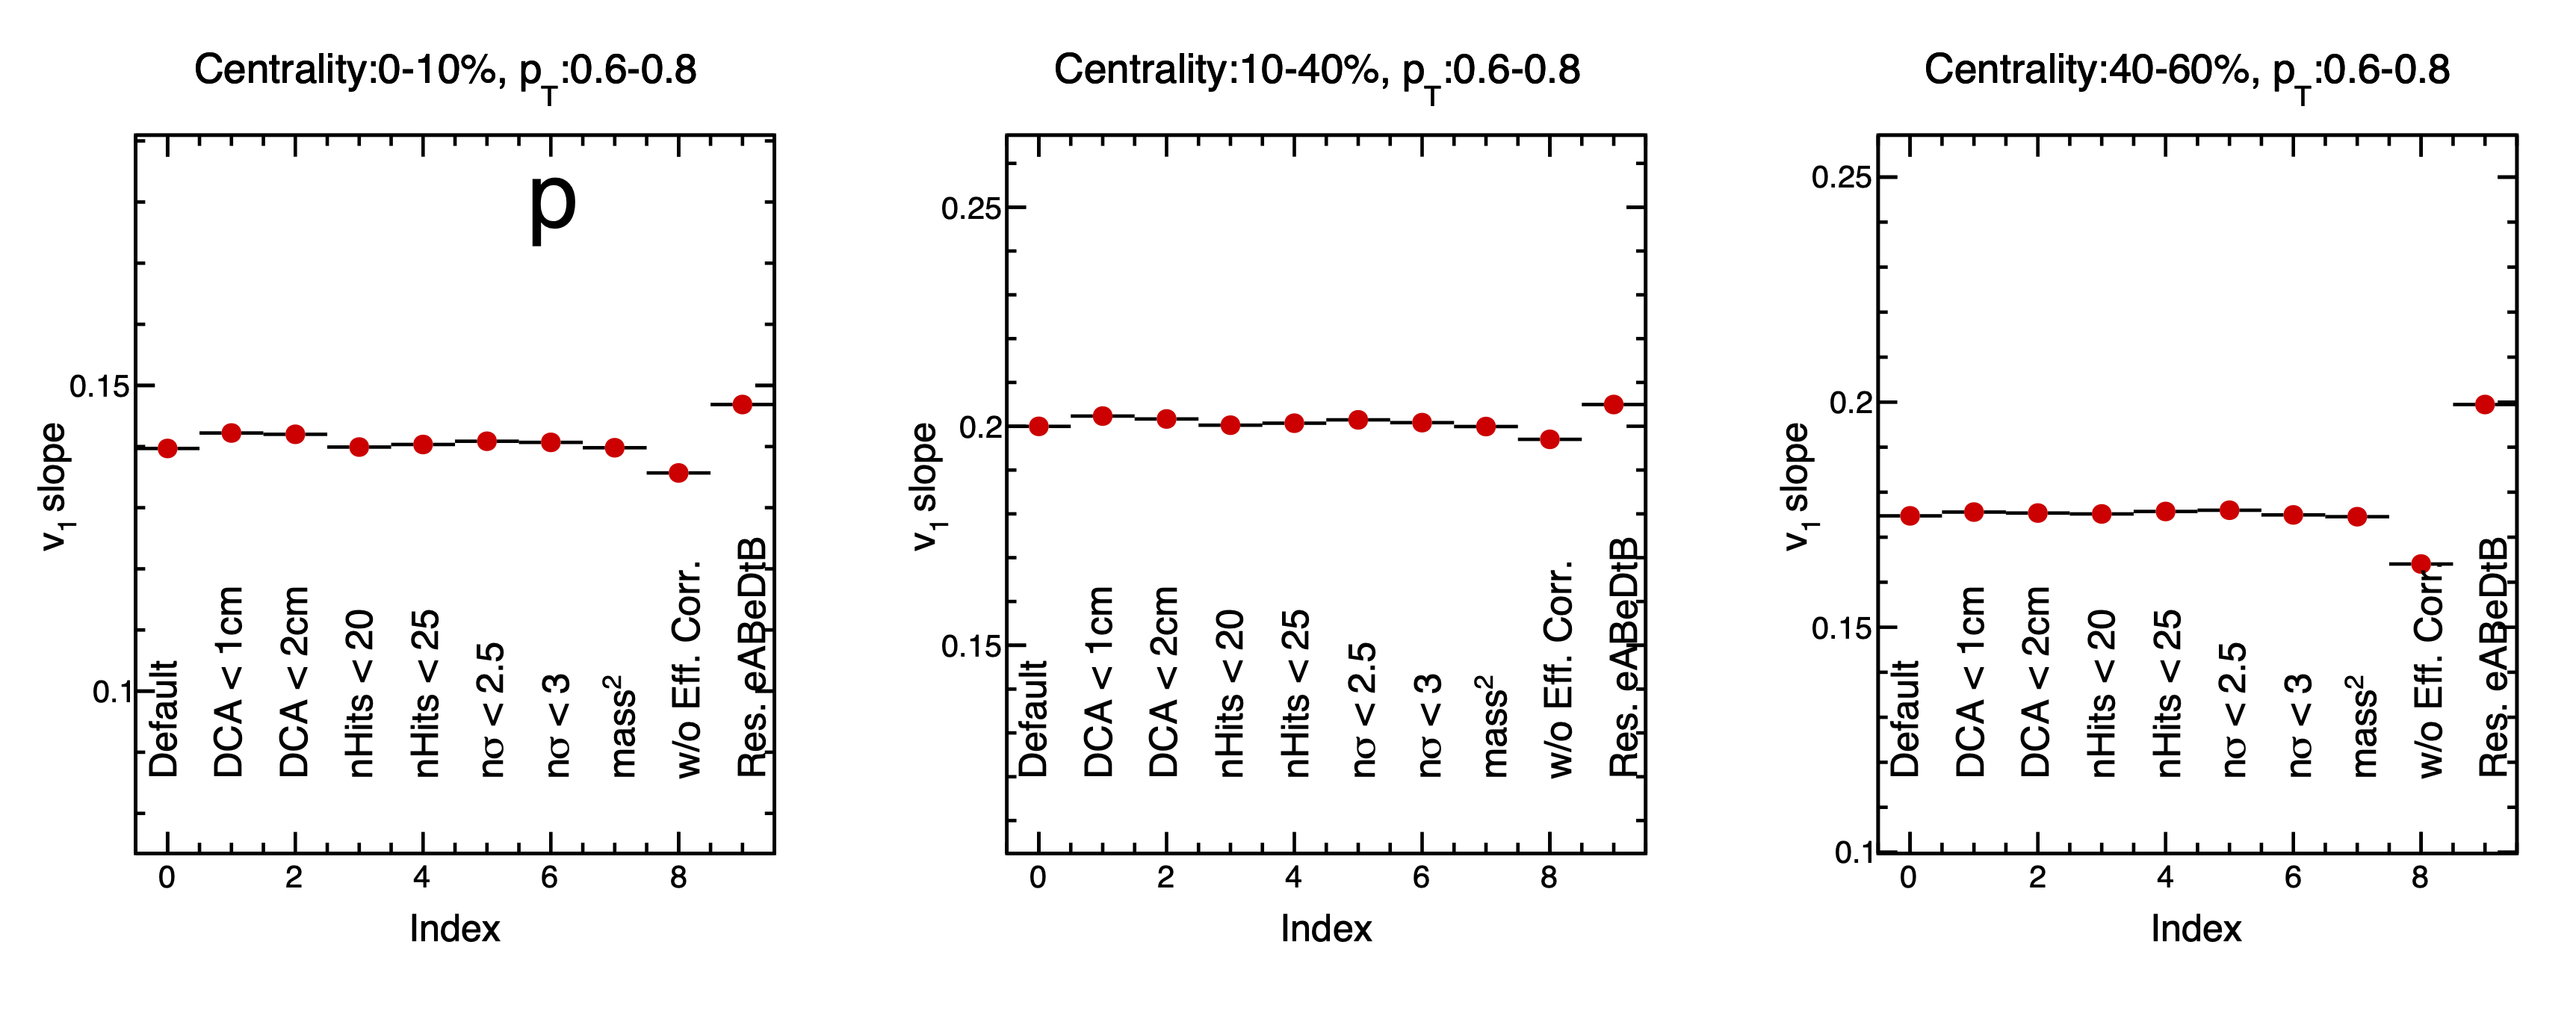
\includegraphics[width=0.85\linewidth]{figures/chapter03/3p5gev_proton_v1slopeIndex_sysUnc.png}
\caption{$v_1$ slope of proton as function of systematic sources at $\sqrt{s_{NN}}$ = 3.5 GeV.}
\label{fig:3p5gev_proton_v1slopeIndex_sysUnc}
\end{figure}

\begin{figure}[hbt!]
\centering
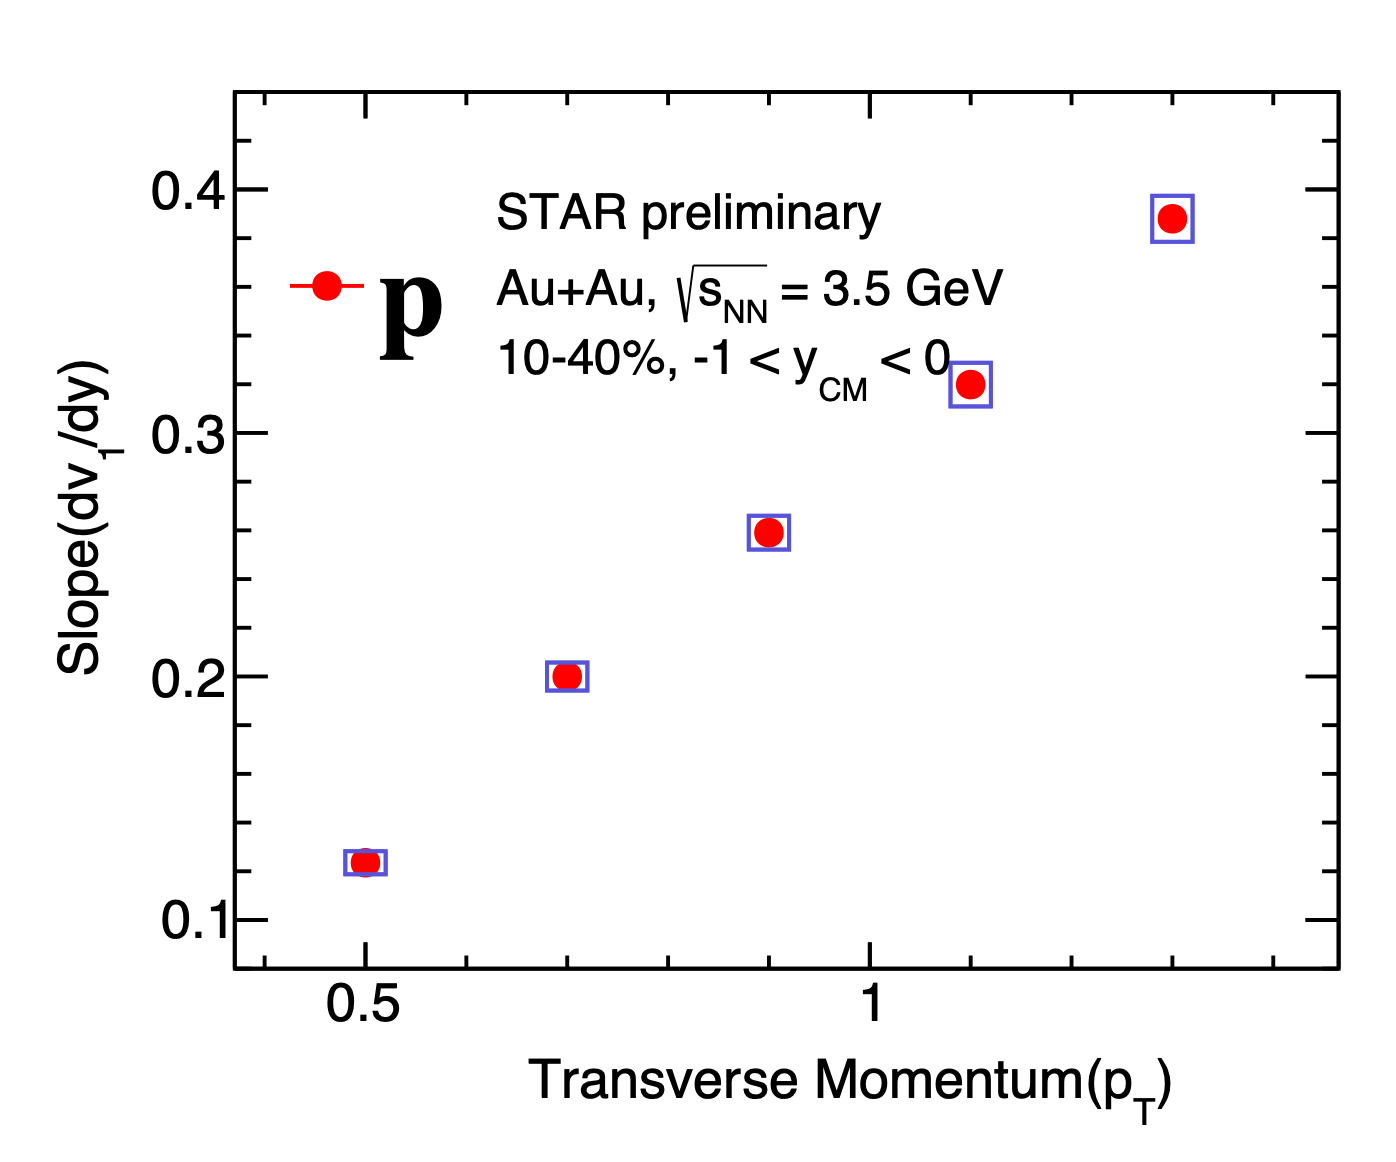
\includegraphics[width=0.55\linewidth]{figures/chapter03/3p5gev_proton_v1slopePt.png}
\caption{$v_1$ slope of proton as function of transverse momentum at $\sqrt{s_{NN}}$ = 3.5 GeV.}
\label{fig:3p5gev_proton_v1slopePt}
\end{figure}